%&preformat-present

\newif\ifpresentation % Условие, проверяющее, что документ --- презентация
\presentationtrue
\documentclass[10pt, xcolor={dvipsnames, table, hyperref}]{beamer}


%%%%%%%%%%%%%%%%%%%%%%%%%%%%%%%%%%%%%%%%%%%%%%%%%%%%%%%%%%%%%%%%%%%%%%%%%%%%%%%%
%%%% Файл упрощённых настроек шаблона, общих для диссертации и автореферата %%%%
%%%%%%%%%%%%%%%%%%%%%%%%%%%%%%%%%%%%%%%%%%%%%%%%%%%%%%%%%%%%%%%%%%%%%%%%%%%%%%%%

%%% Режим черновика %%%
\makeatletter
\@ifundefined{c@draft}{
  \newcounter{draft}
  \setcounter{draft}{1}  % 0 --- чистовик (максимальное соблюдение ГОСТ)
                         % 1 --- черновик (отклонения от ГОСТ, но быстрая
                         %       сборка итоговых PDF)
}{}
\makeatother

%%% Использование в pdflatex шрифтов не по-умолчанию %%%
\makeatletter
\@ifundefined{c@usealtfont}{
  \newcounter{usealtfont}
  \setcounter{usealtfont}{1}    % 0 --- шрифты на базе Computer Modern
                                % 1 --- использовать пакет pscyr, при его
                                %       наличии
                                % 2 --- использовать пакет XCharter, при наличии
                                %       подходящей версии
}{}
\makeatother

%%% Использование в xelatex и lualatex семейств шрифтов %%%
\makeatletter
\@ifundefined{c@fontfamily}{
  \newcounter{fontfamily}
  \setcounter{fontfamily}{1}  % 0 --- CMU семейство. Используется как fallback;
                              % 1 --- Шрифты от MS (Times New Roman и компания)
                              % 2 --- Семейство Liberation
}{}
\makeatother

%%% Библиография %%%
\makeatletter
\@ifundefined{c@bibliosel}{
  \newcounter{bibliosel}
  \setcounter{bibliosel}{1}   % 0 --- встроенная реализация с загрузкой файла
                              %       через движок bibtex8;
                              % 1 --- реализация пакетом biblatex через движок
                              %       biber
}{}
\makeatother

%%% Предкомпиляция tikz рисунков для ускорения работы %%%
\makeatletter
\@ifundefined{c@imgprecompile}{
  \newcounter{imgprecompile}
  \setcounter{imgprecompile}{0}   % 0 --- без предкомпиляции;
                                  % 1 --- пользоваться предварительно
                                  %       скомпилированными pdf вместо генерации
                                  %       заново из tikz
}{}
\makeatother
               % Общие настройки шаблона
%%% Проверка используемого TeX-движка %%%
\newif\ifxetexorluatex   % определяем новый условный оператор (http://tex.stackexchange.com/a/47579)
\ifxetex
    \xetexorluatextrue
\else
    \ifluatex
        \xetexorluatextrue
    \else
        \xetexorluatexfalse
    \fi
\fi

\newif\ifsynopsis           % Условие, проверяющее, что документ --- автореферат

\usepackage{etoolbox}[2015/08/02]               % Для продвинутой проверки разных условий
\providebool{presentation}

%%% Поля и разметка страницы %%%
\usepackage{pdflscape}                              % Для включения альбомных страниц
\usepackage{geometry}                               % Для последующего задания полей

%%% Математические пакеты %%%
\usepackage{amsthm,amsmath,amscd}   % Математические дополнения от AMS
\usepackage{amsfonts,amssymb}       % Математические дополнения от AMS
\usepackage{mathtools}              % Добавляет окружение multlined
\usepackage{xfrac}                  % Красивые дроби
\usepackage[
    locale = DE,
    list-separator       = {;\,},
    list-final-separator = {;\,},
    list-pair-separator  = {;\,},
    range-phrase={\text{\ensuremath{-}}},
    % quotient-mode        = fraction, % красивые дроби могут не соответствовать ГОСТ
    fraction-function    = \sfrac,
    separate-uncertainty,
    ]{siunitx}                      % Размерности SI
\sisetup{inter-unit-product = \ensuremath{{}\cdot{}}}

% Кириллица в нумерации subequations
% Для правильной работы требуется выполнение сразу после загрузки пакетов
\patchcmd{\subequations}{\def\theequation{\theparentequation\alph{equation}}}
{\def\theequation{\theparentequation\asbuk{equation}}}
{\typeout{subequations patched}}{\typeout{subequations not patched}}

%%%% Установки для размера шрифта 14 pt %%%%
%% Формирование переменных и констант для сравнения (один раз для всех подключаемых файлов)%%
%% должно располагаться до вызова пакета fontspec или polyglossia, потому что они сбивают его работу
\newlength{\curtextsize}
\newlength{\bigtextsize}
\setlength{\bigtextsize}{13.9pt}

\makeatletter
%\show\f@size                                       % неплохо для отслеживания, но вызывает стопорение процесса, если документ компилируется без команды  -interaction=nonstopmode
\setlength{\curtextsize}{\f@size pt}
\makeatother

%%% Кодировки и шрифты %%%
\ifxetexorluatex
    \PassOptionsToPackage{no-math}{fontspec}        % https://tex.stackexchange.com/a/26295/104425
    \usepackage{polyglossia}[2014/05/21]            % Поддержка многоязычности (fontspec подгружается автоматически)
\else
   %%% Решение проблемы копирования текста в буфер кракозябрами
    \ifnumequal{\value{usealtfont}}{0}{}{
        \input glyphtounicode.tex
        \input glyphtounicode-cmr.tex %from pdfx package
        \pdfgentounicode=1
    }
    \usepackage{cmap}                               % Улучшенный поиск русских слов в полученном pdf-файле
    \ifnumequal{\value{usealtfont}}{2}{}{
        \defaulthyphenchar=127                      % Если стоит до fontenc, то переносы не впишутся в выделяемый текст при копировании его в буфер обмена
    }
    \usepackage{textcomp}
    \usepackage[T1,T2A]{fontenc}                    % Поддержка русских букв
    \ifnumequal{\value{usealtfont}}{1}{% Используется pscyr, при наличии
        \IfFileExists{pscyr.sty}{\usepackage{pscyr}}{}  % Подключение pscyr
    }{}
    \usepackage[utf8]{inputenc}[2014/04/30]         % Кодировка utf8
    \usepackage[english, russian]{babel}[2014/03/24]% Языки: русский, английский
    \ifnumequal{\value{usealtfont}}{2}{
        % http://dxdy.ru/post1238763.html#p1238763
        \usepackage[scaled=0.960]{XCharter}[2017/12/19] % Подключение русифицированных шрифтов XCharter
        \usepackage[charter, vvarbb, scaled=1.048]{newtxmath}[2017/12/14]
        \ifpresentation
        \else
            \setDisplayskipStretch{-0.078}
        \fi
    }{}
\fi

%%% Оформление абзацев %%%
\usepackage{indentfirst}                            % Красная строка

%%% Цвета %%%
\ifpresentation
\else
    \usepackage[dvipsnames, table, hyperref]{xcolor} % Совместимо с tikz
\fi

%%% Таблицы %%%
\usepackage{longtable,ltcaption} % Длинные таблицы
\usepackage{multirow,makecell}   % Улучшенное форматирование таблиц
\usepackage{tabu, tabulary}      % таблицы с автоматически подбирающейся
                                 % шириной столбцов (tabu обязательно
                                 % до hyperref вызывать)
\usepackage{threeparttable}      % автоматический подгон ширины подписи таблицы

%%% Общее форматирование
\usepackage{soulutf8}                               % Поддержка переносоустойчивых подчёркиваний и зачёркиваний
\usepackage{icomma}                                 % Запятая в десятичных дробях

%%% Оптимизация расстановки переносов и длины последней строки абзаца
\IfFileExists{impnattypo.sty}{% проверка установленности пакета impnattypo
    \ifluatex
        \ifnumequal{\value{draft}}{1}{% Черновик
            \usepackage[hyphenation, lastparline, nosingleletter, homeoarchy,
            rivers, draft]{impnattypo}
        }{% Чистовик
            \usepackage[hyphenation, lastparline, nosingleletter]{impnattypo}
        }
    \else
        \usepackage[hyphenation, lastparline]{impnattypo}
    \fi
}{}

%% Векторная графика

\usepackage{tikz}                   % Продвинутый пакет векторной графики
\usetikzlibrary{chains}             % Для примера tikz рисунка
\usetikzlibrary{shapes.geometric}   % Для примера tikz рисунка
\usetikzlibrary{shapes.symbols}     % Для примера tikz рисунка
\usetikzlibrary{arrows}             % Для примера tikz рисунка

%%% Гиперссылки %%%
\usepackage{hyperref}[2012/11/06]

%%% Изображения %%%
\usepackage{graphicx}[2014/04/25]                   % Подключаем пакет работы с графикой
\usepackage{media9}

%%% Счётчики %%%
\usepackage[figure,table]{totalcount}               % Счётчик рисунков и таблиц
\usepackage{totcount}                               % Пакет создания счётчиков на основе последнего номера подсчитываемого элемента (может требовать дважды компилировать документ)
\usepackage{totpages}                               % Счётчик страниц, совместимый с hyperref (ссылается на номер последней страницы). Желательно ставить последним пакетом в преамбуле

%%% Продвинутое управление групповыми ссылками (пока только формулами) %%%
\ifpresentation
\else
    \usepackage[russian]{cleveref} % cleveref имеет сложности со считыванием
    % языка из babel. Такое решение русификации вывода выбрано вместо
    % определения в documentclass из опасности что-то лишнее передать во все
    % остальные пакеты, включая библиографию.
    \creflabelformat{equation}{#2#1#3} % Формат по умолчанию ставил круглые
    % скобки вокруг каждого номера ссылки, теперь просто номера ссылок без
    % какого-либо дополнительного оформления
    \crefrangelabelformat{equation}{#3#1#4\cyrdash#5#2#6} % Интервалы в русском
    % языке принято делать через тире, если иное не оговорено

    % решение проблемы с "и" в \labelcref
    % https://tex.stackexchange.com/a/455124/104425
    \ifxetexorluatex
        \DeclareTextSymbol{\cyri}\UnicodeEncodingName{"0438} % и
    \fi

    % Добавление возможности использования пробелов в \labelcref
    % https://tex.stackexchange.com/a/340502/104425
    \usepackage{kvsetkeys}
    \makeatletter
    \let\org@@cref\@cref
    \renewcommand*{\@cref}[2]{%
        \edef\process@me{%
            \noexpand\org@@cref{#1}{\zap@space#2 \@empty}%
        }\process@me
    }
    \makeatother

    \newcommand{\eqrefs}[1]{(\labelcref{#1})}
    \newcommand{\refs}[1]{\labelcref{#1}}
\fi

\ifnumequal{\value{draft}}{1}{% Черновик
    \usepackage[firstpage]{draftwatermark}
    \SetWatermarkText{DRAFT}
    \SetWatermarkFontSize{14pt}
    \SetWatermarkScale{15}
    \SetWatermarkAngle{45}
}{}

%%% Исправление положения якорей подписей (под)рисунков %%%
% Без hypcap и патча, при клике по ссылке на подрисунок, просмотрщик pdf прыгает "к подписи" а не "к рисунку".
% Подробнее: https://github.com/AndreyAkinshin/Russian-Phd-LaTeX-Dissertation-Template/issues/238
% (!) Даже с патчем, если мешать в одной фиге разные типы подфиг (subbottom и subcaption) - ссылки всё равно будут работать неправильно  (см. https://www.overleaf.com/read/czmbmmtnqrrg ).
\ifpresentation
\else
    \usepackage[all]{hypcap}

    \makeatletter
    \ltx@ifclasslater{memoir}{2018/12/13}{
        % Предполагается, что в следующей версии класс будет исправлен
        \typeout{Assuming this version of memoir is free from the jumping-to-caption bug.}
    }{
        \usepackage{xpatch}

        \newcommand\mem@step@subcounter{\refstepcounter{sub\@captype}\@contkeep}

        \xpatchcmd{\@memsubbody}%
        {\refstepcounter{sub\@captype}\@contkeep}% search pattern
        {}% replacement
        {\typeout{@memsubbody is patched}}%
        {\typeout{@memsubbody is NOT patched}}%

        \xpatchcmd{\@memcontsubbody}%
        {\refstepcounter{sub\@captype}\@contkeep}% pattern
        {}% replacement
        {\typeout{@memcontsubbody is patched}}%
        {\typeout{@memcontsubbody is NOT patched}}%

        \xpatchcmd{\@memsubfloat}%
        {\vbox\bgroup}% search pattern
        {\vbox\bgroup\mem@step@subcounter}% replacement
        {\typeout{@memsubfloat patch is ok}}%
        {\typeout{@memsubfloat patch is NOT ok}}%

        \xpatchcmd{\subcaption}%
        {\refstepcounter{sub\@captype}}% search pattern
        {\H@refstepcounter{sub\@captype}}% replacement
        {\typeout{subcaption second patch is ok}}%
        {\typeout{subcaption second patch is NOT ok}}%
    }
    \makeatother
\fi

%%% Цитата, не приводимая в автореферате:
% возможно, актуальна только для biblatex
%\newcommand{\citeinsynopsis}[1]{\ifsynopsis\else ~\cite{#1} \fi}

% если текущий процесс запущен библиотекой tikz-external, то прекомпиляция должна быть включена
\ifdefined\tikzexternalrealjob
    \setcounter{imgprecompile}{1}
\fi

\ifnumequal{\value{imgprecompile}}{1}{% Только если у нас включена предкомпиляция
    \usetikzlibrary{external}   % подключение возможности предкомпиляции
    \tikzexternalize[prefix=images/cache/] % activate! % здесь можно указать отдельную папку для скомпилированных файлов
    \ifxetex
        \tikzset{external/up to date check={diff}}
    \fi
}{}
            % Пакеты общие для диссертации и автореферата
%%% Основные сведения %%%
\newcommand{\thesisAuthorLastName}{Клековкин}
\newcommand{\thesisAuthorOtherNames}{Антон Владимирович}
\newcommand{\thesisAuthorInitials}{{А.\,В.}}
\newcommand{\thesisAuthor}             % Диссертация, ФИО автора
{%
    \texorpdfstring{% \texorpdfstring takes two arguments and uses the first for (La)TeX and the second for pdf
        \thesisAuthorLastName~\thesisAuthorOtherNames% так будет отображаться на титульном листе или в тексте, где будет использоваться переменная
    }{%
        \thesisAuthorLastName, \thesisAuthorOtherNames% эта запись для свойств pdf-файла. В таком виде, если pdf будет обработан программами для сбора библиографических сведений, будет правильно представлена фамилия.
    }
}
\newcommand{\thesisAuthorShort}        % Диссертация, ФИО автора инициалами
{\thesisAuthorInitials~\thesisAuthorLastName}
%\newcommand{\thesisUdk}                % Диссертация, УДК
%{\todo{xxx.xxx}}
\newcommand{\thesisTitle}              % Диссертация, название
{Исследование динамики безвинтовых роботов в жидкости с неизменяемой формой оболочки и управляемых внутренними роторами}
\newcommand{\thesisSpecialtyNumber}    % Диссертация, специальность, номер
{{05.02.05}}
\newcommand{\thesisSpecialtyTitle}     % Диссертация, специальность, название (название взято с сайта ВАК для примера)
{Роботы, мехатроника и~робототехнические системы}
%% \newcommand{\thesisSpecialtyTwoNumber} % Диссертация, вторая специальность, номер
%% {\todo{XX.XX.XX}}
%% \newcommand{\thesisSpecialtyTwoTitle}  % Диссертация, вторая специальность, название
%% {\todo{Теория и~методика физического воспитания, спортивной тренировки,
%% оздоровительной и~адаптивной физической культуры}}
\newcommand{\thesisDegree}             % Диссертация, ученая степень
{{кандидата технических наук}}
\newcommand{\thesisDegreeShort}        % Диссертация, ученая степень, краткая запись
{{канд. тех. наук}}
\newcommand{\thesisCity}               % Диссертация, город написания диссертации
{{Ижевск}}
\newcommand{\thesisYear}               % Диссертация, год написания диссертации
{{2020}}
\newcommand{\thesisOrganization}       % Диссертация, организация
{{Федеральное государственное бюджетное образовательное учреждение высшего
образования <<Ижевский государственный технический университет имени М.Т. Калашникова>>}}
\newcommand{\thesisOrganizationShort}  % Диссертация, краткое название организации для доклада
{ДинУпрВодРоб}

\newcommand{\thesisInOrganization}     % Диссертация, организация в предложном падеже: Работа выполнена в ...
{ФГБОУ ВО <<Ижевский государственный технический университет имени М.Т. Калашникова>>}

%% \newcommand{\supervisorDead}{}           % Рисовать рамку вокруг фамилии
\newcommand{\supervisorFio}              % Научный руководитель, ФИО
{Мамаев Иван Сергеевич}
\newcommand{\supervisorRegalia}          % Научный руководитель, регалии
{доктор физико-математических наук, доцент, профессор кафедры <<Мехатронные системы>> ФГБОУ ВО <<Ижевский государственный технический университет имени М.Т. Калашникова>>}
\newcommand{\supervisorFioShort}         % Научный руководитель, ФИО
{И.\,С.~Мамаев}
\newcommand{\supervisorRegaliaShort}     % Научный руководитель, регалии
{д.~ф.-м.~н.,~проф.~РАН}

%% \newcommand{\supervisorTwoDead}{}        % Рисовать рамку вокруг фамилии
%% \newcommand{\supervisorTwoFio}           % Второй научный руководитель, ФИО
%% {\todo{Фамилия Имя Отчество}}
%% \newcommand{\supervisorTwoRegalia}       % Второй научный руководитель, регалии
%% {\todo{уч. степень, уч. звание}}
%% \newcommand{\supervisorTwoFioShort}      % Второй научный руководитель, ФИО
%% {\todo{И.\,О.~Фамилия}}
%% \newcommand{\supervisorTwoRegaliaShort}  % Второй научный руководитель, регалии
%% {\todo{уч.~ст.,~уч.~зв.}}

\newcommand{\opponentOneFio}           % Оппонент 1, ФИО
{{Яцун Сергей Федорович}}
\newcommand{\opponentOneRegalia}       % Оппонент 1, регалии
{{доктор техничских наук, профессор}}
\newcommand{\opponentOneJobPlace}      % Оппонент 1, место работы
{{заведующий кафедрой <<Механика, мехатроника и робототехника>>}}
\newcommand{\opponentOneJobPost}       % Оппонент 1, должность
{{ФГБОУ ВО "Юго-западный государственный университет"}}

\newcommand{\opponentTwoFio}           % Оппонент 2, ФИО
{{Ардентов Андрей Андреевич}}
\newcommand{\opponentTwoRegalia}       % Оппонент 2, регалии
{{кандидат технических наук}}
\newcommand{\opponentTwoJobPlace}      % Оппонент 2, место работы
{{старший научный сотрудник <<Исследовательского центра процессов управления>>}}
\newcommand{\opponentTwoJobPost}       % Оппонент 2, должность


%% \newcommand{\opponentThreeFio}         % Оппонент 3, ФИО
%% {\todo{Фамилия Имя Отчество}}
%% \newcommand{\opponentThreeRegalia}     % Оппонент 3, регалии
%% {\todo{кандидат физико-математических наук}}
%% \newcommand{\opponentThreeJobPlace}    % Оппонент 3, место работы
%% {\todo{Основное место работы c длинным длинным длинным длинным названием}}
%% \newcommand{\opponentThreeJobPost}     % Оппонент 3, должность
%% {\todo{старший научный сотрудник}}

\newcommand{\leadingOrganizationTitle} % Ведущая организация, дополнительные строки. Удалить, чтобы не отображать в автореферате


\newcommand{\defenseDate}              % Защита, дата
{\todo{DD mmmmmmmm YYYY~г.~в~XX часов}}
\newcommand{\defenseCouncilNumber}     % Защита, номер диссертационного совета
{{Д\,212.028.11}}
\newcommand{\defenseCouncilTitle}      % Защита, учреждение диссертационного совета
{{Федерального государственного бюджетного образовательного учреждения высшего образования «Волгоградский государственный технический университет»}}
\newcommand{\defenseCouncilAddress}    % Защита, адрес учреждение диссертационного совета
{{400005, г. Волгоград, проспект им. В.И. Ленина, д. 28}}
\newcommand{\defenseCouncilPhone}      % Телефон для справок
{{+7~(8442)~230-076}}

\newcommand{\defenseSecretaryFio}      % Секретарь диссертационного совета, ФИО
{Балакина Екатерина Викторовна}
\newcommand{\defenseSecretaryRegalia}  % Секретарь диссертационного совета, регалии
{{д.т.н, профессор}}            % Для сокращений есть ГОСТы, например: ГОСТ Р 7.0.12-2011 + http://base.garant.ru/179724/#block_30000

\newcommand{\synopsisLibrary}          % Автореферат, название библиотеки
{ФГБОУ ВО "ВолГТУ" и на сайте \url{http://www.vstu.ru/}}
\newcommand{\synopsisDate}             % Автореферат, дата рассылки
{\todo{DD mmmmmmmm YYYY года}}

% To avoid conflict with beamer class use \providecommand
\providecommand{\keywords}%            % Ключевые слова для метаданных PDF диссертации и автореферата
{}
                % Основные сведения
\input{common/fonts}               % Определение шрифтов (частичное)
%% Новые переменные, которые могут использоваться во всём проекте
% ГОСТ 7.0.11-2011
% 9.2 Оформление текста автореферата диссертации
% 9.2.1 Общая характеристика работы включает в себя следующие основные структурные
% элементы:
% актуальность темы исследования;
\newcommand{\actualityTXT}{Актуальность темы исследования.}
% степень ее разработанности;
\newcommand{\progressTXT}{Степень разработанности темы.}
% цели и задачи;
\newcommand{\aimTXT}{Целью}
\newcommand{\tasksTXT}{задачи}
% научную новизну;
\newcommand{\noveltyTXT}{Научная новизна:}
% теоретическую и практическую значимость работы;
%\newcommand{\influenceTXT}{Теоретическая и практическая значимость}
% или чаще используют просто
\newcommand{\influenceTXT}{Практическая значимость}
% методологию и методы исследования;
\newcommand{\methodsTXT}{Методология и методы исследования.}
% положения, выносимые на защиту;
\newcommand{\defpositionsTXT}{Основные положения, выносимые на~защиту:}
% степень достоверности и апробацию результатов.
\newcommand{\reliabilityTXT}{Достоверность.}
\newcommand{\probationTXT}{Апробация работы.}

\newcommand{\contributionTXT}{Личный вклад.}
\newcommand{\publicationsTXT}{Публикации.}


%%% Заголовки библиографии:

% для автореферата:
\newcommand{\bibtitleauthor}{Публикации автора по теме диссертации}

% для стиля библиографии `\insertbiblioauthorgrouped`
\newcommand{\bibtitleauthorvak}{В изданиях из списка ВАК РФ}
\newcommand{\bibtitleauthorscopus}{В изданиях, входящих в международную базу цитирования Scopus}
\newcommand{\bibtitleauthorwos}{В изданиях, входящих в международную базу цитирования Web of Science}
\newcommand{\bibtitleauthorother}{В прочих изданиях}
\newcommand{\bibtitleauthorconf}{В сборниках трудов конференций}

% для стиля библиографии `\insertbiblioauthorimportant`:
\newcommand{\bibtitleauthorimportant}{Наиболее значимые \protect\MakeLowercase\bibtitleauthor}

% для списка литературы в диссертации и списка чужих работ в автореферате:
\newcommand{\bibtitlefull}{Список литературы} % (ГОСТ Р 7.0.11-2011, 4)

%%%%%%%%%%%%%%%%%%%%%%%%%%%%%%%%%%%%%%%%%%%%%%
\newcommand{\bm}[1]{\bold{#1}}

%\usepackage{graphicx}
%\usepackage{epstopdf}
%\usepackage{float}


\newcommand{\bd}{\boldsymbol{d}}
\newcommand{\be}{\boldsymbol{e}}
\newcommand{\blf}{\boldsymbol{f}}
\newcommand{\bg}{\boldsymbol{g}}
\newcommand{\bl}{\boldsymbol{l}}
\newcommand{\bn}{\boldsymbol{n}}
\newcommand{\bp}{\boldsymbol{p}}
\newcommand{\bq}{\boldsymbol{q}}
\newcommand{\br}{\boldsymbol{r}}
%\newcommand{\bs}{\boldsymbol{s}}
\newcommand{\bu}{\boldsymbol{u}}
\newcommand{\bv}{\boldsymbol{v}}
\newcommand{\bw}{\boldsymbol{w}}
\newcommand{\bz}{\boldsymbol{z}}

\newcommand{\bE}{\boldsymbol{E}}
\newcommand{\bK}{\boldsymbol{K}}
\newcommand{\bM}{\boldsymbol{M}}
\newcommand{\bV}{\boldsymbol{V}}
\newcommand{\bX}{\boldsymbol{X}}
\newcommand{\bY}{\boldsymbol{Y}}
\newcommand{\bZ}{\boldsymbol{Z}}
\newcommand{\bP}{{\boldsymbol P}}

\newcommand{\bal}{\boldsymbol{\alpha}}
\newcommand{\bbe}{\boldsymbol{\beta}}
\newcommand{\bga}{\boldsymbol{\gamma}}
\newcommand{\brho}{\boldsymbol{\rho}}

\newcommand{\bbA}{\bold{A}}
\newcommand{\bbB}{\bold{B}}
\newcommand{\bbC}{\bold{C}}
\newcommand{\bbD}{\bold{D}}
\newcommand{\bbE}{\bold{E}}
\newcommand{\bbF}{\bold{F}}
\newcommand{\bbI}{\bold{I}}
\newcommand{\bbR}{\bold{R}}
\newcommand{\bbQ}{\bold{Q}}

\newcommand{\bLam}{\bold{\Lambda}}
\newcommand{\bPi}{\bold{\Pi}}
\newcommand{\bOm}{\bold{\Omega}}

\newcommand{\diag}{\mathrm{diag}}
\newcommand{\const}{\mathrm{const}}

%\newcommand{\der}[2]{\frac{\partial #1}{\partial #2}}
%\newcommand{\der}[2]{\frac{d #1}{d #2}}
%\newcommand{\pder}[2]{\frac{\partial #1}{\partial #2}}

\newcommand{\blm}[1]{\mathbf{#1}}
\newcommand{\pder}[2]{\frac{\partial #1}{\partial #2}}
\newcommand{\pdder}[3]{\frac{\partial^{#3} #1}{\partial #2^{#3}}}
\newcommand{\der}[2]{\frac{d #1}{d #2}}
\newcommand{\sign}{\mathrm{sign}}
\newcommand{\bbs}[1]{\boldsymbol{#1}}
\newcommand*\Laplace{\mathop{}\!\mathbin\bigtriangleup}
         % Новые переменные, для всего проекта

%%%%%%%%%%%%%%%%%%%%%%%%%%%%%%%%%%%%%%%%%%%%%%%%%%%%%%%
%%%% Файл упрощённых настроек шаблона автореферата %%%%
%%%%%%%%%%%%%%%%%%%%%%%%%%%%%%%%%%%%%%%%%%%%%%%%%%%%%%%

%%% Инициализирование переменных, не трогать!  %%%
\newcounter{tabcap}
\newcounter{tablaba}
\newcounter{tabtita}
\newcounter{showperssign}
\newcounter{showsecrsign}
\newcounter{showopplead}
%%%%%%%%%%%%%%%%%%%%%%%%%%%%%%%%%%%%%%%%%%%%%%%%%%%%%%%

%%% Список публикаций %%%
\makeatletter
\@ifundefined{c@usefootcite}{
  \newcounter{usefootcite}
  \setcounter{usefootcite}{1} % 0 --- два списка литературы;
                              % 1 --- список публикаций автора + цитирование
                              %       других работ в сносках
}{}
\makeatother

\makeatletter
\@ifundefined{c@bibgrouped}{
  \newcounter{bibgrouped}
  \setcounter{bibgrouped}{1}  % 0 --- единый список работ автора;
                              % 1 --- сгруппированные работы автора
}{}
\makeatother

%%% Область упрощённого управления оформлением %%%

%% Управление зазором между подрисуночной подписью и основным текстом %%
\setlength{\belowcaptionskip}{10pt plus 20pt minus 2pt}


%% Подпись таблиц %%
\setcounter{tabcap}{0}  % 0 --- по ГОСТ, номер таблицы и название разделены
                        %       тире, выровнены по левому краю, при
                        %       необходимостина нескольких строках;
                        % 1 --- подпись таблицы не по ГОСТ, на двух и более
                        %       строках, дальнейшие настройки:
%Выравнивание первой строки, с подписью и номером
\setcounter{tablaba}{2} % 0 --- по левому краю;
                        % 1 --- по центру;
                        % 2 --- по правому краю
%Выравнивание строк с самим названием таблицы
\setcounter{tabtita}{1} % 0 --- по левому краю;
                        % 1 --- по центру;
                        % 2 --- по правому краю
%Разделитель записи «Таблица #» и названия таблицы
\newcommand{\tablabelsep}{ }

%% Подпись рисунков %%
%Разделитель записи «Рисунок #» и названия рисунка
\newcommand{\figlabelsep}{~\cyrdash\ }  % (ГОСТ 2.105, 4.3.1)
                                        % "--- здесь не работает

%Демонстрация подписи диссертанта на автореферате
\setcounter{showperssign}{0}  % 0 --- не показывать;
                              % 1 --- показывать
%Демонстрация подписи учёного секретаря на автореферате
\setcounter{showsecrsign}{0}  % 0 --- не показывать;
                              % 1 --- показывать
%Демонстрация информации об оппонентах и ведущей организации на автореферате
\setcounter{showopplead}{1}   % 0 --- не показывать;
                              % 1 --- показывать

%%% Цвета гиперссылок %%%
% Latex color definitions: http://latexcolor.com/
\definecolor{linkcolor}{rgb}{0.9,0,0}
\definecolor{citecolor}{rgb}{0,0.6,0}
%\definecolor{urlcolor}{rgb}{0,0,1}
%\definecolor{linkcolor}{rgb}{0,0,0} %black
%\definecolor{citecolor}{rgb}{0,0,0} %black
\definecolor{urlcolor}{rgb}{0,0,0} %black
         % Настройки презентации
\hypersetup{
    unicode=true,          % non-Latin characters in Acrobat’s bookmarks
}
\usepackage{mathtext}
\usepackage{enumerate,float,indentfirst}
\usepackage{appendixnumberbeamer} % не считать номера страниц после команды \appendix
\usepackage{array, booktabs} % для таблиц
\usepackage{pgfpages}
\usepackage{esint} % various fancy integral symbols

\renewcommand{\raggedright}{\leftskip=0pt \rightskip=0pt plus 0cm}

\graphicspath{{images/}{Dissertation/images/}} % папки с графикой

\DeclareRobustCommand{\todo}{\textcolor{red}}       % решаем проблему превращения названия цвета в результате \MakeUppercase, http://tex.stackexchange.com/a/187930, \DeclareRobustCommand protects \todo from expanding inside \MakeUppercase

\makeatletter
\newcommand*{\rom}[1]{\expandafter\@slowromancap\romannumeral#1@}
\makeatother

\newcommand{\itemi}{\item[\checkmark]}
  % Библиотеки презентации
% Общие стили оформления.
% Возможные варианты значений ищите в описании библиотеки beamer
\usetheme{Pittsburgh}
\usecolortheme{whale}

% \usetheme[secheader]{Boadilla}
% \usecolortheme{seahorse}

% выключение кнопок навигации
\beamertemplatenavigationsymbolsempty

% Размеры шрифтов
\setbeamerfont{title}{size=\large}
\setbeamerfont{subtitle}{size=\small}
\setbeamerfont{author}{size=\normalsize}
\setbeamerfont{institute}{size=\small}
\setbeamerfont{date}{size=\normalsize}
\setbeamerfont{bibliography item}{size=\small}
\setbeamerfont{bibliography entry author}{size=\small}
\setbeamerfont{bibliography entry title}{size=\small}
\setbeamerfont{bibliography entry location}{size=\small}
\setbeamerfont{bibliography entry note}{size=\small}
% Аналогично можно настроить и другие размеры.
% Названия классов элементов можно найти здесь
% http://www.cpt.univ-mrs.fr/~masson/latex/Beamer-appearance-cheat-sheet.pdf

% Цвет элементов
\setbeamercolor{footline}{fg=blue}
\setbeamercolor{bibliography item}{fg=black}
\setbeamercolor{bibliography entry author}{fg=black}
\setbeamercolor{bibliography entry title}{fg=black}
\setbeamercolor{bibliography entry location}{fg=black}
\setbeamercolor{bibliography entry note}{fg=black}
% Аналогично можно настроить и другие цвета.
% Названия классов элементов можно найти здесь
% http://www.cpt.univ-mrs.fr/~masson/latex/Beamer-appearance-cheat-sheet.pdf

% Убрать иконки перед списком литературы
% https://tex.stackexchange.com/a/124271/104425
\setbeamertemplate{bibliography item}{}

% Использовать шрифт с засечками для формул
% https://tex.stackexchange.com/a/34267/104425
\usefonttheme[onlymath]{serif}

% https://tex.stackexchange.com/a/291545/104425
\makeatletter
\def\beamer@framenotesbegin{% at beginning of slide
    \usebeamercolor[fg]{normal text}
    \gdef\beamer@noteitems{}%
    \gdef\beamer@notes{}%
}
\makeatother

% footer презентации
\setbeamertemplate{footline}{
    \leavevmode%
    \hbox{%
        \begin{beamercolorbox}[wd=.333333\paperwidth,ht=2.25ex,dp=1ex,center]{}%
            % И. О. Фамилия, Организация кратко
%            \thesisAuthorShort, \thesisOrganizationShort
        \end{beamercolorbox}%
        \begin{beamercolorbox}[wd=.333333\paperwidth,ht=2.25ex,dp=1ex,center]{}%
            % Город, 20XX
%            \thesisCity, \thesisYear
        \end{beamercolorbox}%
        \begin{beamercolorbox}[wd=.333333\paperwidth,ht=2.25ex,dp=1ex,right]{}%
            Стр. \insertframenumber{} из \inserttotalframenumber \hspace*{2ex}
        \end{beamercolorbox}}%
    \vskip0pt%
}

% вывод на экран заметок к презентации
\ifnumequal{\value{presnotes}}{0}{}{
    \setbeameroption{show notes}
    \ifnumequal{\value{presnotes}}{2}{
        \setbeameroption{show notes on second screen=\presposition}
    }{}
}
        % Стили презентации
\setbeamertemplate{title page}
{
    \ifnumequal{\value{logotitle}}{1}{
        \IfFileExists{images/logo.pdf}{
            \begin{minipage}[c]{0.15\textwidth}
                \begin{flushleft}
                    \usebeamercolor[fg]{titlegraphic}\inserttitlegraphic
                \end{flushleft}
            \end{minipage}%
            \hfill
            \begin{minipage}[c]{0.8\linewidth}
                \centering
                \usebeamerfont{institute}\insertinstitute\par
            \end{minipage}
        }{
            \centering
            \usebeamerfont{institute}\insertinstitute\par
        }
    }{
        \centering
        \usebeamerfont{institute}\insertinstitute\par
    }
    \centering
    \vfill
    \usebeamerfont{subtitle}\insertsubtitle\par
    \bigskip
    \usebeamerfont{title}\inserttitle\par
    \vfill
    \usebeamerfont{author}\insertauthor\par
    \vfill
    \usebeamerfont{date}\insertdate\par
}

%\title{\small{Название презентации}}
\title{\thesisTitle}
\author{%
    \texorpdfstring{%
        \emph{Выступающий:}~\thesisAuthorShort\\%
        \emph{Руководители:}~ к. ф.-м. н., доц. Ю.Л. Караваев \\ \supervisorRegaliaShort~\supervisorFioShort\\%
        %
    }{\thesisAuthor}%
}
\date{\texorpdfstring{Иннополис, \thesisYear}{}}
\institute{\texorpdfstring{\thesisOrganization}{}}
\IfFileExists{images/logo.pdf}{
    \titlegraphic{\includegraphics[width=\textwidth]{images/logo}}
    \ifnumequal{\value{logoother}}{1}{
        \logo{\includegraphics[width=0.15\textwidth]{images/logo}}
    }{}
}{}
%\subtitle{Представление на соискание учёной степени \thesisDegree\ по специальности \thesisSpecialtyNumber\ \thesisSpecialtyTitle}
         % Настройки заглавной странице

%%% Библиография. Выбор движка для реализации %%%
\ifnumequal{\value{bibliosel}}{0}{%
    %%% Реализация библиографии встроенными средствами посредством движка bibtex8 %%%

%%% Пакеты %%%
\usepackage{cite}                                   % Красивые ссылки на литературу


%%% Стили %%%
\bibliographystyle{BibTeX-Styles/ugost2008s}    % Оформляем библиографию по ГОСТ 7.1 (ГОСТ Р 7.0.11-2011, 5.6.7)

\makeatletter
\renewcommand{\@biblabel}[1]{#1.}   % Заменяем библиографию с квадратных скобок на точку
\makeatother
%% Управление отступами между записями
%% требует etoolbox
%% http://tex.stackexchange.com/a/105642
%\patchcmd\thebibliography
% {\labelsep}
% {\labelsep\itemsep=5pt\parsep=0pt\relax}
% {}
% {\typeout{Couldn't patch the command}}

%%% Список литературы с красной строки (без висячего отступа) %%%
%\patchcmd{\thebibliography} %может потребовать включения пакета etoolbox
%  {\advance\leftmargin\labelsep}
%  {\leftmargin=0pt%
%   \setlength{\labelsep}{\widthof{\ }}% Управляет длиной отступа после точки
%   \itemindent=\parindent%
%   \addtolength{\itemindent}{\labelwidth}% Сдвигаем правее на величину номера с точкой
%   \advance\itemindent\labelsep%
%  }
%  {}{}

%%% Цитирование %%%
\renewcommand\citepunct{;\penalty\citepunctpenalty%
    \hskip.13emplus.1emminus.1em\relax}                % Разделение ; при перечислении ссылок (ГОСТ Р 7.0.5-2008)

\newcommand*{\autocite}[1]{}  % Чтобы примеры цитирования, рассчитанные на biblatex, не вызывали ошибок при компиляции в bibtex

%%% Создание команд для вывода списка литературы %%%
\newcommand*{\insertbibliofull}{
\bibliography{biblio/external,biblio/author}         % Подключаем BibTeX-базы % После запятых не должно быть лишних пробелов — он "думает", что это тоже имя пути
}

\newcommand*{\insertbiblioauthor}{
\bibliography{biblio/author}         % Подключаем BibTeX-базы % После запятых не должно быть лишних пробелов — он "думает", что это тоже имя пути
}

\newcommand*{\insertbiblioexternal}{
\bibliography{biblio/external}         % Подключаем BibTeX-базы
}


%% Счётчик использованных ссылок на литературу, обрабатывающий с учётом неоднократных ссылок
%% Требуется дважды компилировать, поскольку ему нужно считать актуальный внешний файл со списком литературы
\newtotcounter{citenum}
\def\oldcite{}
\let\oldcite=\bibcite
\def\bibcite{\stepcounter{citenum}\oldcite}
   % Встроенная реализация с загрузкой файла через движок bibtex8
}{
    %%% Реализация библиографии пакетами biblatex и biblatex-gost с использованием движка biber %%%

\usepackage{csquotes} % biblatex рекомендует его подключать. Пакет для оформления сложных блоков цитирования.
%%% Загрузка пакета с основными настройками %%%
\makeatletter
\ifnumequal{\value{draft}}{0}{% Чистовик
\usepackage[%
backend=biber,% движок
bibencoding=utf8,% кодировка bib файла
sorting=none,% настройка сортировки списка литературы
style=gost-numeric,% стиль цитирования и библиографии (по ГОСТ)
language=autobib,% получение языка из babel/polyglossia, default: autobib % если ставить autocite или auto, то цитаты в тексте с указанием страницы, получат указание страницы на языке оригинала
autolang=other,% многоязычная библиография
clearlang=true,% внутренний сброс поля language, если он совпадает с языком из babel/polyglossia
defernumbers=true,% нумерация проставляется после двух компиляций, зато позволяет выцеплять библиографию по ключевым словам и нумеровать не из большего списка
sortcites=true,% сортировать номера затекстовых ссылок при цитировании (если в квадратных скобках несколько ссылок, то отображаться будут отсортированно, а не абы как)
doi=false,% Показывать или нет ссылки на DOI
isbn=false,% Показывать или нет ISBN, ISSN, ISRN
]{biblatex}%[2016/09/17]
\ltx@iffilelater{biblatex-gost.def}{2017/05/03}%
{\toggletrue{bbx:gostbibliography}%
\renewcommand*{\revsdnamepunct}{\addcomma}}{}
}{%Черновик
\usepackage[%
backend=biber,% движок
bibencoding=utf8,% кодировка bib файла
sorting=none,% настройка сортировки списка литературы
% defernumbers=true, % откомментируйте, если требуется правильная нумерация ссылок на литературу в режиме черновика. Замедляет сборку
]{biblatex}[2016/09/17]%
}
\makeatother

\ifxetexorluatex
\else
% Исправление случая неподдержки знака номера в pdflatex
    \DefineBibliographyStrings{russian}{number={\textnumero}}
\fi

\ifsynopsis
\ifnumgreater{\value{usefootcite}}{0}{
    \ExecuteBibliographyOptions{autocite=footnote}
    \newbibmacro*{cite:full}{%
        \printtext[bibhypertarget]{%
            \usedriver{%
                \DeclareNameAlias{sortname}{default}%
            }{%
                \thefield{entrytype}%
            }%
        }%
        \usebibmacro{shorthandintro}%
    }
    \DeclareCiteCommand{\smartcite}[\mkbibfootnote]{%
        \usebibmacro{prenote}%
    }{%
        \usebibmacro{citeindex}%
        \usebibmacro{cite:full}%
    }{%
        \multicitedelim%
    }{%
        \usebibmacro{postnote}%
    }
}{}
\fi

%%% Подключение файлов bib %%%
\addbibresource[label=bl-external]{biblio/external.bib}
\addbibresource[label=bl-author]{biblio/author.bib}

%http://tex.stackexchange.com/a/141831/79756
%There is a way to automatically map the language field to the langid field. The following lines in the preamble should be enough to do that.
%This command will copy the language field into the langid field and will then delete the contents of the language field. The language field will only be deleted if it was successfully copied into the langid field.
\DeclareSourcemap{ %модификация bib файла перед тем, как им займётся biblatex
    \maps{
        \map{% перекидываем значения полей language в поля langid, которыми пользуется biblatex
            \step[fieldsource=language, fieldset=langid, origfieldval, final]
            \step[fieldset=language, null]
        }
        \map{% перекидываем значения полей numpages в поля pagetotal, которыми пользуется biblatex
            \step[fieldsource=numpages, fieldset=pagetotal, origfieldval, final]
            \step[fieldset=numpages, null]
        }
        \map{% перекидываем значения полей pagestotal в поля pagetotal, которыми пользуется biblatex
            \step[fieldsource=pagestotal, fieldset=pagetotal, origfieldval, final]
            \step[fieldset=pagestotal, null]
        }
        \map[overwrite]{% перекидываем значения полей shortjournal, если они есть, в поля journal, которыми пользуется biblatex
            \step[fieldsource=shortjournal, final]
            \step[fieldset=journal, origfieldval]
            \step[fieldset=shortjournal, null]
        }
        \map[overwrite]{% перекидываем значения полей shortbooktitle, если они есть, в поля booktitle, которыми пользуется biblatex
            \step[fieldsource=shortbooktitle, final]
            \step[fieldset=booktitle, origfieldval]
            \step[fieldset=shortbooktitle, null]
        }
        \map{% если в поле medium написано "Электронный ресурс", то устанавливаем поле media, которым пользуется biblatex, в значение eresource.
            \step[fieldsource=medium,
            match=\regexp{Электронный\s+ресурс},
            final]
            \step[fieldset=media, fieldvalue=eresource]
            \step[fieldset=medium, null]
        }
        \map{% использование media=text по умолчанию
            \step[fieldset=media, fieldvalue=text]
        }
        \map[overwrite]{% стираем значения всех полей issn
            \step[fieldset=issn, null]
        }
        \map[overwrite]{% стираем значения всех полей abstract, поскольку ими не пользуемся, а там бывают "неприятные" латеху символы
            \step[fieldsource=abstract]
            \step[fieldset=abstract,null]
        }
        \map[overwrite]{ % переделка формата записи даты
            \step[fieldsource=urldate,
            match=\regexp{([0-9]{2})\.([0-9]{2})\.([0-9]{4})},
            replace={$3-$2-$1$4}, % $4 вставлен исключительно ради нормальной работы программ подсветки синтаксиса, которые некорректно обрабатывают $ в таких конструкциях
            final]
        }
        \map[overwrite]{ % стираем ключевые слова
            \step[fieldsource=keywords]
            \step[fieldset=keywords,null]
        }
        % реализация foreach различается для biblatex v3.12 и v3.13.
        % Для версии v3.13 эта конструкция заменяет последующие 5 структур map
        % \map[overwrite,foreach={authorvak,authorscopus,authorwos,authorconf,authorother}]{ % записываем информацию о типе публикации в ключевые слова
        %     \step[fieldsource=$MAPLOOP,final=true]
        %     \step[fieldset=keywords,fieldvalue={,biblio$MAPLOOP},append=true]
        % }
        \map[overwrite]{ % записываем информацию о типе публикации в ключевые слова
            \step[fieldsource=authorvak,final=true]
            \step[fieldset=keywords,fieldvalue={,biblioauthorvak},append=true]
        }
        \map[overwrite]{ % записываем информацию о типе публикации в ключевые слова
            \step[fieldsource=authorscopus,final=true]
            \step[fieldset=keywords,fieldvalue={,biblioauthorscopus},append=true]
        }
        \map[overwrite]{ % записываем информацию о типе публикации в ключевые слова
            \step[fieldsource=authorwos,final=true]
            \step[fieldset=keywords,fieldvalue={,biblioauthorwos},append=true]
        }
        \map[overwrite]{ % записываем информацию о типе публикации в ключевые слова
            \step[fieldsource=authorconf,final=true]
            \step[fieldset=keywords,fieldvalue={,biblioauthorconf},append=true]
        }
        \map[overwrite]{ % записываем информацию о типе публикации в ключевые слова
            \step[fieldsource=authorother,final=true]
            \step[fieldset=keywords,fieldvalue={,biblioauthorother},append=true]
        }
        \map[overwrite]{ % добавляем ключевые слова, чтобы различать источники
            \perdatasource{biblio/external.bib}
            \step[fieldset=keywords, fieldvalue={,biblioexternal},append=true]
        }
        \map[overwrite]{ % добавляем ключевые слова, чтобы различать источники
            \perdatasource{biblio/author.bib}
            \step[fieldset=keywords, fieldvalue={,biblioauthor},append=true]
        }
        \map[overwrite]{ % добавляем ключевые слова, чтобы различать источники
            \step[fieldset=keywords, fieldvalue={,bibliofull},append=true]
        }
%        \map[overwrite]{% стираем значения всех полей series
%            \step[fieldset=series, null]
%        }
        \map[overwrite]{% перекидываем значения полей howpublished в поля organization для типа online
            \step[typesource=online, typetarget=online, final]
            \step[fieldsource=howpublished, fieldset=organization, origfieldval]
            \step[fieldset=howpublished, null]
        }
        % Так отключаем [Электронный ресурс]
%        \map[overwrite]{% стираем значения всех полей media=eresource
%            \step[fieldsource=media,
%            match={eresource},
%            final]
%            \step[fieldset=media, null]
%        }
    }
}

\ifsynopsis
\else
\DeclareSourcemap{ %модификация bib файла перед тем, как им займётся biblatex
    \maps{
        \map[overwrite]{% стираем значения всех полей addendum
            \perdatasource{biblio/author.bib}
            \step[fieldset=addendum, null] %чтобы избавиться от информации об объёме авторских статей, в отличие от автореферата
        }
    }
}
\fi

\defbibfilter{vakscopuswos}{%
    keyword=biblioauthorvak or keyword=biblioauthorscopus or keyword=biblioauthorwos
}

\defbibfilter{scopuswos}{%
    keyword=biblioauthorscopus or keyword=biblioauthorwos
}

%%% Убираем неразрывные пробелы перед двоеточием и точкой с запятой %%%
%\makeatletter
%\ifnumequal{\value{draft}}{0}{% Чистовик
%    \renewcommand*{\addcolondelim}{%
%      \begingroup%
%      \def\abx@colon{%
%        \ifdim\lastkern>\z@\unkern\fi%
%        \abx@puncthook{:}\space}%
%      \addcolon%
%      \endgroup}
%
%    \renewcommand*{\addsemicolondelim}{%
%      \begingroup%
%      \def\abx@semicolon{%
%        \ifdim\lastkern>\z@\unkern\fi%
%        \abx@puncthook{;}\space}%
%      \addsemicolon%
%      \endgroup}
%}{}
%\makeatother

%%% Правка записей типа thesis, чтобы дважды не писался автор
%\ifnumequal{\value{draft}}{0}{% Чистовик
%\DeclareBibliographyDriver{thesis}{%
%  \usebibmacro{bibindex}%
%  \usebibmacro{begentry}%
%  \usebibmacro{heading}%
%  \newunit
%  \usebibmacro{author}%
%  \setunit*{\labelnamepunct}%
%  \usebibmacro{thesistitle}%
%  \setunit{\respdelim}%
%  %\printnames[last-first:full]{author}%Вот эту строчку нужно убрать, чтобы автор диссертации не дублировался
%  \newunit\newblock
%  \printlist[semicolondelim]{specdata}%
%  \newunit
%  \usebibmacro{institution+location+date}%
%  \newunit\newblock
%  \usebibmacro{chapter+pages}%
%  \newunit
%  \printfield{pagetotal}%
%  \newunit\newblock
%  \usebibmacro{doi+eprint+url+note}%
%  \newunit\newblock
%  \usebibmacro{addendum+pubstate}%
%  \setunit{\bibpagerefpunct}\newblock
%  \usebibmacro{pageref}%
%  \newunit\newblock
%  \usebibmacro{related:init}%
%  \usebibmacro{related}%
%  \usebibmacro{finentry}}
%}{}

%\newbibmacro{string+doi}[1]{% новая макрокоманда на простановку ссылки на doi
%    \iffieldundef{doi}{#1}{\href{http://dx.doi.org/\thefield{doi}}{#1}}}

%\ifnumequal{\value{draft}}{0}{% Чистовик
%\renewcommand*{\mkgostheading}[1]{\usebibmacro{string+doi}{#1}} % ссылка на doi с авторов. стоящих впереди записи
%\renewcommand*{\mkgostheading}[1]{#1} % только лишь убираем курсив с авторов
%}{}
%\DeclareFieldFormat{title}{\usebibmacro{string+doi}{#1}} % ссылка на doi с названия работы
%\DeclareFieldFormat{journaltitle}{\usebibmacro{string+doi}{#1}} % ссылка на doi с названия журнала
%%% Тире как разделитель в библиографии традиционной руской длины:
\renewcommand*{\newblockpunct}{\addperiod\addnbspace\cyrdash\space\bibsentence}
%%% Убрать тире из разделителей элементов в библиографии:
%\renewcommand*{\newblockpunct}{%
%    \addperiod\space\bibsentence}%block punct.,\bibsentence is for vol,etc.

%%% Возвращаем запись «Режим доступа» %%%
%\DefineBibliographyStrings{english}{%
%    urlfrom = {Mode of access}
%}
%\DeclareFieldFormat{url}{\bibstring{urlfrom}\addcolon\space\url{#1}}

%%% В списке литературы обозначение одной буквой диапазона страниц англоязычного источника %%%
\DefineBibliographyStrings{english}{%
    pages = {p\adddot} %заглавность буквы затем по месту определяется работой самого biblatex
}

%%% В ссылке на источник в основном тексте с указанием конкретной страницы обозначение одной большой буквой %%%
%\DefineBibliographyStrings{russian}{%
%    page = {C\adddot}
%}

%%% Исправление длины тире в диапазонах %%%
% \cyrdash --- тире «русской» длины, \textendash --- en-dash
\DefineBibliographyExtras{russian}{%
  \protected\def\bibrangedash{%
    \cyrdash\penalty\value{abbrvpenalty}}% almost unbreakable dash
  \protected\def\bibdaterangesep{\bibrangedash}%тире для дат
}
\DefineBibliographyExtras{english}{%
  \protected\def\bibrangedash{%
    \cyrdash\penalty\value{abbrvpenalty}}% almost unbreakable dash
  \protected\def\bibdaterangesep{\bibrangedash}%тире для дат
}

%Set higher penalty for breaking in number, dates and pages ranges
\setcounter{abbrvpenalty}{10000} % default is \hyphenpenalty which is 12

%Set higher penalty for breaking in names
\setcounter{highnamepenalty}{10000} % If you prefer the traditional BibTeX behavior (no linebreaks at highnamepenalty breakpoints), set it to ‘infinite’ (10 000 or higher).
\setcounter{lownamepenalty}{10000}

%%% Set low penalties for breaks at uppercase letters and lowercase letters
%\setcounter{biburllcpenalty}{500} %управляет разрывами ссылок после маленьких букв RTFM biburllcpenalty
%\setcounter{biburlucpenalty}{3000} %управляет разрывами ссылок после больших букв, RTFM biburlucpenalty

%%% Список литературы с красной строки (без висячего отступа) %%%
%\defbibenvironment{bibliography} % переопределяем окружение библиографии из gost-numeric.bbx пакета biblatex-gost
%  {\list
%     {\printtext[labelnumberwidth]{%
%       \printfield{prefixnumber}%
%       \printfield{labelnumber}}}
%     {%
%      \setlength{\labelwidth}{\labelnumberwidth}%
%      \setlength{\leftmargin}{0pt}% default is \labelwidth
%      \setlength{\labelsep}{\widthof{\ }}% Управляет длиной отступа после точки % default is \biblabelsep
%      \setlength{\itemsep}{\bibitemsep}% Управление дополнительным вертикальным разрывом между записями. \bibitemsep по умолчанию соответствует \itemsep списков в документе.
%      \setlength{\itemindent}{\bibhang}% Пользуемся тем, что \bibhang по умолчанию принимает значение \parindent (абзацного отступа), который переназначен в styles.tex
%      \addtolength{\itemindent}{\labelwidth}% Сдвигаем правее на величину номера с точкой
%      \addtolength{\itemindent}{\labelsep}% Сдвигаем ещё правее на отступ после точки
%      \setlength{\parsep}{\bibparsep}%
%     }%
%      \renewcommand*{\makelabel}[1]{\hss##1}%
%  }
%  {\endlist}
%  {\item}

%%% Макросы автоматического подсчёта количества авторских публикаций.
% Печатают невидимую (пустую) библиографию, считая количество источников.
% http://tex.stackexchange.com/a/66851/79756
%
\makeatletter
        \newtotcounter{citenum}
        \defbibenvironment{counter}
            {\setcounter{citenum}{0}\renewcommand{\blx@driver}[1]{}} % begin code: убирает весь выводимый текст
            {} % end code
            {\stepcounter{citenum}} % item code: cчитает "печатаемые в библиографию" источники

        \newtotcounter{citeauthorvak}
        \defbibenvironment{countauthorvak}
            {\setcounter{citeauthorvak}{0}\renewcommand{\blx@driver}[1]{}}
            {}
            {\stepcounter{citeauthorvak}}

        \newtotcounter{citeauthorscopus}
        \defbibenvironment{countauthorscopus}
                {\setcounter{citeauthorscopus}{0}\renewcommand{\blx@driver}[1]{}}
                {}
                {\stepcounter{citeauthorscopus}}

        \newtotcounter{citeauthorwos}
        \defbibenvironment{countauthorwos}
                {\setcounter{citeauthorwos}{0}\renewcommand{\blx@driver}[1]{}}
                {}
                {\stepcounter{citeauthorwos}}

        \newtotcounter{citeauthorother}
        \defbibenvironment{countauthorother}
                {\setcounter{citeauthorother}{0}\renewcommand{\blx@driver}[1]{}}
                {}
                {\stepcounter{citeauthorother}}

        \newtotcounter{citeauthorconf}
        \defbibenvironment{countauthorconf}
                {\setcounter{citeauthorconf}{0}\renewcommand{\blx@driver}[1]{}}
                {}
                {\stepcounter{citeauthorconf}}

        \newtotcounter{citeauthor}
        \defbibenvironment{countauthor}
                {\setcounter{citeauthor}{0}\renewcommand{\blx@driver}[1]{}}
                {}
                {\stepcounter{citeauthor}}

        \newtotcounter{citeauthorvakscopuswos}
        \defbibenvironment{countauthorvakscopuswos}
                {\setcounter{citeauthorvakscopuswos}{0}\renewcommand{\blx@driver}[1]{}}
                {}
                {\stepcounter{citeauthorvakscopuswos}}

        \newtotcounter{citeauthorscopuswos}
        \defbibenvironment{countauthorscopuswos}
                {\setcounter{citeauthorscopuswos}{0}\renewcommand{\blx@driver}[1]{}}
                {}
                {\stepcounter{citeauthorscopuswos}}

        \newtotcounter{citeexternal}
        \defbibenvironment{countexternal}
                {\setcounter{citeexternal}{0}\renewcommand{\blx@driver}[1]{}}
                {}
                {\stepcounter{citeexternal}}
\makeatother

\defbibheading{nobibheading}{} % пустой заголовок, для подсчёта публикаций с помощью невидимой библиографии
\defbibheading{pubgroup}{\section*{#1}} % обычный стиль, заголовок-секция
\defbibheading{pubsubgroup}{\noindent\textbf{#1}} % для подразделов "по типу источника"

%%%Сортировка списка литературы Русский-Английский (предварительно удалить dissertation.bbl) (начало)
%%%Источник: https://github.com/odomanov/biblatex-gost/wiki/%D0%9A%D0%B0%D0%BA-%D1%81%D0%B4%D0%B5%D0%BB%D0%B0%D1%82%D1%8C,-%D1%87%D1%82%D0%BE%D0%B1%D1%8B-%D1%80%D1%83%D1%81%D1%81%D0%BA%D0%BE%D1%8F%D0%B7%D1%8B%D1%87%D0%BD%D1%8B%D0%B5-%D0%B8%D1%81%D1%82%D0%BE%D1%87%D0%BD%D0%B8%D0%BA%D0%B8-%D0%BF%D1%80%D0%B5%D0%B4%D1%88%D0%B5%D1%81%D1%82%D0%B2%D0%BE%D0%B2%D0%B0%D0%BB%D0%B8-%D0%BE%D1%81%D1%82%D0%B0%D0%BB%D1%8C%D0%BD%D1%8B%D0%BC
%\DeclareSourcemap{
%	\maps[datatype=bibtex]{
%		\map{
%			\step[fieldset=langid, fieldvalue={tempruorder}]
%		}
%		\map[overwrite]{
%			\step[fieldsource=langid, match=russian, final]
%			\step[fieldsource=presort, 
%			match=\regexp{(.+)}, 
%			replace=\regexp{aa$1}]
%		}
%		\map{
%			\step[fieldsource=langid, match=russian, final]
%			\step[fieldset=presort, fieldvalue={az}]
%		}
%		\map[overwrite]{
%			\step[fieldsource=langid, notmatch=russian, final]
%			\step[fieldsource=presort, 
%			match=\regexp{(.+)}, 
%			replace=\regexp{za$1}]
%		}
%		\map{
%			\step[fieldsource=langid, notmatch=russian, final]
%			\step[fieldset=presort, fieldvalue={zz}]
%		}
%		\map{
%			\step[fieldsource=langid, match={tempruorder}, final]
%			\step[fieldset=langid, null]
%		}
%	}
%}
%Сортировка списка литературы (конец)

%%% Создание команд для вывода списка литературы %%%
\newcommand*{\insertbibliofull}{
    \printbibliography[keyword=bibliofull,section=0,title=\bibtitlefull]
    \ifnumequal{\value{draft}}{0}{
      \printbibliography[heading=nobibheading,env=counter,keyword=bibliofull,section=0]
    }{}
}
\newcommand*{\insertbiblioauthor}{
    \printbibliography[heading=pubgroup, section=0, keyword=biblioauthor, title=\bibtitleauthor]
}
\newcommand*{\insertbiblioauthorimportant}{
    \printbibliography[heading=pubgroup, section=2, keyword=biblioauthor, title=\bibtitleauthorimportant]
}

% Вариант вывода печатных работ автора, с группировкой по типу источника.
% Порядок команд `\printbibliography` должен соответствовать порядку в файле common/characteristic.tex
\newcommand*{\insertbiblioauthorgrouped}{
    \section*{\bibtitleauthor}
    \ifsynopsis
    \printbibliography[heading=pubsubgroup, section=0, keyword=biblioauthorvak,    title=\bibtitleauthorvak,resetnumbers=true]
    \else
    \printbibliography[heading=pubsubgroup, section=0, keyword=biblioauthorvak,    title=\bibtitleauthorvak,resetnumbers=false]
    \fi
    \printbibliography[heading=pubsubgroup, section=0, keyword=biblioauthorwos,    title=\bibtitleauthorwos,resetnumbers=false] %
    \printbibliography[heading=pubsubgroup, section=0, keyword=biblioauthorscopus, title=\bibtitleauthorscopus,resetnumbers=false]%
    \printbibliography[heading=pubsubgroup, section=0, keyword=biblioauthorconf,   title=\bibtitleauthorconf,resetnumbers=false]%
    \printbibliography[heading=pubsubgroup, section=0, keyword=biblioauthorother,  title=\bibtitleauthorother,resetnumbers=false]%    
}

\newcommand*{\insertbiblioexternal}{
    \printbibliography[heading=pubgroup,    section=0, keyword=biblioexternal,     title=\bibtitlefull]
}
     % Реализация пакетом biblatex через движок biber
}

% Вывести информацию о версиях используемых библиотек в лог сборки
\listfiles
\newcommand{\bm}[1]{\bold{#1}}
\newcommand{\bd}{\boldsymbol{d}}
\newcommand{\be}{\boldsymbol{e}}
\newcommand{\blf}{\boldsymbol{f}}
\newcommand{\bg}{\boldsymbol{g}}
\newcommand{\bl}{\boldsymbol{l}}
\newcommand{\bn}{\boldsymbol{n}}
\newcommand{\bp}{\boldsymbol{p}}
\newcommand{\bq}{\boldsymbol{q}}
\newcommand{\br}{\boldsymbol{r}}
%\newcommand{\bs}{\boldsymbol{s}}
\newcommand{\bu}{\boldsymbol{u}}
\newcommand{\bv}{\boldsymbol{v}}
\newcommand{\bw}{\boldsymbol{w}}
\newcommand{\bz}{\boldsymbol{z}}

\newcommand{\bE}{\boldsymbol{E}}
\newcommand{\bK}{\boldsymbol{K}}
\newcommand{\bM}{\boldsymbol{M}}
\newcommand{\bV}{\boldsymbol{V}}
\newcommand{\bX}{\boldsymbol{X}}
\newcommand{\bY}{\boldsymbol{Y}}
\newcommand{\bZ}{\boldsymbol{Z}}
\newcommand{\bP}{{\boldsymbol P}}

\newcommand{\bal}{\boldsymbol{\alpha}}
\newcommand{\bbe}{\boldsymbol{\beta}}
\newcommand{\bga}{\boldsymbol{\gamma}}
\newcommand{\brho}{\boldsymbol{\rho}}

\newcommand{\bbA}{\bold{A}}
\newcommand{\bbB}{\bold{B}}
\newcommand{\bbC}{\bold{C}}
\newcommand{\bbD}{\bold{D}}
\newcommand{\bbE}{\bold{E}}
\newcommand{\bbF}{\bold{F}}
\newcommand{\bbI}{\bold{I}}
\newcommand{\bbR}{\bold{R}}
\newcommand{\bbQ}{\bold{Q}}

\newcommand{\bLam}{\boldsymbol{\Lambda}}
\newcommand{\bPi}{\boldsymbol{\Pi}}
\newcommand{\bOm}{\boldsymbol{\Omega}}

\newcommand{\diag}{\mathrm{diag}}
\newcommand{\const}{\mathrm{const}}

\newcommand{\blm}[1]{\mathbf{#1}}
\newcommand{\pder}[2]{\frac{\partial #1}{\partial #2}}
\newcommand{\pdder}[3]{\frac{\partial^{#3} #1}{\partial #2^{#3}}}
\newcommand{\der}[2]{\frac{d #1}{d #2}}
\newcommand{\sign}{\mathrm{sign}}
\newcommand{\bs}[1]{\boldsymbol{#1}}

\begin{document}
\begin{frame}[noframenumbering,plain]
    \setcounter{framenumber}{1}
    \maketitle
\end{frame}

%\begin{frame}
%    \frametitle{Положения, выносимые на защиту}
%    \begin{itemize}
%        \item Результаты расчёта этого путём таким-то.
%        \item Результаты разработки того.
%        \item И ещё \dots
%        \item \dots пару пунктов.
%    \end{itemize}
%\end{frame}
%\note{
%    Проговариваются вслух положения, выносимые на защиту
%}
%
%\begin{frame}
%    \frametitle{Содержание}
%    \tableofcontents
%\end{frame}
%\note{
%    Работа состоит из четырёх глав.
%
%    \medskip
%    В первой главе \dots
%
%    Во второй главе \dots
%
%    Третья глава посвящена \dots
%
%    В четвёртой главе \dots
%}
      % Первые слайды презентации


\section{Мобильный робот в форме эллипсоида}
\small


\begin{frame}%[allowframebreaks]
	\frametitle{Математическая модель. Уравнения движения}
		\qquad Рассмотрим систему, состоящую из жесткой внешней оболочки и трех внутренних роторов.
		
		\begin{minipage}[t]{0.4\linewidth}
			\begin{figure}[h]
				\begin{center}
					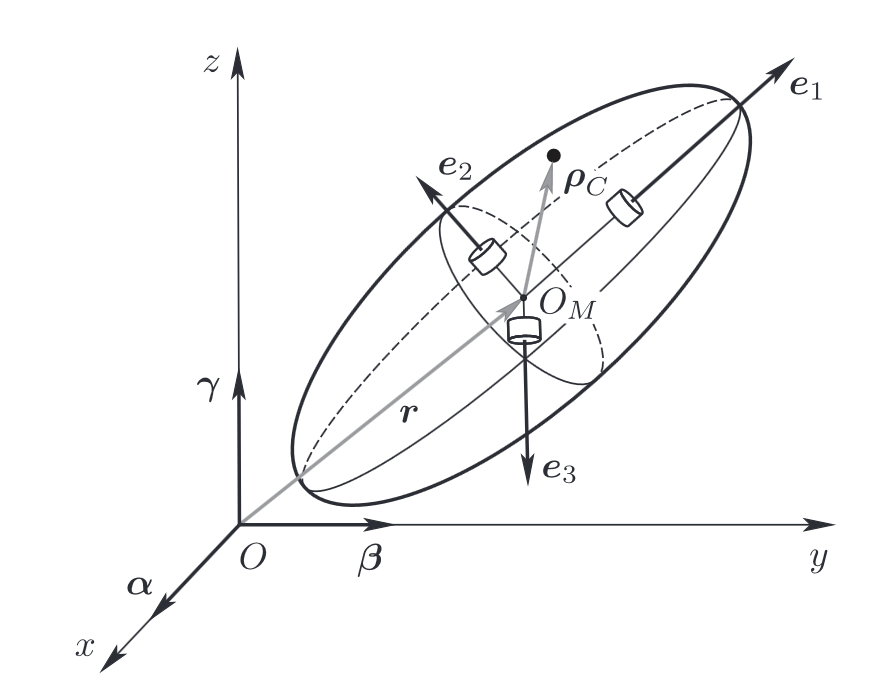
\includegraphics[height=0.8\linewidth]{BPR_Scheme.png} %Shell.eps %BPR_Scheme.png				
				\end{center}
			\end{figure}	
		\end{minipage}
		\hfill
		\begin{minipage}[t]{0.57\linewidth}
			$O x y z$ -- неподвижная система координат;
			
			$O_M e_1 e_2 e_3$ -- подвижная система координат;
			
			$\br = \bigl( x,\, y,\, z \bigr)$ -- координаты геометрического центра оболочки;
			
			${\bal}$, ${\bbe}$, ${\bga}$ -- орты неподвижных осей $O x y z$, спроецированные на подвижные оси $e_1$, $e_2$, $e_3$;

			$\bV$ и ${\bOm}$ -- скорость центра оболочки и его угловая скорость.
			
		\end{minipage}	
	
	Кинематические соотношения и уравнения эволюции $\bigl( \br,\, {\bbQ} \bigr)$:	
	\begin{minipage}{0.47\linewidth}
		%\vspace{-3mm}
		\begin{gather*}
		\dot{{\bal}} = {\bal} \times {\bOm},\, \dot{{\bbe}} = {\bbe} \times {\bOm},\, \dot{{\bga}} = {\bga} \times {\bOm},\\
		\dot{\br} = {\bbQ}^T \bV.
		\end{gather*}	
	\end{minipage}
	\begin{minipage}{0.47\linewidth}
		\vspace{-3mm}
		\begin{gather}
		\bbQ =\begin{pmatrix}
		\alpha _1 & \beta _1 & \gamma _1\\
		\alpha _2 & \beta _2 & \gamma _2\\
		\alpha _3 & \beta _3 & \gamma _3
		\end{pmatrix}\nonumber \in SO(3)
		\end{gather}
	\end{minipage}
	
	Уравнения движения рассматриваемой системы имеют вид классических уравнений Кирхгофа
	\begin{gather}
	\frac{d}{dt} \biggl( \frac{\partial T}{\partial \bV} \biggr) + {\bOm} \times \frac{\partial T}{\partial \bV}=0, \quad \frac{d}{dt}\biggl( \frac{\partial T}{\partial {\bOm}} \biggr) + {\bOm} \times \frac{\partial T}{\partial {\bOm}} + \bV \times \frac{\partial T}{\partial \bV} = 0 \nonumber
	\end{gather}
	
\end{frame}



\begin{frame}
\frametitle{Уравнения движения}
\begin{itemize}
	
	\item После подстановки кинетической энергии в уравнения Кирхгоффа система уравнений, описывающих движение имеет вид
	\begin{gather*}
	\begin{split}
	{\bbC} \dot{\bV} + {\bbB} \dot{{\bOm}} = & \bigl( {\bbC} \bV + {\bbB} {\bOm} \bigr) \times {\bOm},\\
	{\bbB}^T \dot{\bV} + {\bbI} \dot{{\bOm}} + \dot{\bK}(t) = & \bigl( {\bbB}^T \bV + {\bbI} {\bOm} + \bK(t) \bigr) \times {\bOm} + \bigl( {\bbC} \bV + {\bbB} {\bOm} \bigr) \times \bV = 0 
	\end{split}
	\\
	\begin{gathered}
	\dot{{\bal}} = {\bal} \times {\bOm},\quad \dot{{\bbe}} = {\bbe} \times {\bOm},\quad \dot{{\bga}} = {\bga} \times {\bOm},\quad
	\dot{\br} = {\bbQ}^T \bV.
	\end{gathered}	
	\end{gather*}
	
%	\item Для полного описания движения системы данные уравнения необходимо дополнить уравнениями эволюции переменных $\bigl( \br,\, {\bbQ} \bigr)$%, которые описываются уравнениями Пуассона 
%	и кинематическими соотношениями 
%	\begin{gather*}
%	\dot{{\bal}} = {\bal} \times {\bOm},\quad \dot{{\bbe}} = {\bbe} \times {\bOm},\quad \dot{{\bga}} = {\bga} \times {\bOm},\quad
%	\dot{\br} = {\bbQ}^T \bV.
%	\end{gather*}
	
	\item Уравнения в форме импульса и момента импульса:
	\begin{gather*}
	\label{motion_ham}
	\dot{\bP}= \bP \times {\bOm}, \quad \dot{\bM} = \bM \times {\bOm} + \bP \times \bV,
	\end{gather*}	
	где $\bP = \dfrac{\partial T}{\partial \bV}$ и $\bM = \dfrac{\partial T}{\partial {\bOm}}$ 
	
	\item Связь $\bV$ и ${\bOm}$ с $ \bP $ и $\bM  $:
	\begin{gather}
	\label{p_and_M}
	\begin{split}
	\bP = & {\bbC} \bV + {\bbB} {\bOm},\, \quad \bM = {\bbB}^T \bV + {\bbI} {\bOm} + \bK(t),\\
	\bV = & {\bbC}^{-1} \bigl( \bP - {\bbB} {\bOm} \bigr),\, \quad {\bOm} = \bigl({\bbI} - {\bbB}^T {\bbC}^{-1} {\bbB} \bigr)^{-1} \bigl( \bM - \bK(t) - {\bbB}^T {\bbC}^{-1} \bP \bigr)
	\end{split}\nonumber
	\end{gather}
	
\end{itemize}
\end{frame}

\begin{frame}
\frametitle{Первые интегралы}
\begin{itemize}
	
	

	
	\item Уравнения допускают шесть геометрических интегралов движения:
	\begin{gather}
	{\bal}^2={\bbe}^2={\bga}^2=1, \quad \bigl({\bal},\, {\bbe} \bigr) = \bigl({\bal},\, {\bga} \bigr) = \bigl({\bbe},\, {\bga} \bigr) = 0\nonumber
	\end{gather}
	
	\item Уравнения в форме импульса и момента допускают еще шесть интегралов
	\begin{gather*}
	(\bP,\, {\bal}),\, (\bP,\, {\bbe}),\, (\bP,\, {\bga}),\, (\bM + \br \times \bP,\, {\bal}),\, (\bM + \br \times \bP,\, {\bbe}),\, (\bM + \br \times \bP,\, {\bga}). \label{integrals}
	\end{gather*}
	
	\item В случае движения из состояния покоя первые интегралы приобретают особенно простой вид:
	\begin{gather}
	\bP = 0, \quad \bM = 0 \nonumber,
	\end{gather}
	а выражения для скоростей:
	\begin{gather}
	\bV = - \bbC^{-1} \bbB \bOm,  \nonumber \quad
	\bOm = \widetilde{\bbI} \bK(t). \nonumber 	
	\end{gather}
	
	\item Уравнения движения на нулевом уровне
	\begin{gather*}
	\dot{{\bal}} = {\widetilde{\bbI} \bK(t)}  \times {\bal},\quad
	\dot{{\bbe}} = {\widetilde{\bbI} \bK(t)}  \times {\bbe},\quad
	\dot{{\bga}} = {\widetilde{\bbI} \bK(t)}  \times {\bga},\\
	\dot{\br} =  {\bbQ}^T \bbC^{-1} \bbB \widetilde{\bbI} \bK(t),
	\end{gather*}
	где $ \bK(t)=\sum \limits_{k=0}^3 i_k \omega_k (t)\bn_k $, $ \widetilde{\bbI} = \bigl(\bbI - \bbB^T \bbC^{-1} \bbB \bigr)^{-1} $.

	
\end{itemize}
\end{frame}

\begin{frame}[shrink=10]
\frametitle{Исследование управляемости системы}

Представим систему уравнений движения в виде
{\small \begin{gather*}
	\dot{\bq} = \bX_1 (\psi,\, \theta,\, \varphi) \Omega_1 + \bX_2 (\psi,\, \theta,\, \varphi) \Omega_2 + \bX_3 (\psi,\, \theta,\, \varphi) \Omega_3,\\
	\begin{gathered}
	\bX_1 = \left( \dfrac{\sin \varphi}{\sin \theta} ,\, \cos \varphi ,\, -\cot\theta \sin\varphi ,\, 
	\dfrac{ m y_c\alpha_3 }{c_3} - \dfrac{m z_c \alpha_2}{c_2}, \, 
	\dfrac{m y_c \beta_3 }{c_3} - \dfrac{m z_c \beta_2}{c_2} ,\, 
	\dfrac{m y_c \gamma_3 }{c_3} - \dfrac{m z_c \gamma_2}{c_2} \right)^T,\\
	\bX_2 = \left( \dfrac{\cos \varphi}{\sin \theta} ,\, -\sin \varphi ,\, -\cot\theta \cos\varphi ,\, 
	\dfrac{m z_c\alpha_1 }{c_1} - \dfrac{m x_c \alpha_3}{c_3}, \, 
	\dfrac{m z_c \beta_1 }{c_1} - \dfrac{m x_c \beta_3}{c_3} ,\, 
	\dfrac{m z_c \gamma_1 }{c_1} - \dfrac{m x_c \gamma_3}{c_3} \right)^T,\\
	\bX_3 = \left( 0 ,\, 0 ,\, 1 ,\, 
	\dfrac{m x_c \alpha_2 }{c_2} - \dfrac{m y_c \alpha_1}{c_1}, \, 
	\dfrac{m x_c \beta_2 }{c_2} - \dfrac{m y_c \beta_1}{c_1} ,\, 
	\dfrac{m x_c \gamma_2 }{c_2} - \dfrac{m y_c \gamma_1}{c_1} \right)^T,
	\end{gathered}
	\end{gather*}}
где $\bq = (x,\, y,\, z \, \psi,\, \theta,\, \varphi)$ -- вектор обобщенных координат.

%Построим следующие векторные поля:
%\begin{gather*}
%\begin{gathered}
%\bX_{1,2} = \left[ \bX_1,\, \bX_2\right],\quad \bX_{3,1} = \left[ \bX_3,\, \bX_1\right],\quad \bX_{2,3} = \left[ \bX_2,\, \bX_3\right], \\  
%\bX_{1,(2,3)} = \left[ \bX_1,\, \bX_{2,3}\right],\quad \bX_{2,(3,1)} = \left[ \bX_2,\, \bX_{3,1}\right], \quad \bX_{3,(1,2)} = \left[ \bX_3,\, \bX_{1,2}\right],\\
%\end{gathered}
%\end{gather*}
Выберем три набора векторных полей
\begin{gather*}
\begin{gathered}
\Bigl( \bX_1,\, \bX_2,\,\bX_3,\,\bX_{1,2},\,\bX_{2,3},\,\bX_{2,(3,1)},\, \Bigr),\quad
\Bigl( \bX_1,\, \bX_2,\,\bX_3,\,\bX_{2,3},\,\bX_{3,1},\,\bX_{3,(1,2)},\, \Bigr), \\
\Bigl( \bX_1,\, \bX_2,\,\bX_3,\,\bX_{3,1},\,\bX_{1,2},\,\bX_{1,(2,3)},\, \Bigr),
\end{gathered}
\end{gather*}
где $\bX_{i,j} = \left[ \bX_i,\, \bX_j\right]  $.

Условия линейной зависимости векторных полей в указанных наборах имеют вид
\begin{gather*}
\begin{gathered}
x_c(c_2 - c_3) = 0,\quad
y_c(c_3-c_1) = 0, \quad
z_c(c_1-c_2) = 0.
\end{gathered}
\end{gather*}

%Скобка Ли для векторных полей $ \bbs v $ и $ \bbs u $ имеет выражение
%\begin{gather*}
%[\bbs v, \bbs u]_{i}=\sum_{j}v_{j}\frac{\partial u_{i}}{\partial q_{j}}-u_{j}\frac{\partial v_{i}}{\partial q_{j}}
%\end{gather*}

\end{frame}

%\begin{frame}
%\frametitle{Исследование управляемости системы}
%
%Для исследования управляемости представим систему уравнений движения в виде
%\begin{gather*}
%\dot{\bq} = \bX_1 (\psi,\, \theta,\, \varphi) \Omega_1 + \bX_2 (\psi,\, \theta,\, \varphi) \Omega_2 + \bX_3 (\psi,\, \theta,\, \varphi) \Omega_3,
%\end{gather*}
%где $\bq = (x,\, y,\, z \, \psi,\, \theta,\, \varphi)$ -- вектор обобщенных координат. \\
%
%\vspace{4 mm}
%
%\textbf{Теорема.} Система вида $\dot{\bq} = \sum_{i=1}^{M}\bX_i(\bq) u_i$, управляема в некоторой области $N$-мерного пространства, если среди векторных полей $\bX_i$ и всевозможных их коммутаторов $\bX_{i,j} = [\bX_i,\, \bX_j]$, $\bX_{k,(i,j)} = [\bX_k,\, \bX_{i,j}]$, \ldots, составленных последовательными применениями скобки Ли $[\cdot,\, \cdot]$, найдется $N$ линейно независимых в каждой точке области.\\
%
%Построим следующие векторные поля:
%\begin{gather*}
%\begin{gathered}
%\bX_{1,2} = \left[ \bX_1,\, \bX_2\right],\quad \bX_{3,1} = \left[ \bX_3,\, \bX_1\right],\quad \bX_{2,3} = \left[ \bX_2,\, \bX_3\right], \\  
%\bX_{1,(2,3)} = \left[ \bX_1,\, \bX_{2,3}\right],\quad \bX_{2,(3,1)} = \left[ \bX_2,\, \bX_{3,1}\right], \quad \bX_{3,(1,2)} = \left[ \bX_3,\, \bX_{1,2}\right],\\
%\end{gathered}
%\end{gather*}
%Выберем три набора векторных полей
%\begin{gather*}
%\begin{gathered}
%\Bigl( \bX_1,\, \bX_2,\,\bX_3,\,\bX_{1,2},\,\bX_{2,3},\,\bX_{2,(3,1)},\, \Bigr),\quad
%\Bigl( \bX_1,\, \bX_2,\,\bX_3,\,\bX_{2,3},\,\bX_{3,1},\,\bX_{3,(1,2)},\, \Bigr), \\
%\Bigl( \bX_1,\, \bX_2,\,\bX_3,\,\bX_{3,1},\,\bX_{1,2},\,\bX_{1,(2,3)},\, \Bigr),
%\end{gathered}
%\end{gather*}
%
%
%\end{frame}
%
%\begin{frame}
%\frametitle{Исследование управляемости системы}
%
%Условия линейной зависимости векторных полей в указанных наборах имеют вид
%\begin{gather*}
%\begin{gathered}
%x_c(c_2 - c_3) = 0,\quad
%y_c(c_3-c_1) = 0, \quad
%z_c(c_1-c_2) = 0.
%\end{gathered}
%\end{gather*}
%
%Движение в идеальной жидкости однородной оболочки, имеющей форму эллипсоида, вполне управляемо с помощью вращения трех роторов, за исключением трех частных случаев:
%\begin{enumerate}
%	\item система “ оболочка + роторы” уравновешена;
%	\item оболочка имеет сферическую форму;
%	\item оболочка имеет форму эллипсоида вращения, а центра масс всей системы	расположен на оси вращения.
%\end{enumerate}

%Добавим к оболочке в виде эллипсоида винтовые лопасти. Так, объект будет представлять из себя трехлопастной винт.
%
%\end{frame}







%\begin{frame}
%\frametitle{Создание прототипа робота}
%
%При создании робота имеются следующие технические требования и ограничения:
%\begin{itemize}
%	\item Перпендикулярность роторов.
%	\item Для создания максимального эффекта момент инерции роторов должен быть максимальным --- ограничивается выбранными двигателями.
%	\item Центр масс всей системы должен быть расположен максимально близко к геометрическому центру эллипсоида.
%	\item Форма робота в виде винтового тела --- эллипсоид вращения + лопасти.
%	\item Размер оболочки робота не должен превышать 200х300 мм --- ограничение литьевой машины. 
%	\item Диаметр роторов --- ограничивается размерами оболочки.	
%\end{itemize}
%
%
%
%\end{frame}






\begin{frame}
\frametitle{Разработка прототипа робота}

Конструкция и корпусные элементы экспериментальной модели безвинтового подводного робота.

\begin{minipage}[ht]{0.33\linewidth}
	\vspace{-27mm}
	\centering{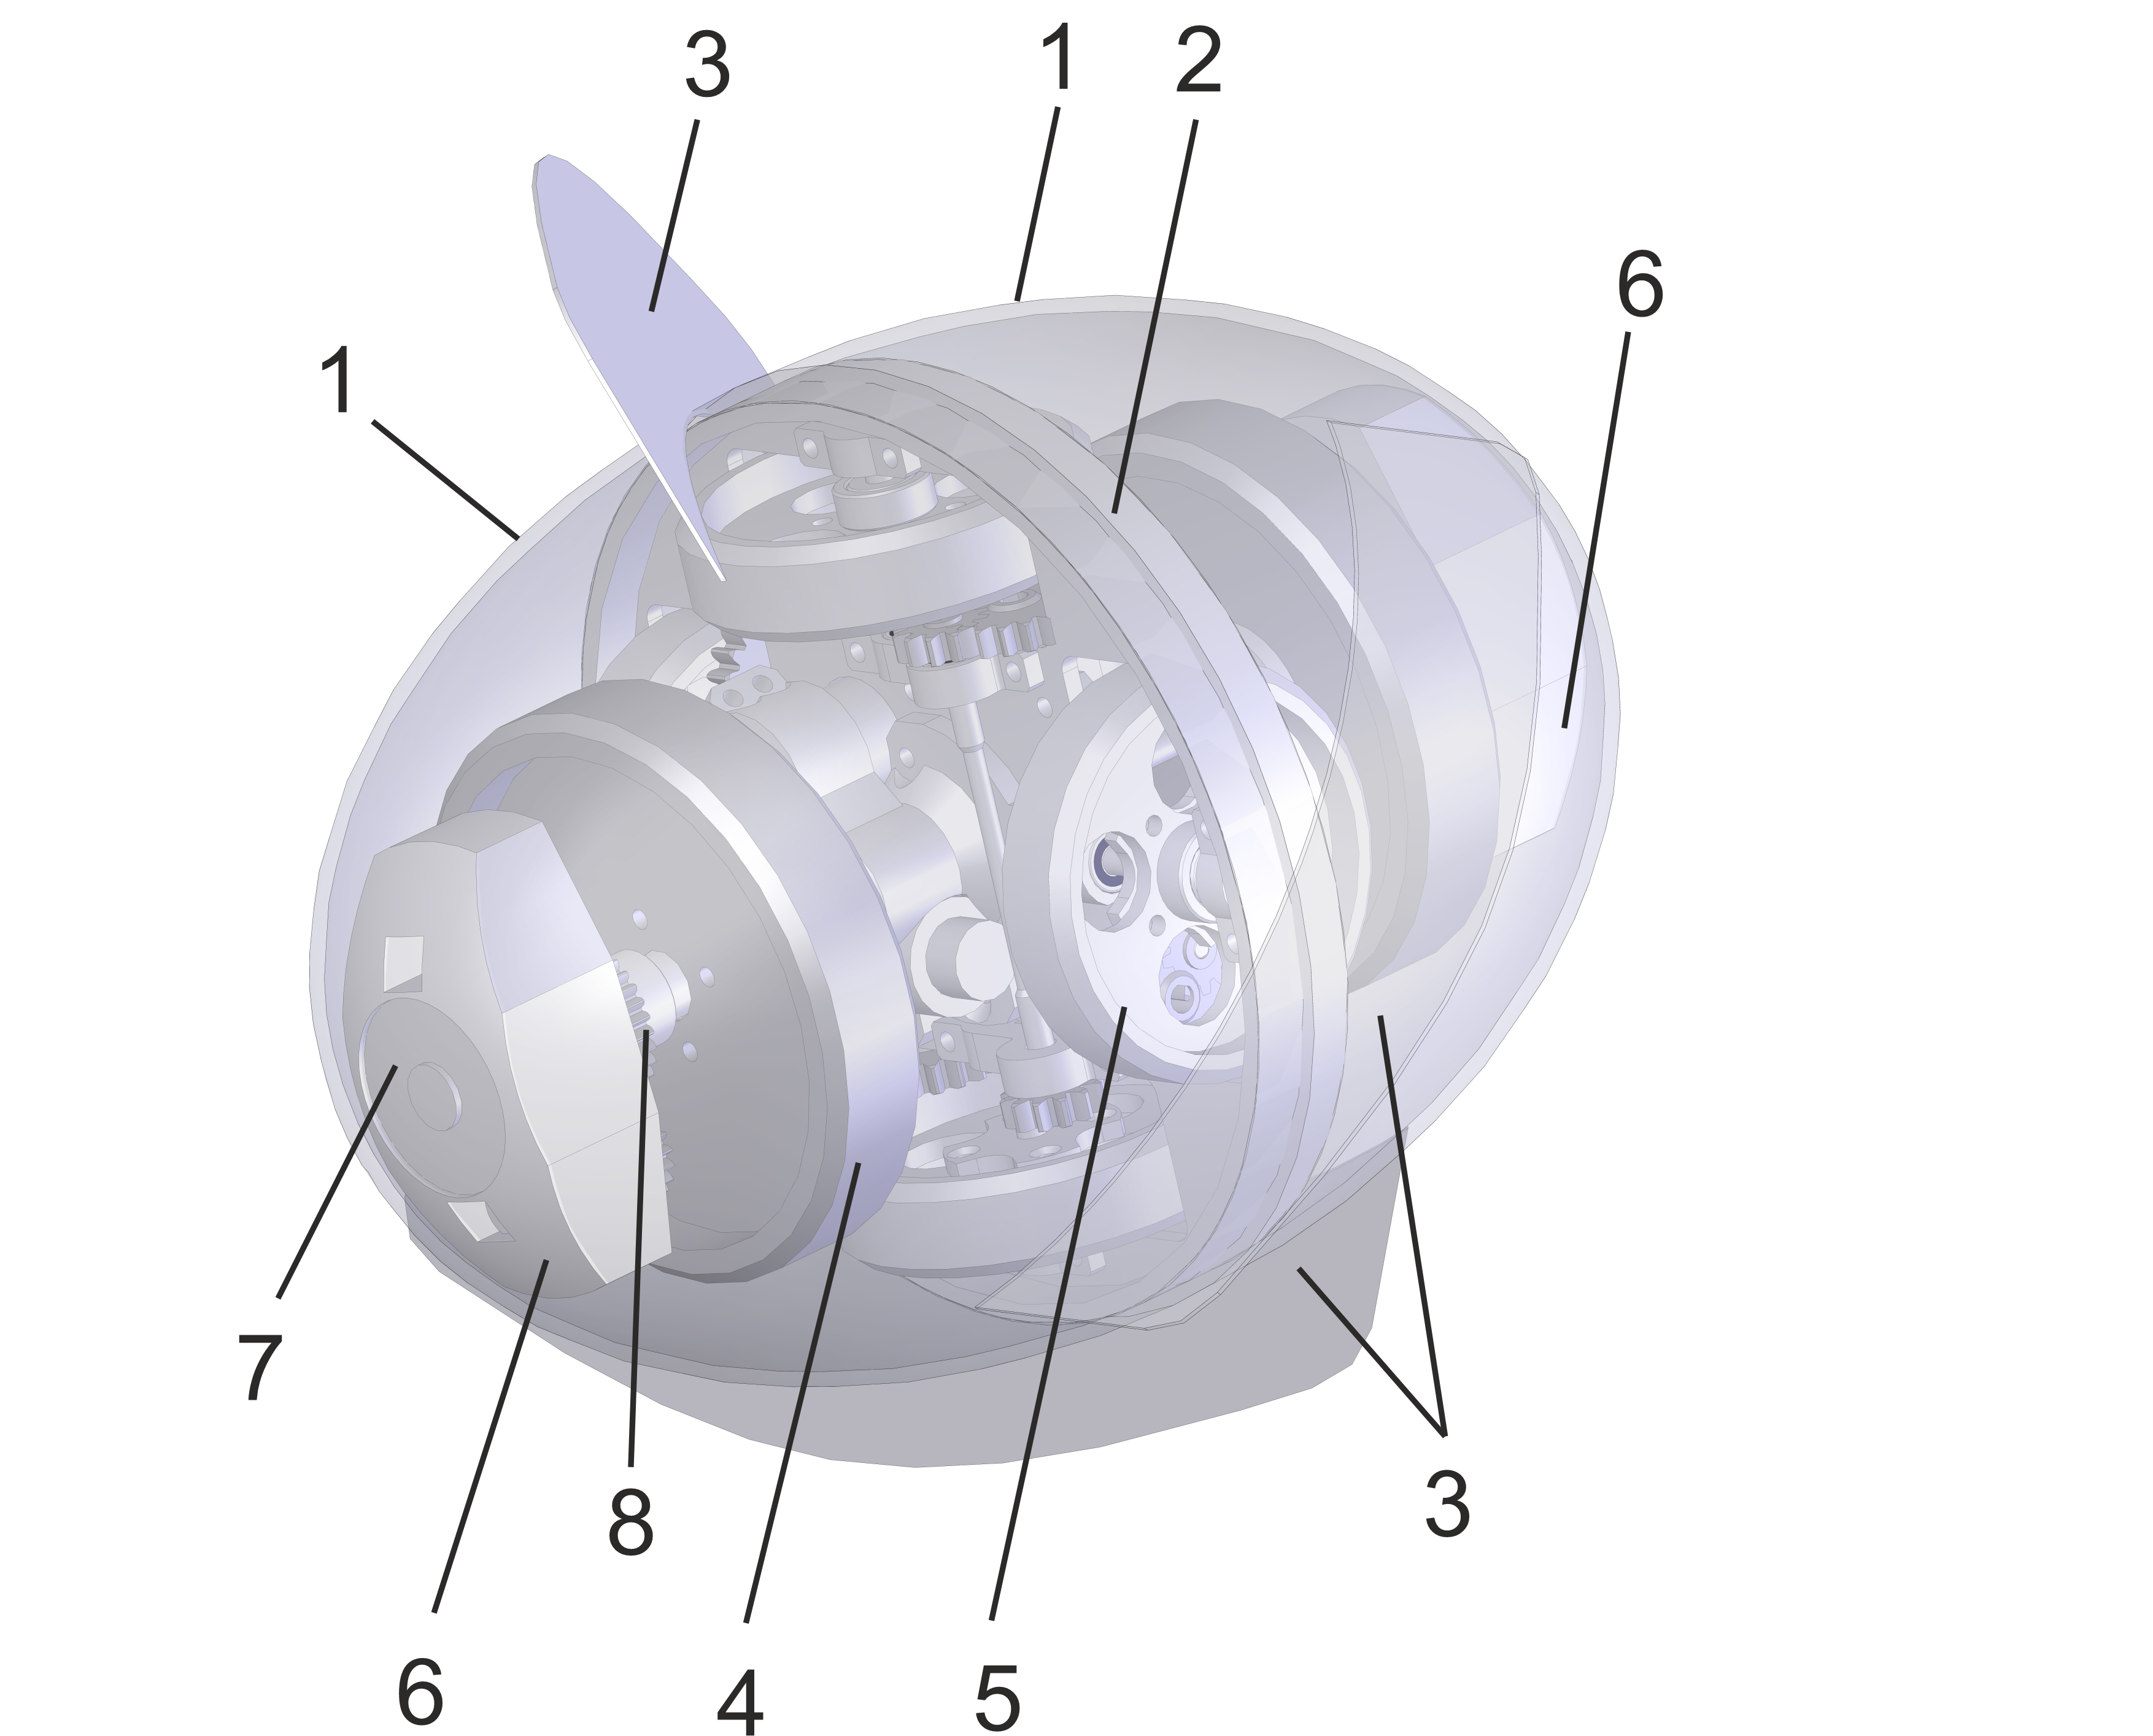
\includegraphics[height=35mm]{BPR_ScrewModel.png} \\}
	\vspace{3mm}
	\centering{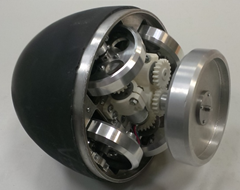
\includegraphics[width=0.9\linewidth]{Photo_BPR3.png} }
\end{minipage}
\hfill
\begin{minipage}[t]{0.63\linewidth}
	\centering{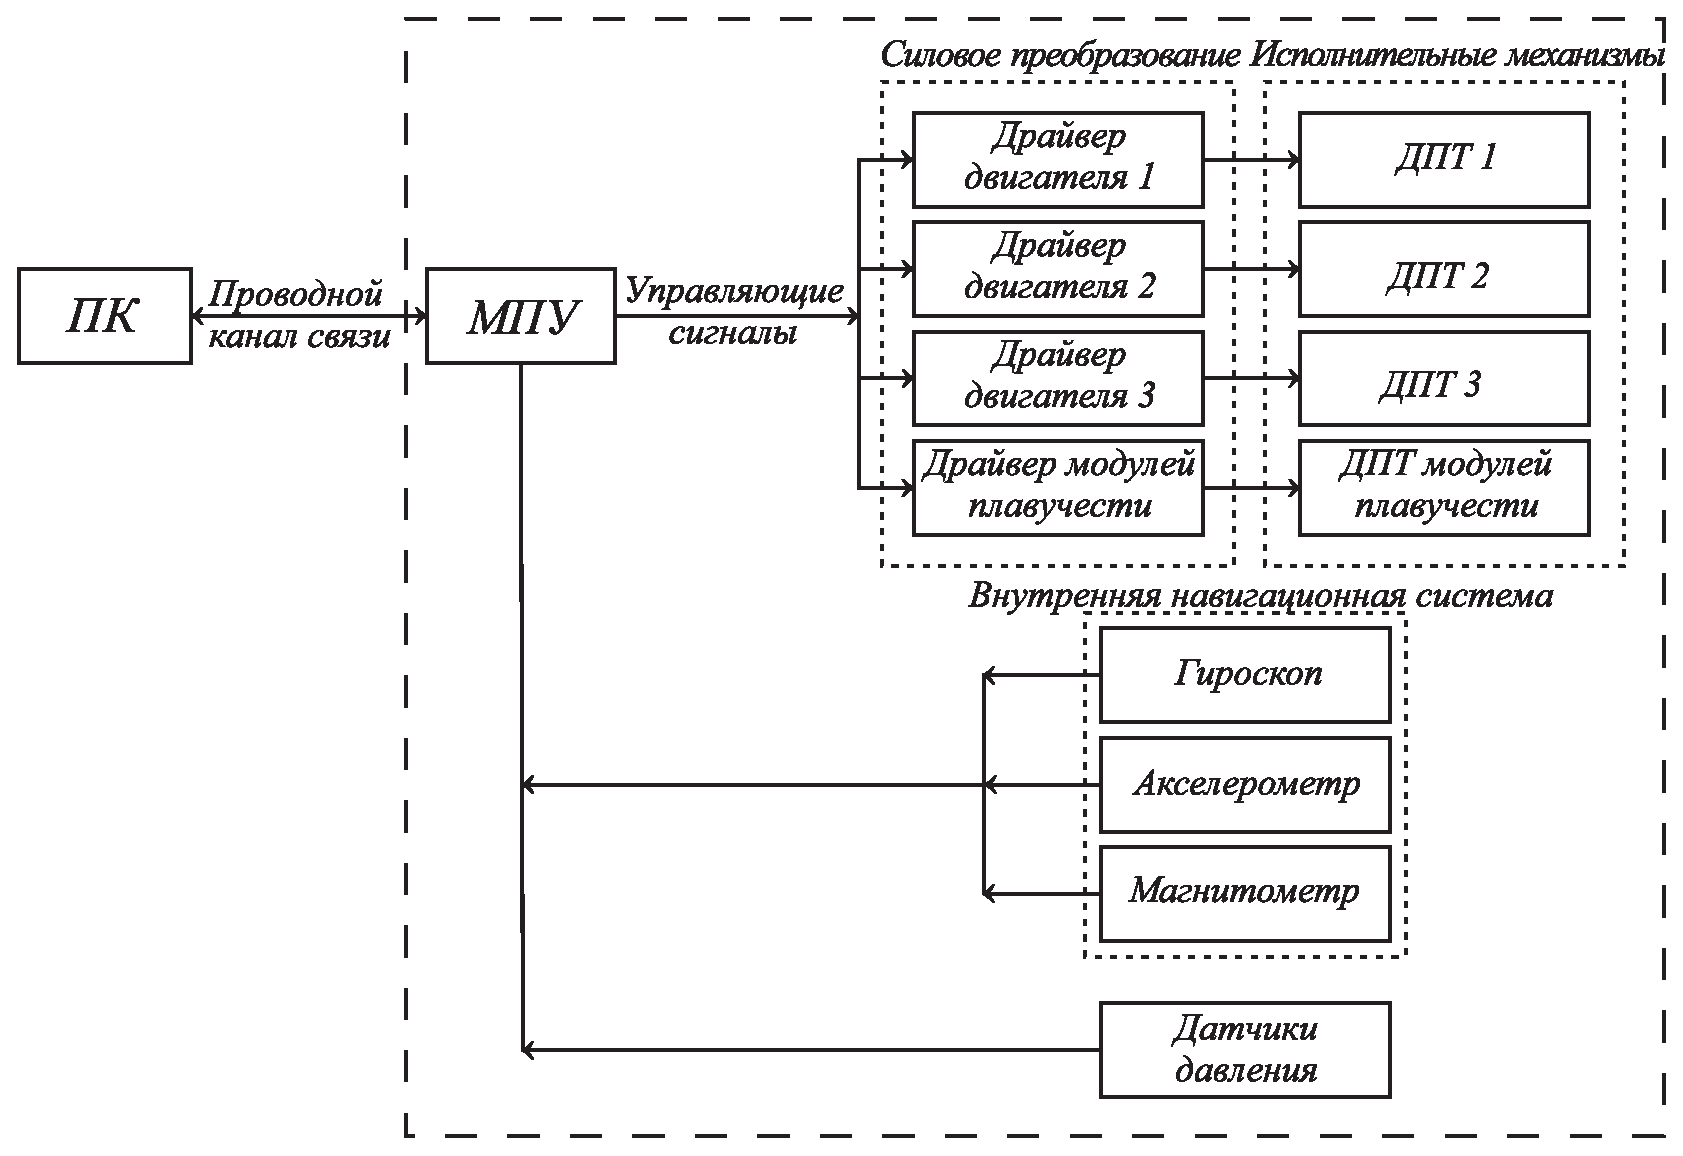
\includegraphics[width=1\linewidth]{StrSchemeBPR.eps} }
	
	\begin{table}
		\centering
		{\begin{tabular}{@{}lc@{}}\hline
				Параметр & Значение \\
				\hline
				Размеры & 300x200x200 мм \\
				Масса оболочки  & 2.923 кг \\
				Масса большого ротора & 0.903 кг \\
				Масса малого ротора & 0.337 кг \\				
				\hline
			\end{tabular}
		}
	\end{table}
\end{minipage}

\end{frame}



%\begin{frame}
%\frametitle{Результаты моделирования}
%%\begin{itemize}
%%	\item Борисов А. В., Ветчанин Е. В., Килин А. А., Управление движением трехосного эллипсоида в жидкости с помощью роторов, Математические заметки, 2017, т. 102, № 4, с. 503-513
%%	\item В работе описаны комбинации управляющих воздействий, которые позволяют реализовать неограниченное движение в произвольном направлении.
%%	
%%	Движение тела представляет собой стационарное винтовое движение с постоянной угловой и линейной скоростями. 
%%\end{itemize}
%
%
%Для решения уравнений движения необходимо:
%\begin{itemize}
%	\item Определить значения тензоров присоединенных масс и присоединенных моментов инерции. 
%	%Для робота в форме эллипсоида вращения данные коэффициенты можно расчитать используя справочные материалы.
%	Для робота винтовой формы коэффициенты расчитывались с помощью программных продуктов SALOME (генерация сетки) и OpenFOAM (численные расчеты).
%	\item Определить значения моментов инерции. Для робота разработанной конструкции моменты инерции определялись с помощью программного продукта SolidWorks.	
%\end{itemize}
%
%Рассмотрим движение тела при постоянных скоростях вращения роторов $\bbs\omega = (\omega_1, \omega_2, \omega_3)^T$.
%
%а) $\omega_1=10$ рад/с, $\omega_2=0$, $\omega_3=0$. б) $\omega_1=0$, $\omega_2=10$ рад/с, $\omega_3=0$. 
%
%в) $\omega_1=10$ рад/с, $\omega_2=10$ рад/с, $\omega_3=0$.
%
%\begin{minipage}[t]{0.3\linewidth}
%	\center{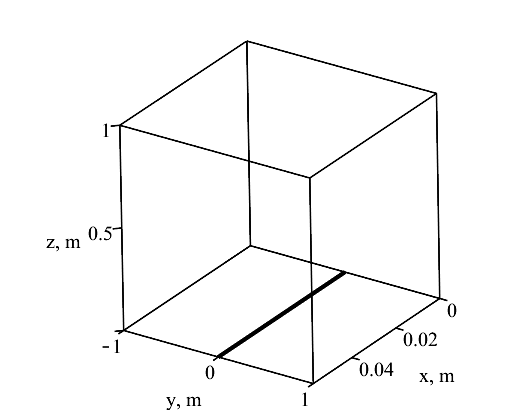
\includegraphics[width=0.95\linewidth]{ModelTrBPR1_.png} \\ а)}
%\end{minipage}
%\hfill
%\begin{minipage}[t]{0.3\linewidth}
%	\center{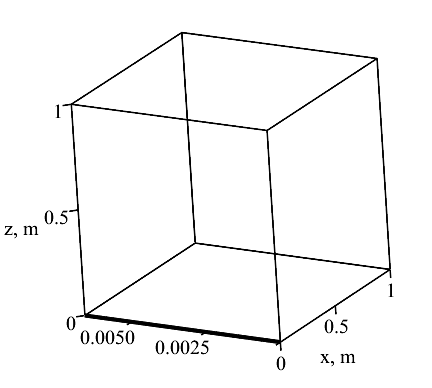
\includegraphics[width=0.95\linewidth]{ModelTrBPR2_.png} \\ б)}
%\end{minipage}
%\hfill
%\begin{minipage}[t]{0.3\linewidth}
%	\center{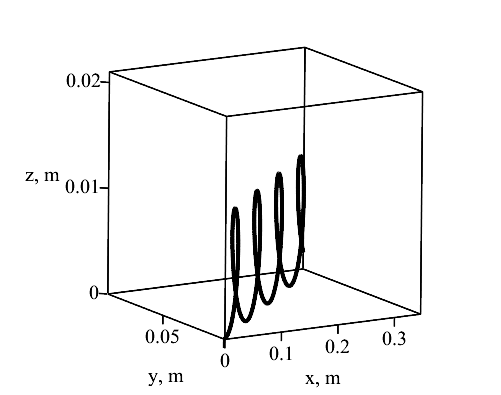
\includegraphics[width=1\linewidth]{ModelTrBPR12_.png} \\ в)}
%\end{minipage}


%\end{frame}

%\begin{frame}
%\frametitle{Система управления}
%В полученных математических моделях управление роторами задается в виде вектора внутреннего гиростатического момента $\bK$. Для управления отдельным двигателем разработана следующая схема
%
%\begin{figure}[h]
%	\centering
%	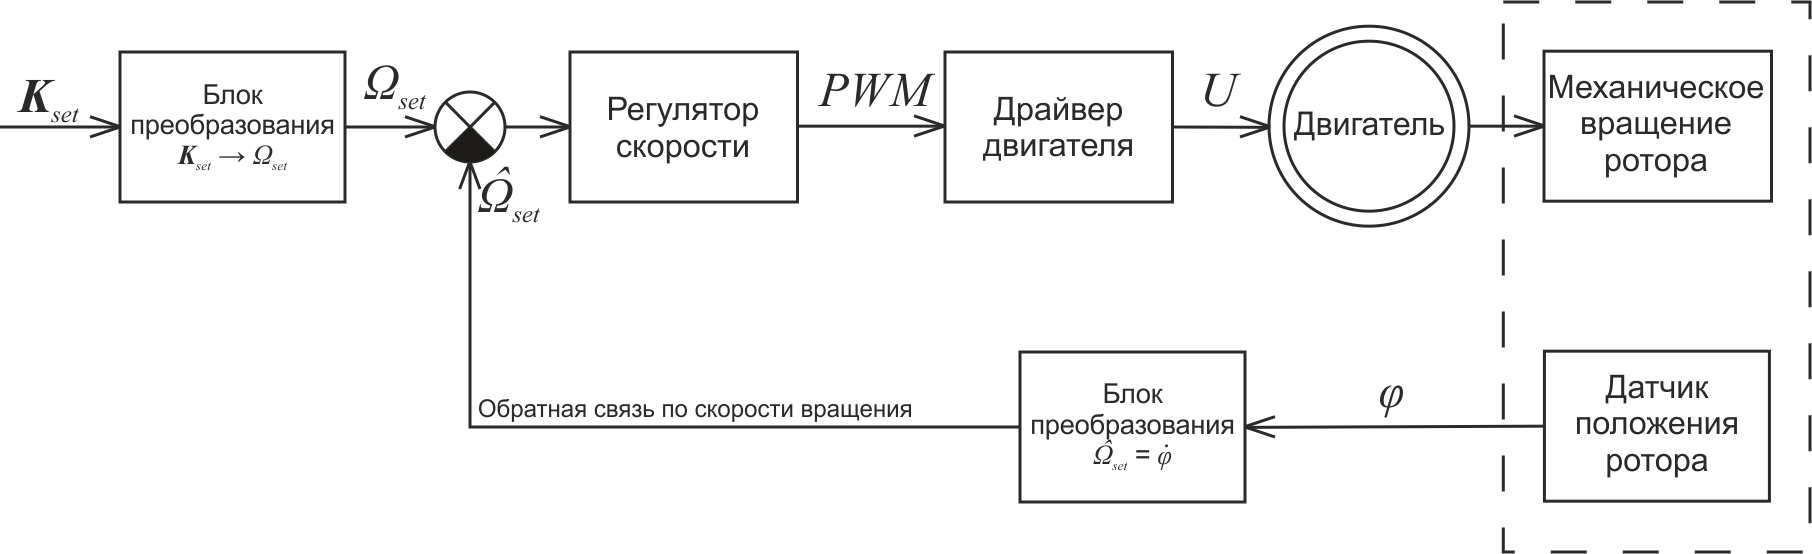
\includegraphics[width=0.9\linewidth]{Control_system.png}%
%\end{figure}
%
%Схема управления отдельным двигателем, где $\bK_{set}$ -- вектор внутреннего гиростатического момента; $\bOm_{set}$ -- угловая скорость вращения двигателя; $\hat{\bOm}_{set}$ -- фактическая скорость вращения двигателя; $PWM$ -- широтно-импульсная модуляция, рассчитаная для заданной скорости вращения; $U$ -- напряжение, подаваемое на двигатель; $\varphi$ -- фактическое положение ротора
%
%\end{frame}



%\begin{frame}
%\frametitle{Экспериментальные исследования}
%1.	Вращение пары больших роторов. $K = (2i_1\omega_{max}, 0, 0)$.
%
%
%	\begin{minipage}[t]{0.3\linewidth}
%		\center{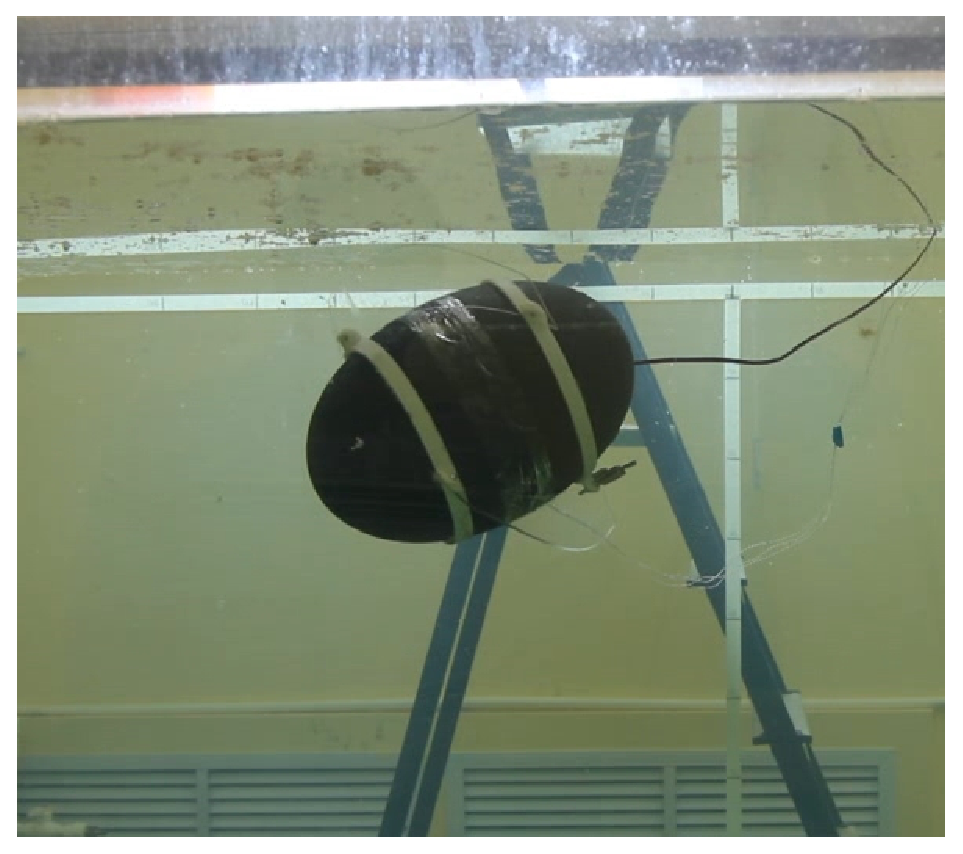
\includegraphics[width=0.7\linewidth]{exp11.eps} \\ а)}
%	\end{minipage}
%	\hfill
%	\begin{minipage}[t]{0.3\linewidth}
%		\center{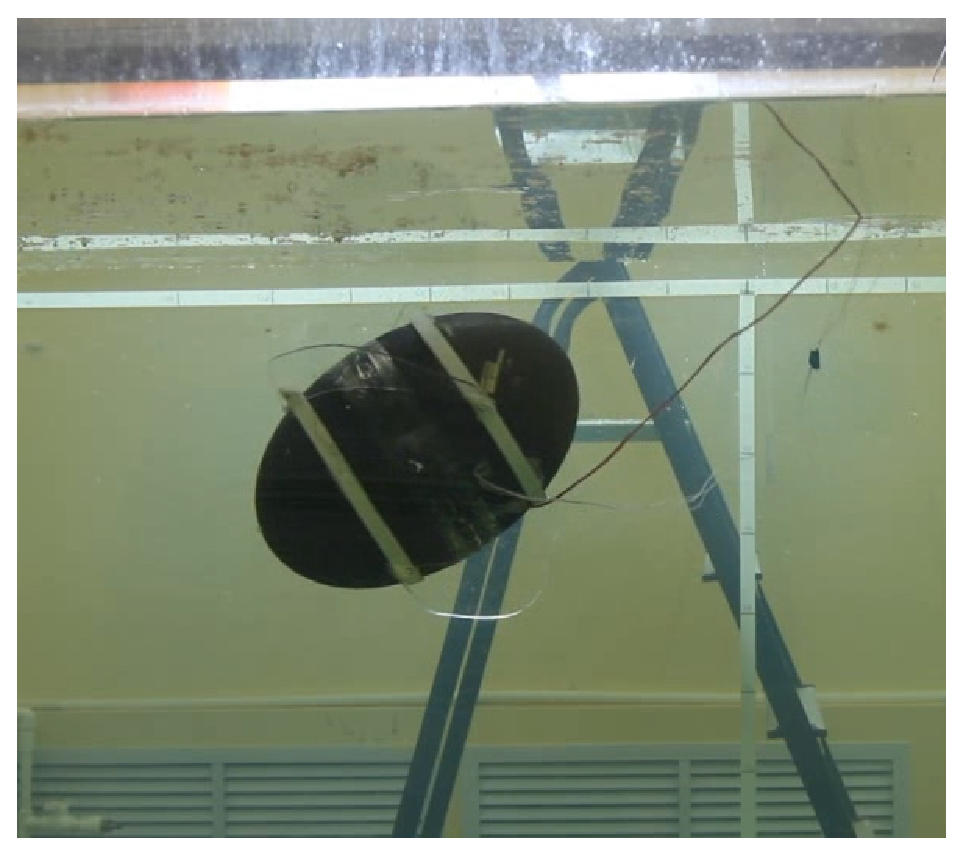
\includegraphics[width=0.7\linewidth]{exp12.eps} \\ б)}
%	\end{minipage}
%	\hfill
%	\begin{minipage}[t]{0.3\linewidth}
%		\center{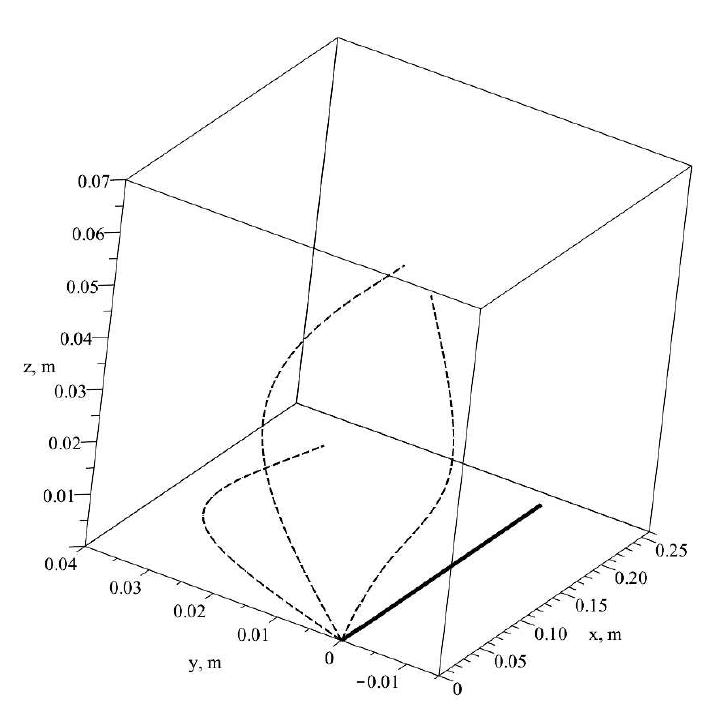
\includegraphics[width=0.8\linewidth]{Exp_BPR_1.png} \\ в)}
%	\end{minipage}
%
%
%Положение робота а) в начальный момент времени и б) момент времени t=3 секунды от начала движения; в) теоретическая (сплошная линия) и экспериментальные (штриховые линии) траектории движения безвинтового подводного робота 
%
%\begin{table}[h]
%	\centering
%	\begin{tabular}{|c|c|c|c|c|c|c|c|}
%		\hline
%		& $\Delta x$, м & $\Delta y$, м & $\Delta z$, м & $|\br_t|$, м & $\Delta \theta$ & $\Delta \psi$ & $\Delta \varphi$ \\ \hline
%		Теория & $0.275$ & $0$ & $0$ & $0.275$ & $ 0^{\circ}$ & $ 0^{\circ}$ & $ 738.2^{\circ}$ \\ \hline
%		Эксперимент & $0.115$  & $0.010$ & $0.055$ & $0.128$ & $ 4^{\circ} $ & $ 10^{\circ} $ & $ 121^{\circ} $  \\
%		\hline
%	\end{tabular}
%\end{table}
%
%\end{frame}
%
%
%\begin{frame}
%\frametitle{Экспериментальные исследования}
%2.	Вращение одной пары малых роторов. $K = (0, 2i_2\omega_{max}, 0)$. 
%
%
%	\begin{minipage}[h]{0.3\linewidth}
%		\center{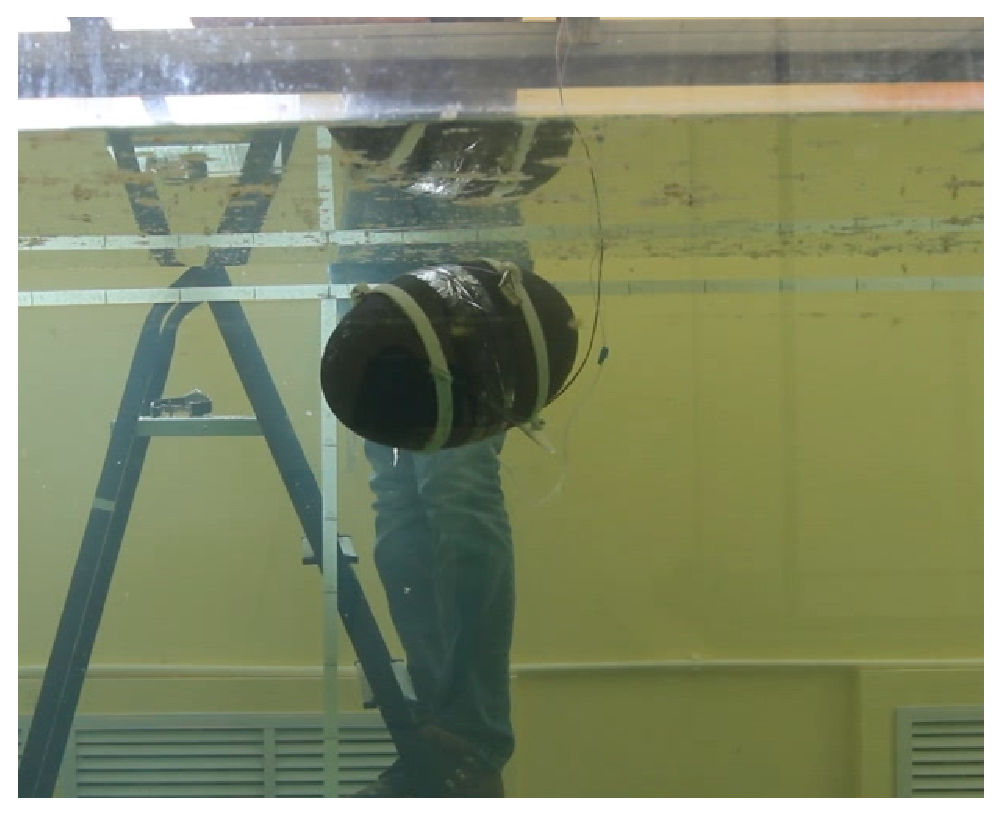
\includegraphics[width=0.7\linewidth]{exp21.eps} \\ а)}
%	\end{minipage}
%	\hfill
%	\begin{minipage}[h]{0.3\linewidth}
%		\center{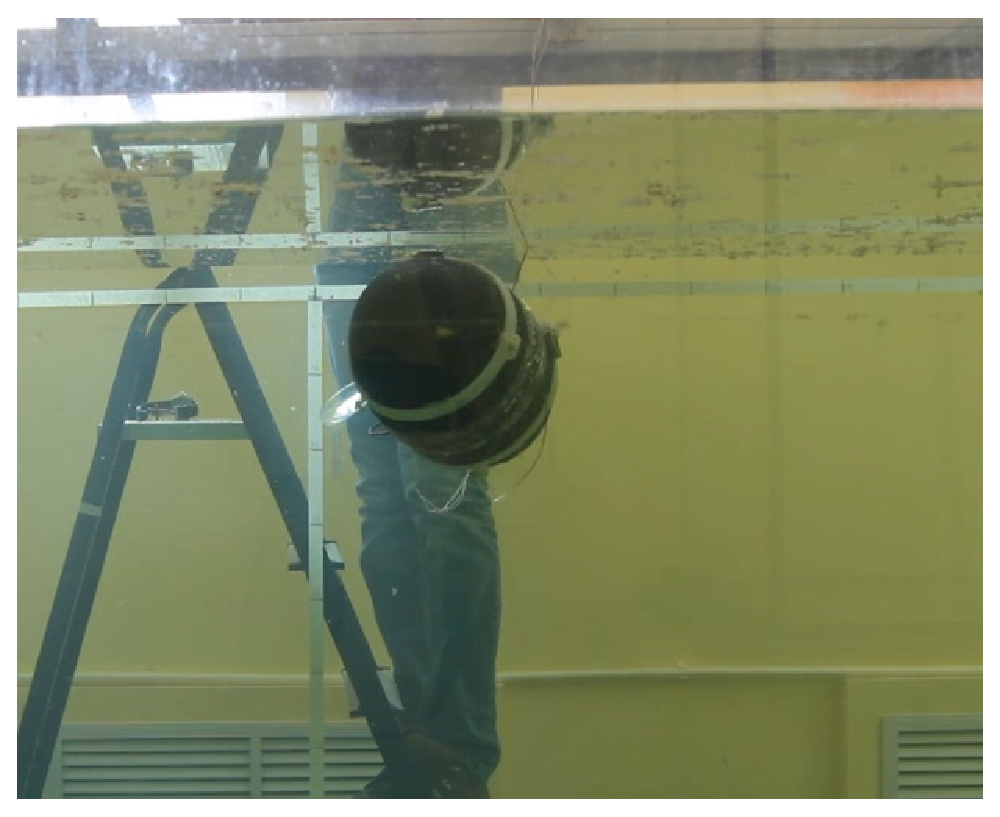
\includegraphics[width=0.7\linewidth]{exp22.eps} \\ б)}
%	\end{minipage}
%	\hfill
%	\begin{minipage}[h]{0.3\linewidth}
%		\center{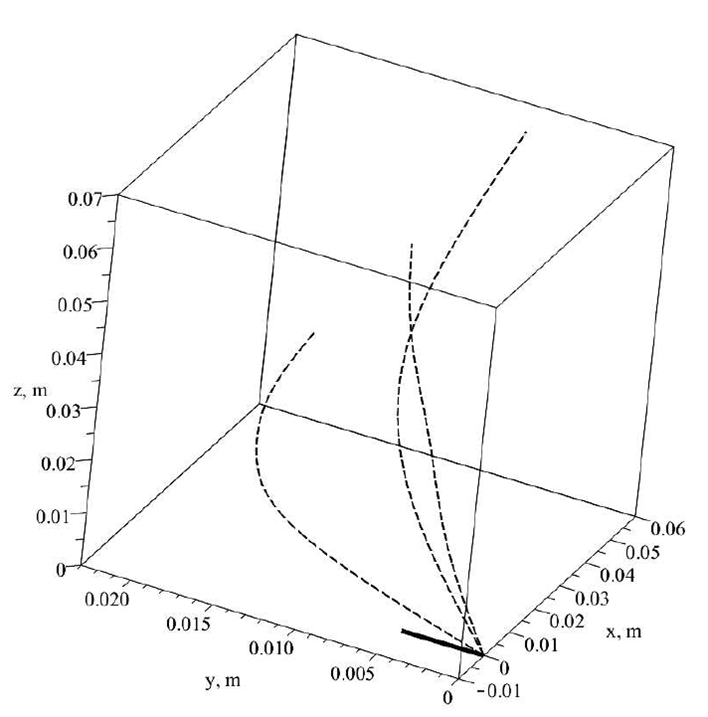
\includegraphics[width=0.8\linewidth]{Exp_BPR_2.png} \\ в)}
%	\end{minipage}
%
%
%Положение робота а) в начальный момент времени и б) момент времени t=3 секунды от начала движения; в) теоретическая (сплошная линия) и экспериментальные (штриховые линии) траектории движения безвинтового подводного робота 
%
%\begin{table}[h]
%	\centering
%	\begin{tabular}{|c|c|c|c|c|c|c|c|}
%		\hline
%		& $\Delta x$, м & $\Delta y$, м & $\Delta z$, м & $|\br_t|$, м & $\Delta \theta$ & $\Delta \psi$ & $\Delta \varphi$ \\ \hline
%		Теория & $0$ & $0.005$ & $0$ & $0.005$ & $ 35^{\circ}$ & $ 0^{\circ}$ & $ 0^{\circ}$ \\ \hline
%		Эксперимент & $0.054$  & $0.008$ & $0.068$ & $0.087$ & $ 61^{\circ} $ & $ 62^{\circ} $ & $ 10^{\circ} $  \\
%		\hline
%	\end{tabular}
%\end{table}
%
%\end{frame}
%
%
%\begin{frame}
%\frametitle{Экспериментальные исследования}
%3.	Вращение пары больших роторов и одной пары малых роторов. $K = (2i_1\omega_{max}, 2i_2\omega_{max}, 0)$. 
%
%	\begin{minipage}[h]{0.3\linewidth}
%		\center{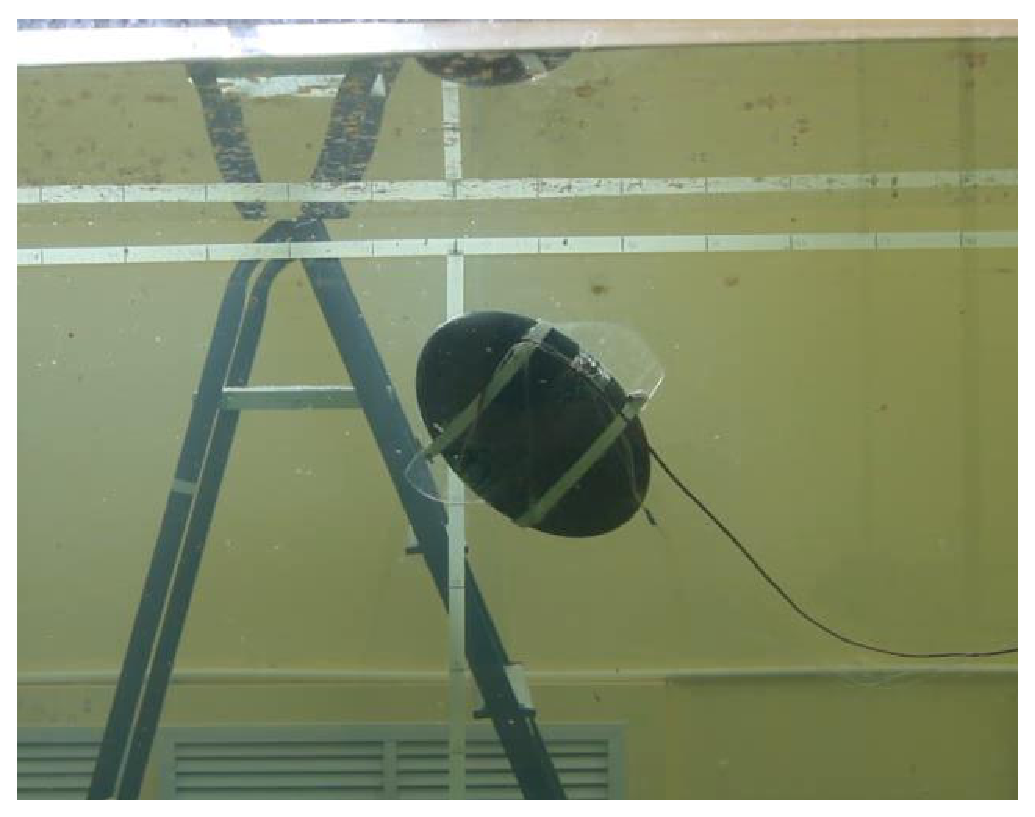
\includegraphics[width=0.7\linewidth]{exp31.eps} \\ а)}
%	\end{minipage}
%	\hfill
%	\begin{minipage}[h]{0.3\linewidth}
%		\center{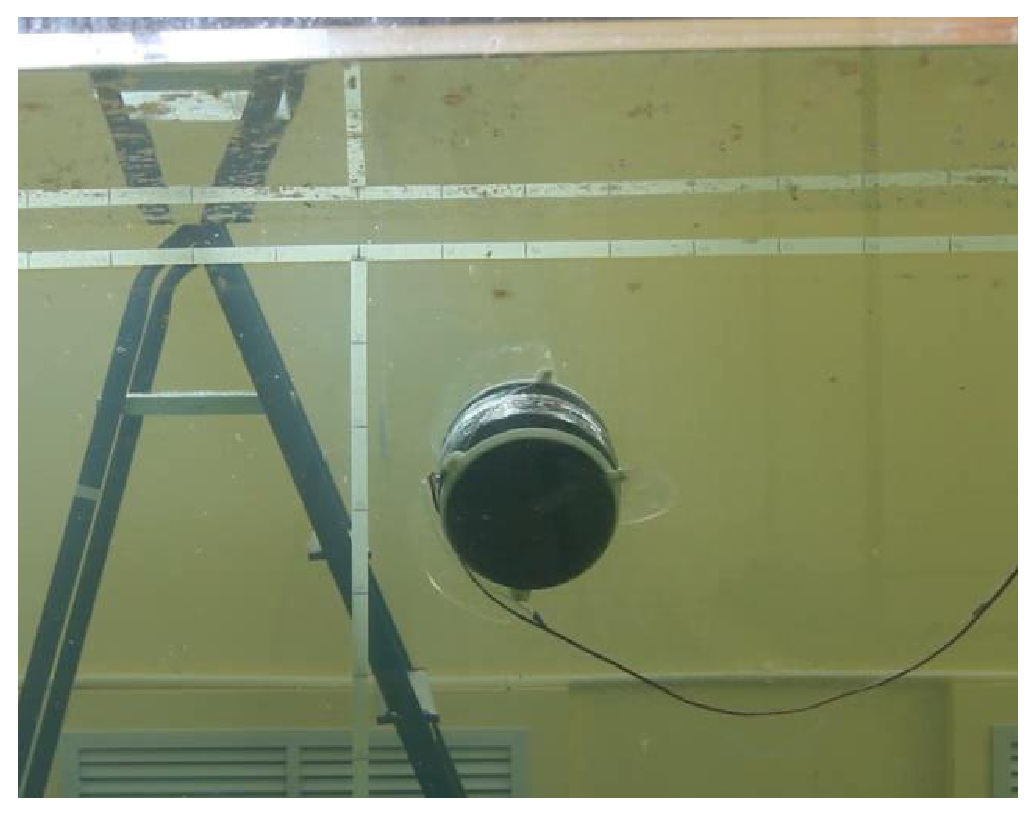
\includegraphics[width=0.7\linewidth]{exp32.eps} \\ б)}
%	\end{minipage}
%	\hfill
%	\begin{minipage}[h]{0.3\linewidth}
%		\center{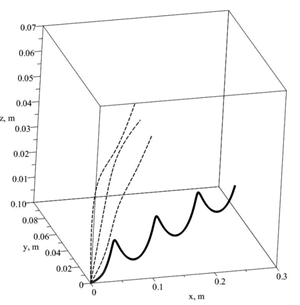
\includegraphics[width=0.8\linewidth]{Exp_BPR_3.png} \\ в)}
%	\end{minipage}
%
%Положение робота а) в начальный момент времени и б) момент времени t=3 секунды от начала движения; в) теоретическая (сплошная линия) и экспериментальные (штриховые линии) траектории движения безвинтового подводного робота 
%
%\begin{table}[h]
%	\centering
%	\begin{tabular}{|c|c|c|c|c|c|c|c|}
%		\hline
%		& $\Delta x$, м & $\Delta y$, м & $\Delta z$, м & $|\br_t|$, м & $\Delta \theta$ & $\Delta \psi$ & $\Delta \varphi$ \\ \hline
%		Теория & $0.275$ & $0$ & $0$ & $0.275$ & $ 35^{\circ}$ & $ 0^{\circ}$ & $ 738.2^{\circ}$ \\ \hline
%		Эксперимент & $0.106$  & $0.050$ & $0.053$ & $0.189$ & $ 17^{\circ} $ & $ 92^{\circ} $ & $ 51^{\circ} $  \\
%		\hline
%	\end{tabular}
%\end{table}
%
%%\begin{center}
%%	$\Delta x_{exp}=0.106\; \mbox{м}, \; \Delta y_{exp}=0.050\; \mbox{м},\; \Delta z_{exp}=0.053\; \mbox{м}, \;$ \\
%%	%\item $|r|=0.129$ м;
%%	$\Delta \theta_{exp}=17^{\circ},\; \Delta \psi_{exp}=90^{\circ},\; \Delta \varphi_{exp}=51^{\circ}.$
%%\end{center}
%
%\end{frame}

\begin{frame}
\frametitle{Экспериментальные исследования}

\begin{minipage}[t]{0.32\linewidth}
	\center{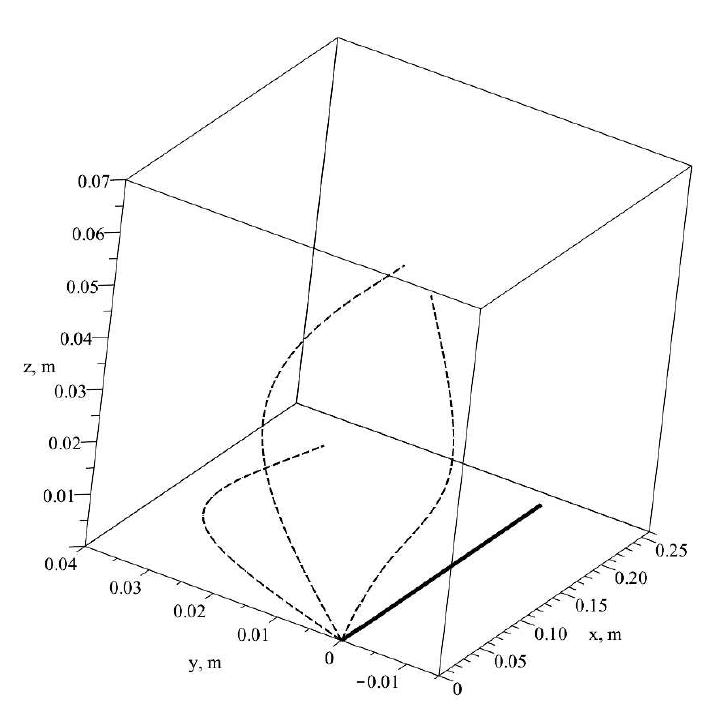
\includegraphics[width=1\linewidth]{Exp_BPR_1.png} \\ а) $K = (2i_1\omega_{m}, 0, 0)$}
\end{minipage}
\hfill
\begin{minipage}[t]{0.32\linewidth}
	\center{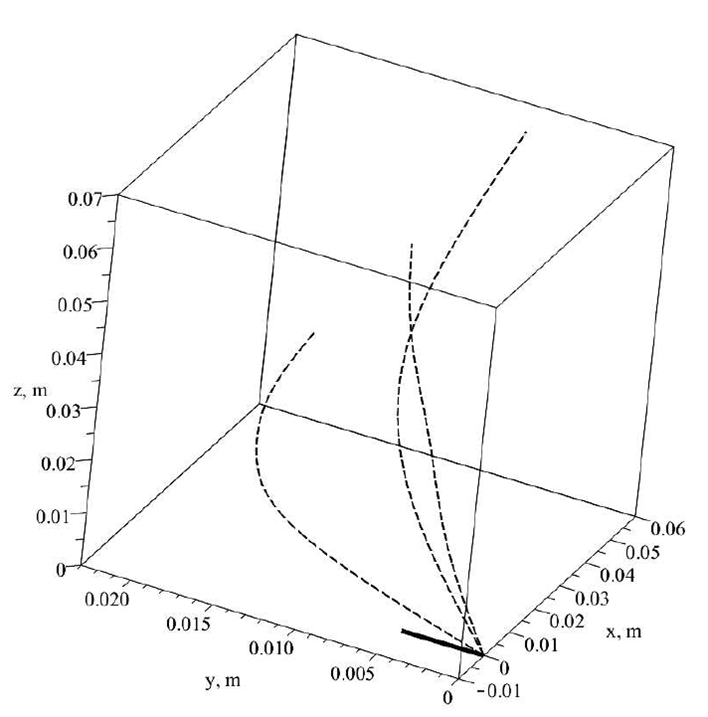
\includegraphics[width=1\linewidth]{Exp_BPR_2.png} \\ б) $K = (0, 2i_2\omega_{m}, 0)$}
\end{minipage}
\hfill
\begin{minipage}[t]{0.32\linewidth}
	\center{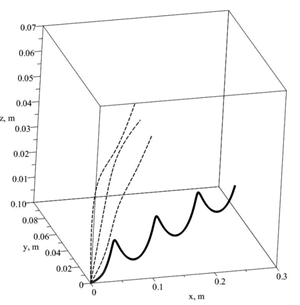
\includegraphics[width=1\linewidth]{Exp_BPR_3.png} \\ в) $K = (2i_1\omega_{m}, 2i_2\omega_{m}, 0)$}
\end{minipage}

\vspace{2mm}

а) Вращение одной пары больших роторов, $|\br_t| = 0.275$ м., $|\br_{exp}| = 0.128$ м.

б) Вращение одной пары малых роторов,  $|\br_t| = 0.005$ м., $|\br_{exp}| = 0.087$ м.

в) Вращение одной пары больших роторов и одной пары малых роторов, $|\br_t| = 0.275$ м., $|\br_{exp}| = 0.189$ м.

\textbf{Выводы.}
\begin{itemize}
	\item Движение только при ускоренном вращении.
	\item Влияние вихрей и взякого сопротивления на траеткорию движения.
	\item Модель качественно описывает движение.
\end{itemize}
\end{frame}

%\begin{frame}
%\frametitle{Выводы}
%
%\begin{itemize}
%	\item	Движение возможно только за счет ускоренного вращения роторов. После достижения максимальной скорости вращения, робот продолжает движение по инерции.
%	\item Разгон маховиков до максимальной скорости занимает определенное время, что не учитывается в теоретической модели. %и вносит свой вклад в траекторию движения безвинтового подводного робота.
%	\item В теоретической модели используется идеализированная модель вязкости, что так же вносит несоответствия теоретической и реальной траектории движения.
%	
%	\item	Движение безвинтового подводного робота сопровождается образованием вихревых структур. Обеспечить безвихревое движение крайне затруднительно.
%	
%	\item Подобную схему и алгоритмы управления в качестве практического применения можно использовать для реализации различных маневров (например, разворот на месте) в управлении подводными роботами.
%	
%	\item \textbf{Модель качественно описывает движение, но на количественное согласование влияет точность определения большого количества параметров. Движение возможно, однако, его эффективность не высока.}
%\end{itemize}
%
%\end{frame}

%\begin{frame}
%\frametitle{Переход}
%
%Ассиметрия тела
%периодическое управление
%Вихри помогают, оболочка с участием вихрей - острая кромка.
%Наводный для простоты.
%
%
%
%
%\end{frame}


\section{Недеформируемый водный робот с внутренним ротором}

\begin{frame}
\frametitle{Недеформируемый водный робот с острой кромкой}

\begin{figure}[!ht]
	\centering
	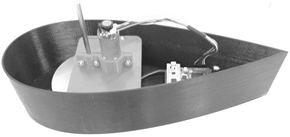
\includegraphics[height=20mm]{Photo_NACA1.png} \hspace{10mm} 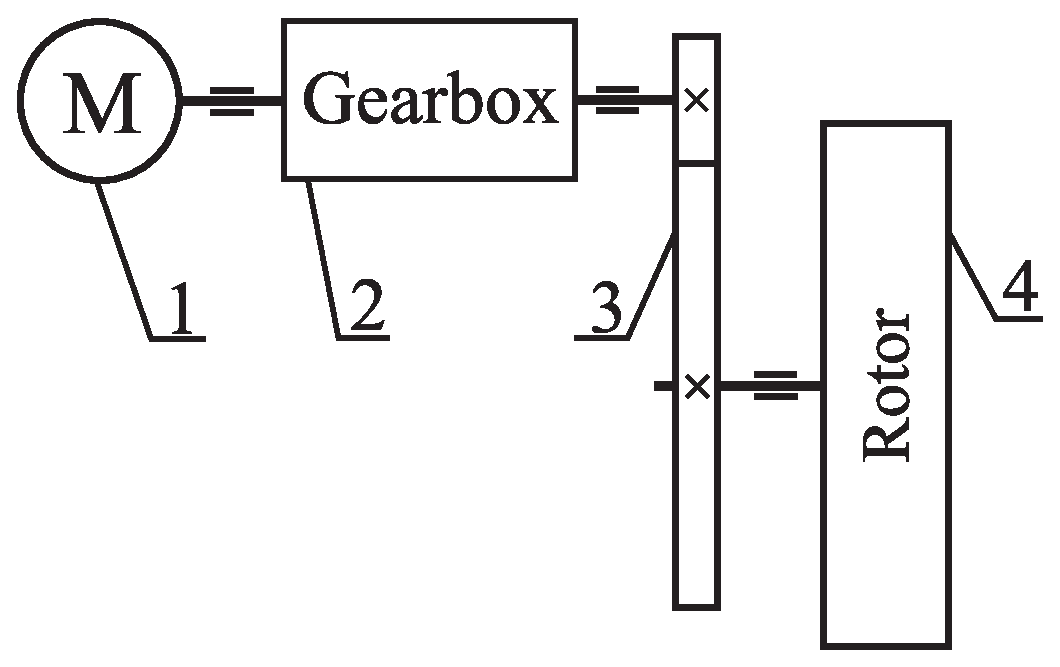
\includegraphics[height=20mm]{Kinematic_Scheme2.eps}
\end{figure}

\begin{table}[h]
	\centering
	\begin{tabular}{|l|c|c|}
		\hline
		Параметр & Обозначение & Значение \\ \hline
		Размеры & -- & 340 x 130 x 80 мм \\
		Масса робота & $m$ & 0.905 кг \\
		Осевой момент инерции робота & $I_0$ & 0.00844 кг$\cdot$м$^2$ \\
		Масса ротора & $m_r$ &  0.327 кг \\
		Осевой момент инерции ротора & $I_r$ & 0.00058 кг$\cdot$м$^2$ \\
		\hline
	\end{tabular}
	%\caption{Значения параметров созданного робота}
	\label{tab1}
\end{table}
%\centering{Значения параметров робота}

Структурная схема системы управления

\vspace{-1mm}
\begin{figure}[!h]
	\centering
	\includegraphics[width=0.7\linewidth]{ControlSystem.eps}
\end{figure}

\end{frame}


%\begin{frame}
%\frametitle{Система управления}
%Для управления безвинтовым недеформируемым рыбоподобным надводным роботом была разработана система управления, структурная схема которой представлена на рисунке
%
%\begin{figure}[!h]
%\centering
%\includegraphics[width=0.8\linewidth]{ControlSystem.eps}
%\end{figure}
%
%\end{frame}

\begin{frame}%[allowframebreaks]
\frametitle{Математическая модель. Уравнения движения}
%\qquad Для описания движения робота рассмотрим систему представленную на рисунке:

\begin{minipage}[t]{0.35\linewidth}
	\begin{figure}[h]
		\begin{center}
			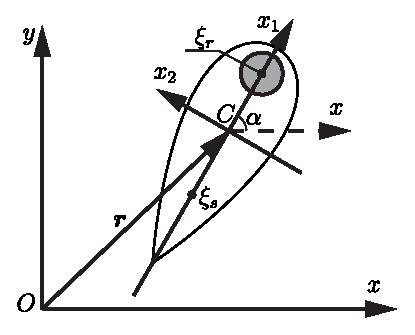
\includegraphics[width=0.9\linewidth]{coords.eps}
		\end{center}
	\end{figure}	
\end{minipage}
\hfill
\begin{minipage}[t]{0.63\linewidth}
	$Oxy$ -- неподвижная система координат,
	
	$Cx_1x_2$ -- подвижная система координат.%, жестко связанная с телом.
	
	$\bs r = (x,\, y)$ радиус-вектор точки $C$, определяющий положение системы.
	
	Угол $\alpha$ определяет ориентацию системы.
	
	Справедливы следующие кинематические соотношения:
	\vspace{-3mm}
	\begin{gather*}	
	%\begin{gathered}
	\dot{x} = v_1 \cos\alpha - v_2 \sin\alpha,\quad \dot{y} = v_1 \sin\alpha + v_2 \cos\alpha, \\
	\dot{\alpha} = \omega.
	%\end{gathered}
	\end{gather*}
	
\end{minipage}	

Описание движения -- уравнения Ньютона-Эйлера в подвижных осях: %, жестко связанных с телом:
\begin{gather*}
\begin{gathered}
m \dot{v}_1 = m v_2 \omega + f_1 (v_1,\, v_2,\, \omega,\, \dot{v}_1,\, \dot{v}_2,\, \dot \omega),\quad m \dot{v}_2 = -m v_1 \omega + f_2 (v_1,\, v_2,\, \omega,\, \dot{v}_1,\, \dot{v}_2,\, \dot \omega),\\
I \dot{\omega} = g (v_1,\, v_2,\, \omega,\, \dot{v}_1,\, \dot{v}_2,\, \dot \omega),
\end{gathered}\label{eq.NE}
\end{gather*}

Для определения вида $ f_1 $, $ f_2 $ и $ g $ воспользуемся уравнениями Кирхгофа, дополнеными слагаемыми, описывающими вязкое сопротивление:% \cite{Borisov_et_al_2016}:
\begin{equation*}
\begin{gathered}
\der{}{t} \pder{T}{v_1} = \omega \pder{T}{v_2} - c_1 v_1 |v_1|,\quad \der{}{t} \pder{T}{v_2} = - \omega \pder{T}{v_1} - c_2 v_2 |v_2|,\\
\der{}{t} \pder{T}{\omega} = v_2 \pder{T}{v_1} - v_1 \pder{T}{v_2} - c_3 \omega |\omega|,
\end{gathered}\label{eq.kirchhoff}
\end{equation*}
%где $T$ --- кинетическая энергия системы (корпус + ротор + жидкость); $c_1$, $c_2$, $c_3$ --- коэффициенты сопротивления.



\end{frame}



%\begin{frame}
%\frametitle{Математическая модель}
%
%	\begin{itemize}
%	
%		%где $m$, $I$ --- масса и момент инерции робота соответственно, $f_1$, $f_2$ --- проекции силы реакции жидкости на подвижные оси, связанные с телом, $g$ --- момент силы реакции жидкости.
%		\item Движение твердого тела в идеальной жидкости при нулевой циркуляции описывается уравнениями Кирхгофа. % их необходимо дополнить слагаемыми, описывающими вязкое трение \cite{Borisov_et_al_2016}:
%		\begin{equation*}
%		\begin{gathered}
%		\der{}{t} \pder{T}{v_1} = \omega \pder{T}{v_2} - c_1 v_1 |v_1|,\quad \der{}{t} \pder{T}{v_2} = - \omega \pder{T}{v_1} - c_2 v_2 |v_2|,\\
%		\der{}{t} \pder{T}{\omega} = v_2 \pder{T}{v_1} - v_1 \pder{T}{v_2} - c_3 \omega |\omega|,
%		\end{gathered}\label{eq.kirchhoff}
%		\end{equation*}
%		где $T$ --- кинетическая энергия системы (корпус + ротор + жидкость), $c_1$, $c_2$, $c_3$ --- коэффициенты сопротивления.
%		
%		Кинетическая энергия системы с точностью до некоторой функции времени имеет вид
%		\begin{gather*}
%		T = \frac{1}{2}(m + \lambda_{11}) v_1^2 + \frac{1}{2}(m + \lambda_{22}) v_2^2 + \frac{1}{2} (I + \lambda_{33}) \omega^2 + \lambda_{23} v_2\omega + \omega k(t),\label{eq.T}\\
%		\begin{gathered}
%		m = m_s + m_r,\quad
%		I = I_s + m_s \xi_s^2 + I_r + m_r \xi_r^2,\quad k(t) = I_r \Omega(t),
%		\end{gathered}\notag
%		\end{gather*}
%	\end{itemize}
%
%\end{frame}


\begin{frame}
\frametitle{Математическая модель. Уравнения движения}

Кинетическая энергия системы с точностью до некоторой функции времени имеет вид:
\begin{gather*}
T = \frac{1}{2}(m + \lambda_{11}) v_1^2 + \frac{1}{2}(m + \lambda_{22}) v_2^2 + \frac{1}{2} (I + \lambda_{33}) \omega^2 + \lambda_{23} v_2\omega + \omega k(t),\label{eq.T}\\
\begin{gathered}
m = m_s + m_r,\quad
I = I_s + m_s \xi_s^2 + I_r + m_r \xi_r^2,\quad k(t) = I_r \Omega(t),
\end{gathered}\notag
\end{gather*}

Полная система уравнений рассматриваемой системы может быть записана в следующей форме:
		\begin{equation*}
		\begin{split}\label{eq.dyn}
		(m + \lambda_{11}) \dot{v}_1 = {} & {} (m + \lambda_{22}) v_2 \omega + \lambda_{23}\omega^2 - c_1 v_1 |v_1|,\\
		(m + \lambda_{22}) \dot{v}_2 + \lambda_{23} \dot{\omega} = {} & {} - (m + \lambda_{11}) v_1 \omega - c_2 v_2 |v_2|,\\
		\lambda_{23,l}\dot{v}_2 + (I + \lambda_{33}) \dot{\omega} = {} & {} (\lambda_{11} - \lambda_{22}) v_1 v_2 - \lambda_{23,r} v_1\omega - c_3 \omega |\omega| - \dot{k}(t),
		\end{split}
		\end{equation*}
		\begin{equation*}
		\dot{x} = v_1 \cos\alpha - v_2 \sin\alpha,\quad \dot{y} = v_1 \sin\alpha + v_2 \cos\alpha,\quad \dot{\alpha} = \omega.
		\end{equation*}

	
	
	 %Сравнивая уравнения \eqref{eq.dyn} с уравнениями Ньютона-Эйлера \eqref{eq.NE}, запишем 
	 Выражения для сил $f_1$, $f_2$ и момента $g$:
	\begin{gather*}
	\begin{gathered}\label{eq.forceTorque}
	f_1 = - \lambda_{11}\dot{v}_1 + \lambda_{22} v_2 \omega + \lambda_{23}\omega^2 - c_1 v_1 |v_1|, \quad
	f_2 = - \lambda_{22} \dot{v}_2 - \lambda_{23} \dot{\omega} - \lambda_{11} v_1 \omega - c_2 v_2 |v_2|,\\
	g = -\lambda_{23}\dot{v}_2 - \lambda_{33} \dot{\omega} + (\lambda_{11} - \lambda_{22}) v_1 v_2 - \lambda_{23} v_1\omega - c_3 \omega |\omega| - \dot{k}(t).
	\end{gathered}
	\end{gather*}
	%где коэффициенты $\lambda_{ij}$ и $c_i$ подлежат определению, а $\dot{k}(t)$ --- определяется управляющим воздействием на ротор.


\end{frame}




%\begin{frame}
%\frametitle{Закон изменения угловой скорости ротора}
%
%	В общем случае, зависимость угловой скорости ротора от времени будет иметь характерные переходные интервалы, соответствующие разгону и торможению 
%	
%		\scriptsize 
%		\vspace{-4mm}
%		\begin{equation*}
%		\omega_r(t) =
%		\begin{cases}
%		
%		\omega_1 & t \in \left[ nT;  nT + t_1 \right] ,\\
%		
%		\frac{(\omega_2 - \omega_1)(t-nT)}{t_2} - \frac{(\omega_2 - \omega_1)(t_1+t_2)}{t_2} + \omega_2 & t \in \left[ nT + t_1;  nT + t_1+t_2 \right], \\
%		
%		\omega_2 & t \in \left[ nT + t_1+t_2;  nT + t_1+t_2+t_3 \right] ,\\
%		
%		\frac{(\omega_1 - \omega_2)(t-nT)}{t_4} - \frac{(\omega_1 - \omega_2)(t_1+t_2+t_3+t_4)}{t_4} + \omega_1 &t \in \left[ nT + t_1 + t_2+t_3;  nT + t_1+t_2+t_3+t_4 \right] ,
%		
%		\end{cases}
%		\label{omegaRotorGeneral}
%		\end{equation*}
%		
%		\small
%		где $n \in \mathbf{N}$, $T$ -- период управляющего воздействия; $ \omega_1, \omega_2 $ -- амплитуды угловой скорости вращения ротора по часовой стрелке и против часовой стрелки соответственно; $t_1, t_2, t_3, t_4$ -- задают продолжительность по времени характерных интервалов угловой скорости вращения ротора. 
%		
%			%\framebreak
%		
%		%Графически данная зависимость приведена на рисунке
%		
%		\begin{minipage}[t]{0.47\linewidth}
%			\begin{figure}[!ht]
%				\centering
%				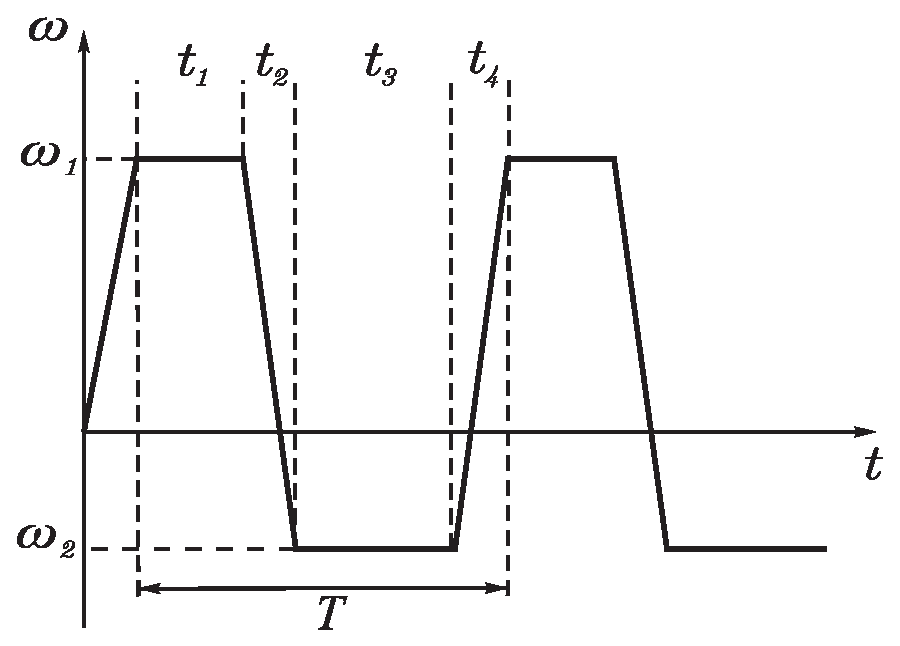
\includegraphics[height=33mm]{ControlAction.eps}
%			\end{figure}
%			
%		\end{minipage}	
%		\hfill
%		\begin{minipage}[t]{0.47\linewidth}
%			\begin{figure}[!ht]
%				\centering
%				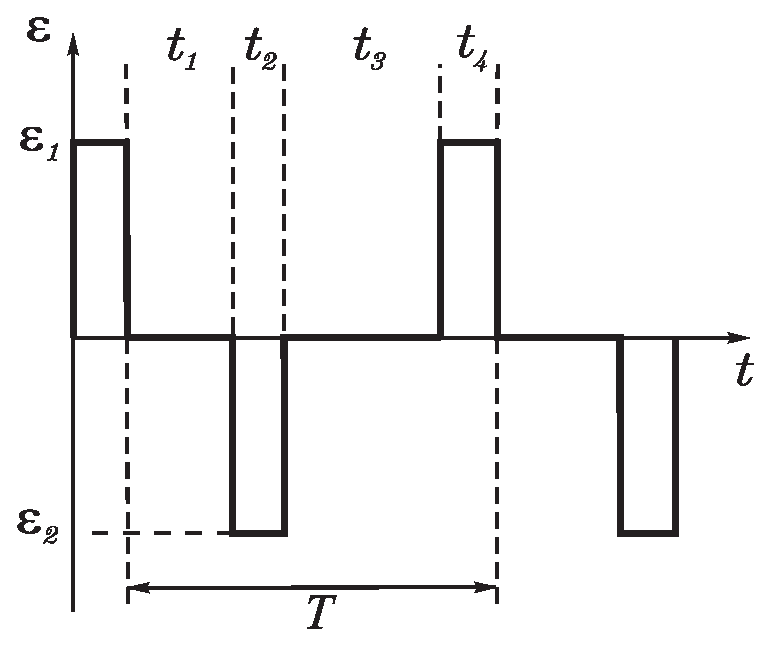
\includegraphics[height=33mm]{ControlActionEpsilon.eps}
%			\end{figure}
%		\end{minipage}	
%%		\begin{figure}[!ht]
%%			\centering
%%			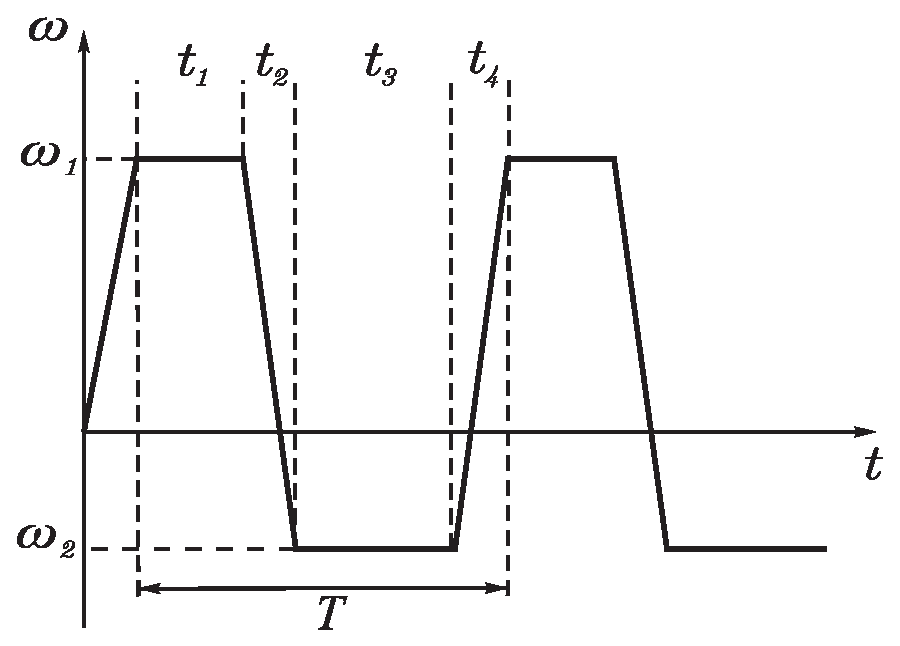
\includegraphics[width=0.4\linewidth]{ControlAction.eps}
%%		\end{figure}
%	
%	
%\end{frame}
%
%\begin{frame}
%\frametitle{Методика проведения экспериментов}
%
%	\begin{itemize}
%		\item Эксперименты проводились в бассейне размерами $2 \times 1.2$ метра. 
%		\item Траектория движения робота и его ориентация в процессе движения восстанавливались с помощью системы захвата движения фирмы Vicon, включающей 7 камер, расположенных по периметру бассейна. 
%		\item Типовая траектория движения, восстановленная с помощью системы захвата движения и наложенная на кадр с видеозаписи в бассейне
%		
%		\begin{figure}[!h]
%			\centering
%			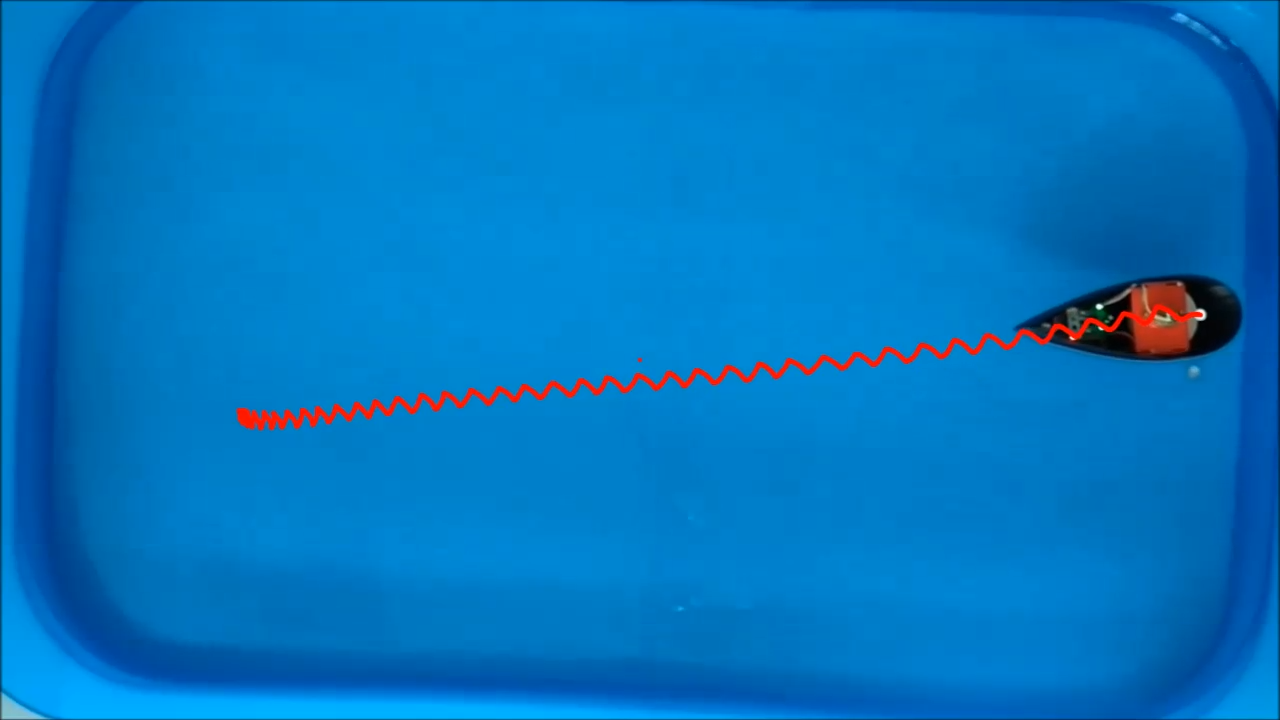
\includegraphics[width=0.8\linewidth]{Frame1col.png}
%		\end{figure}
%	\end{itemize}
%
%
%
%\end{frame}

\begin{frame}
\frametitle{Закон изменения угловой скорости ротора}

Аналитическая запись функции угловой скорости ротора

\scriptsize 
\begin{equation*}
\omega_r(t) =
\begin{cases}

\omega_1 & t \in \left[ nT;  nT + t_1 \right] ,\\

\frac{(\omega_2 - \omega_1)(t-nT)}{t_2} - \frac{(\omega_2 - \omega_1)(t_1+t_2)}{t_2} + \omega_2 & t \in \left[ nT + t_1;  nT + t_1+t_2 \right], \\

\omega_2 & t \in \left[ nT + t_1+t_2;  nT + t_1+t_2+t_3 \right] ,\\

\frac{(\omega_1 - \omega_2)(t-nT)}{t_4} - \frac{(\omega_1 - \omega_2)(t_1+t_2+t_3+t_4)}{t_4} + \omega_1 &t \in \left[ nT + t_1 + t_2+t_3;  nT + t_1+t_2+t_3+t_4 \right] ,

\end{cases}
\label{omegaRotorGeneral}
\end{equation*}

\small 

\begin{minipage}[t]{0.47\linewidth}
График угловой скорости ротора

	\begin{figure}[!ht]
		\centering
		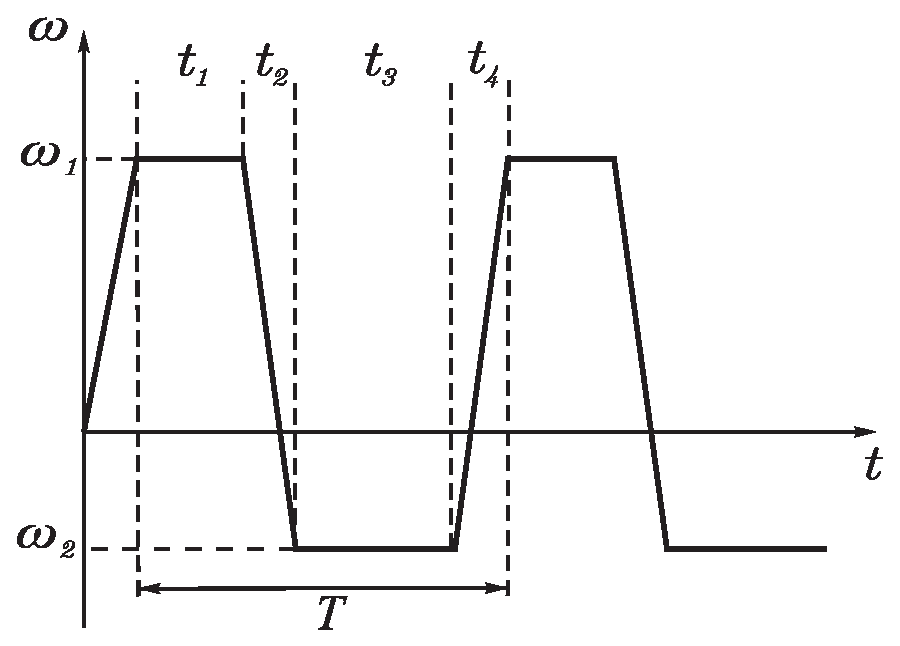
\includegraphics[height=30 mm]{ControlAction.eps}
	\end{figure}
	
\end{minipage}	
\hfill
\begin{minipage}[t]{0.47\linewidth}
%	\begin{figure}[!ht]
%		\centering
%		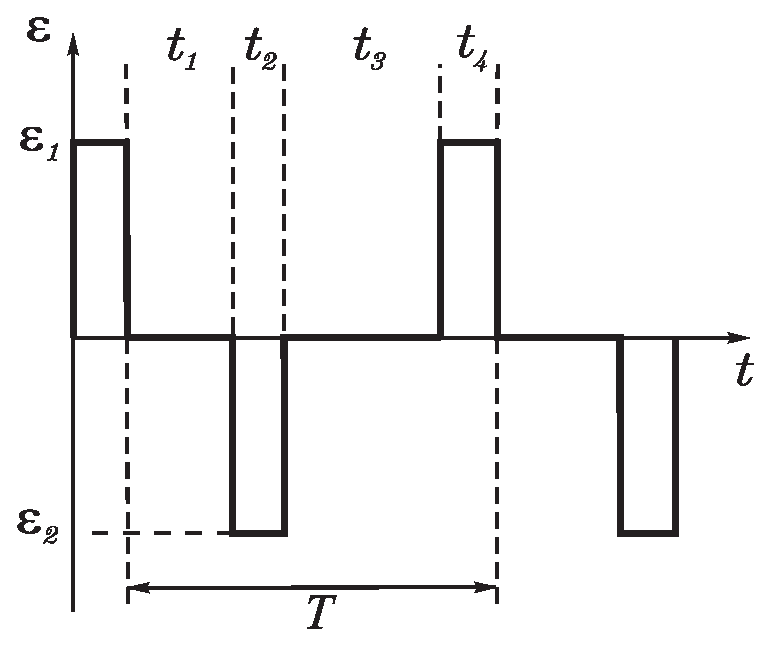
\includegraphics[height=30 mm]{ControlActionEpsilon.eps}
%	\end{figure}
Кадр эксперимента с наложенной траекторией движения.

\begin{figure}[!h]
	\centering
	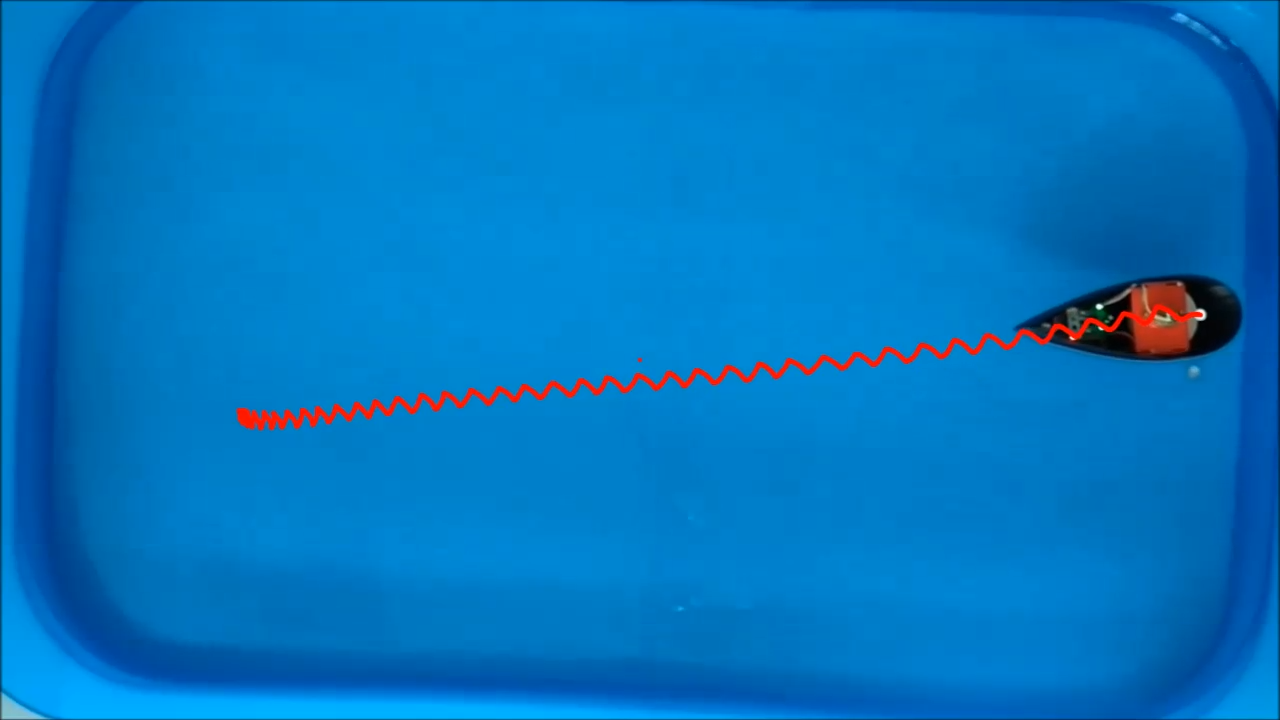
\includegraphics[width=1\linewidth]{Frame1col.png}
\end{figure}

\end{minipage}	
%		\begin{figure}[!ht]
%			\centering
%			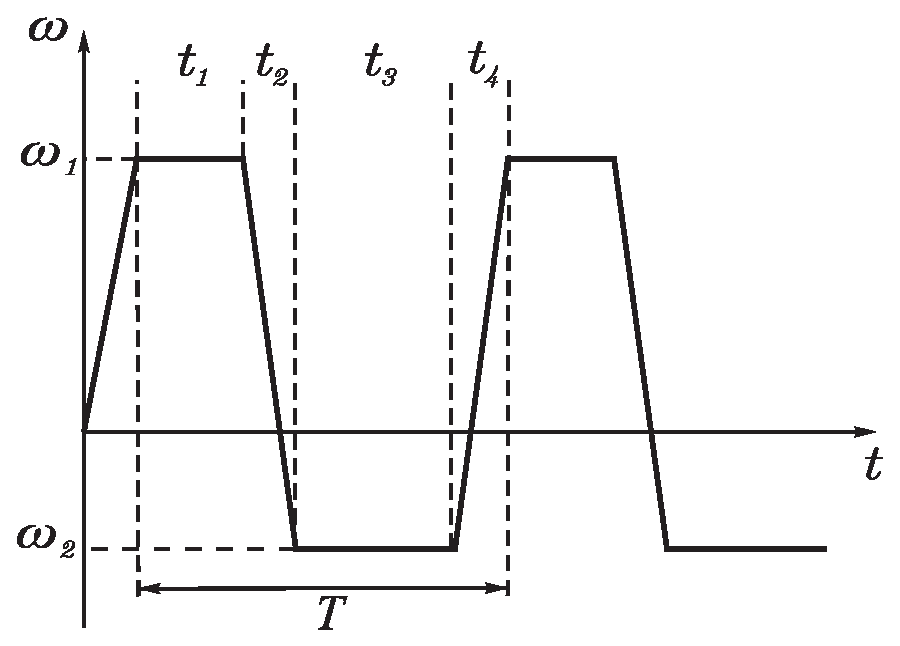
\includegraphics[width=0.4\linewidth]{ControlAction.eps}
%		\end{figure}


\vspace{5mm}



\end{frame}

\begin{frame}
\frametitle{Движение вдоль прямой}

1. $t_1=t_3$, $ t_2 = t_4$; \quad $ \omega_1 = \omega_{max} $, $ \omega_2 = -\omega_{max} $.

\begin{minipage}[t]{0.3\linewidth}
	\begin{figure}[!ht]
		\centering
		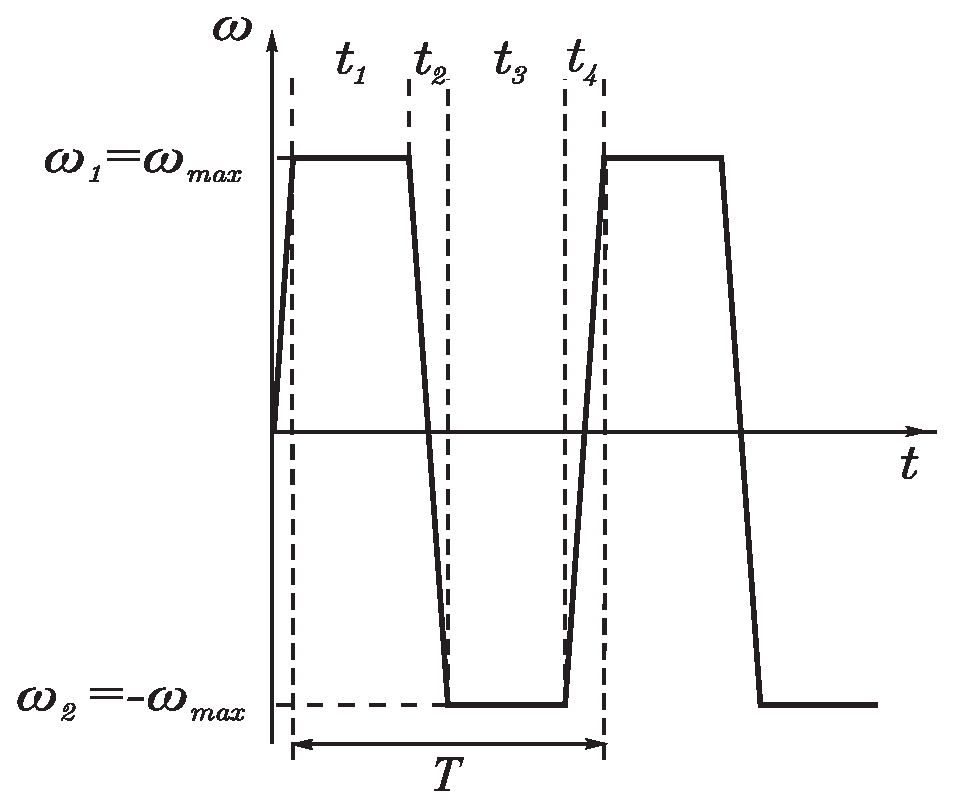
\includegraphics[width=1\linewidth]{ControlActionLine.eps}
	\end{figure}	
\end{minipage}
\hfill
\begin{minipage}[t]{0.68\linewidth}
	\begin{figure}[!ht]
		\centering
		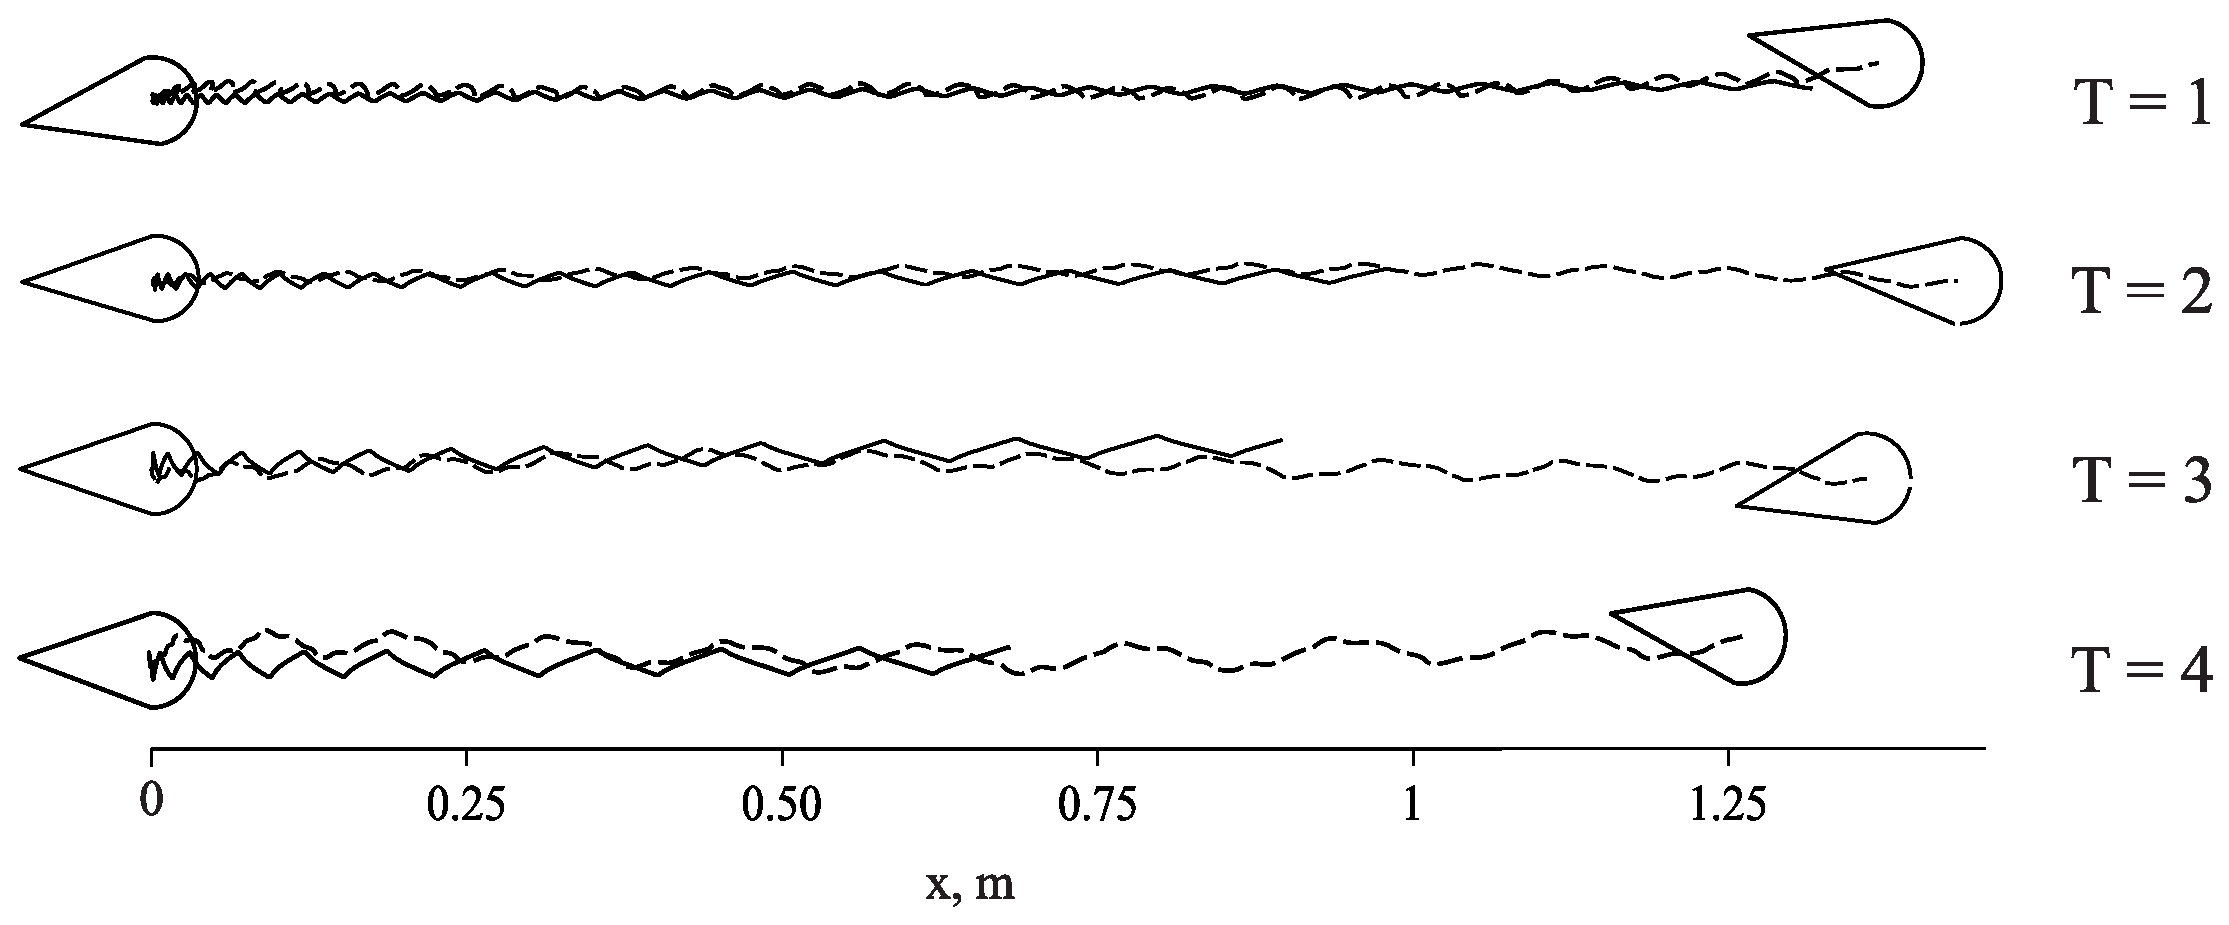
\includegraphics[width=1\linewidth]{AllTrajectories_new.eps}
	\end{figure}
\end{minipage}	
	
2. 	$t_1=t_3$, $ t_2 = t_4$, $ T=2 $ с.; \quad $ \omega_1 - \omega_2 = const$

\begin{minipage}[h]{0.47\linewidth}
	\center{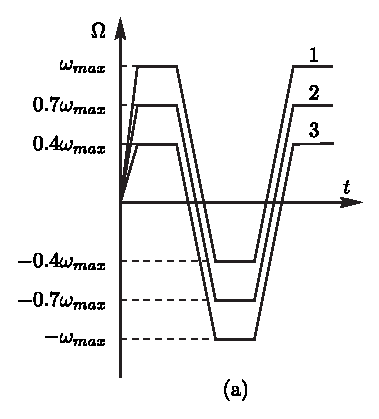
\includegraphics[width=0.6\linewidth]{ControlActionPlots3.eps} }
\end{minipage}
\hfill
\begin{minipage}[h]{0.47\linewidth}
	\center{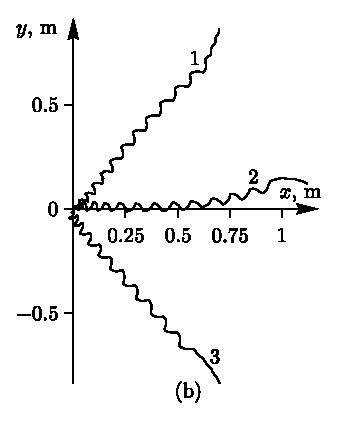
\includegraphics[width=0.6\linewidth]{Plots3.eps}}
\end{minipage}


\end{frame}



\begin{frame}
\frametitle{Движение вдоль окружности}

1. $t_1 \neq t_3$, $t_2 = t_4$ с; \quad	$ \omega_1 = \omega_{max} $, $ \omega_2 = -\omega_{max} $; \quad $ k_1 = t_3 / t_1 $
		
	
	\begin{minipage}[t]{0.47\linewidth}
	{Угловая скорость ротора}
			\center{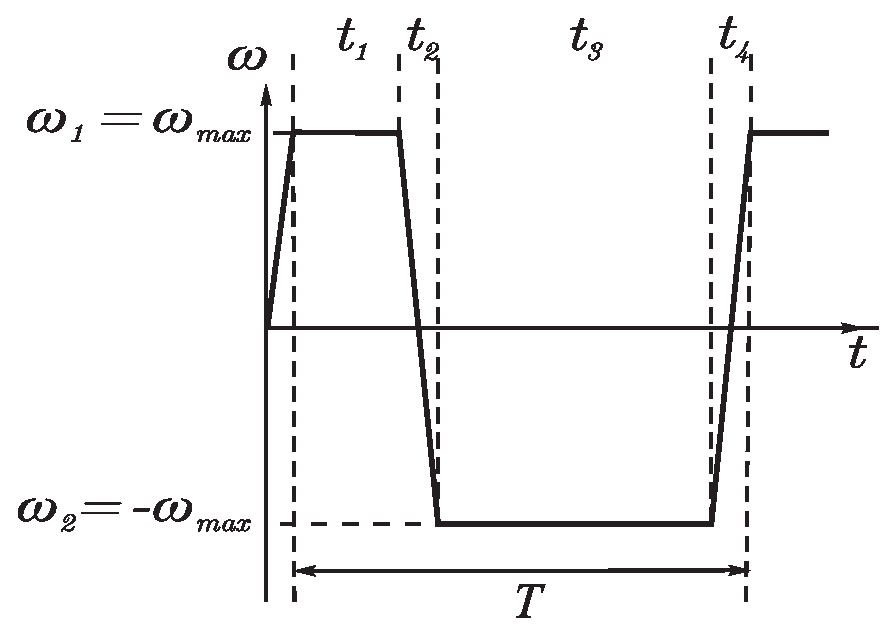
\includegraphics[width=0.7\linewidth]{ControlActionCircle.eps}}
	\end{minipage}
	\hfill
	\begin{minipage}[t]{0.47\linewidth}
		{Траектория движения робота}
		\center{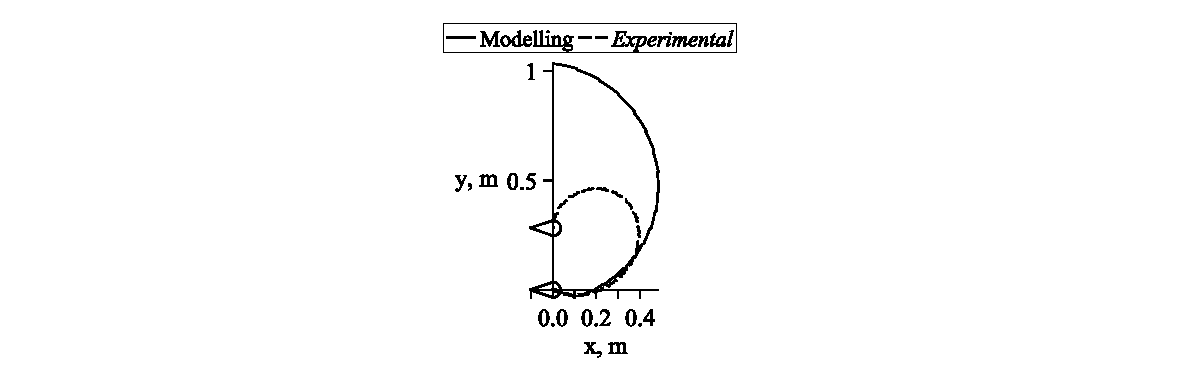
\includegraphics[width=0.35\linewidth]{xyCircleWmax.eps}}
	\end{minipage}

\vspace{4mm}

2. $t_1 = t_3$, $t_2 \neq t_4$ с; \quad $ \omega_1 = \omega_{max} $, $ \omega_2 = -\omega_{max} $ \quad $ k_2 = t_2 / t_4 $

\begin{minipage}[t]{0.47\linewidth}
	{Угловая скорость ротора}
	\center{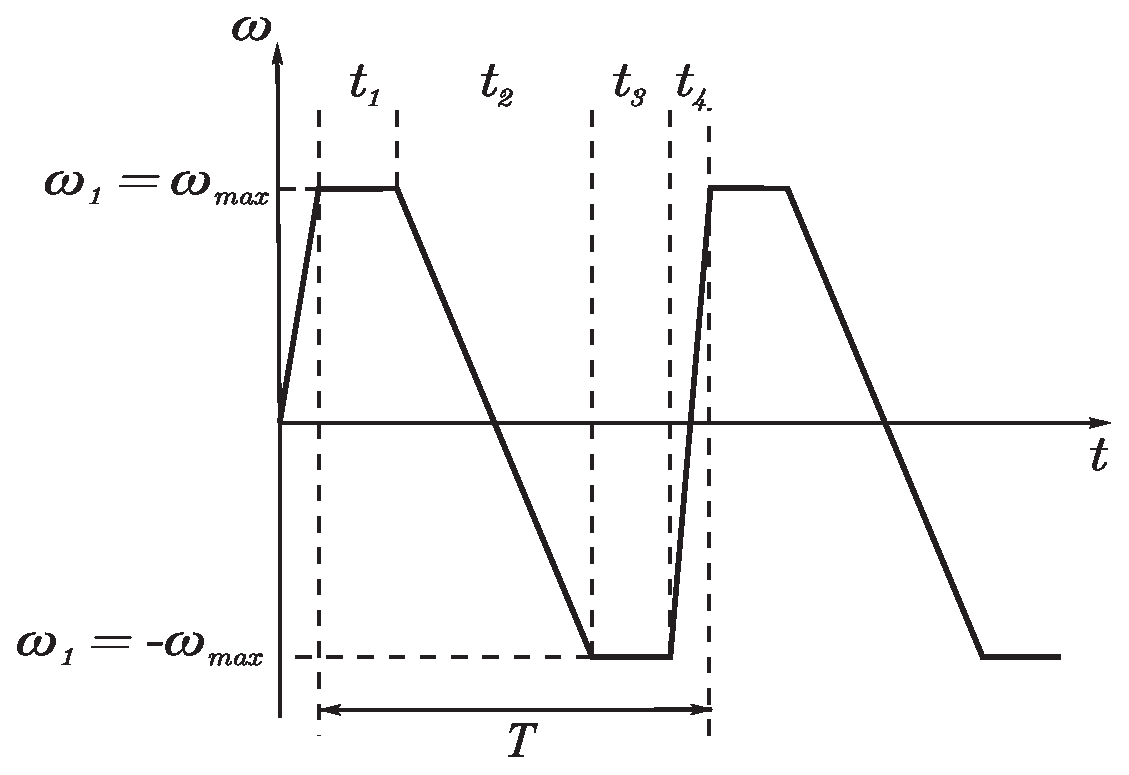
\includegraphics[width=0.7\linewidth]{ControlActionOur1.eps}}
\end{minipage}
\hfill
\begin{minipage}[t]{0.47\linewidth}
	{Траектория движения робота}
	\center{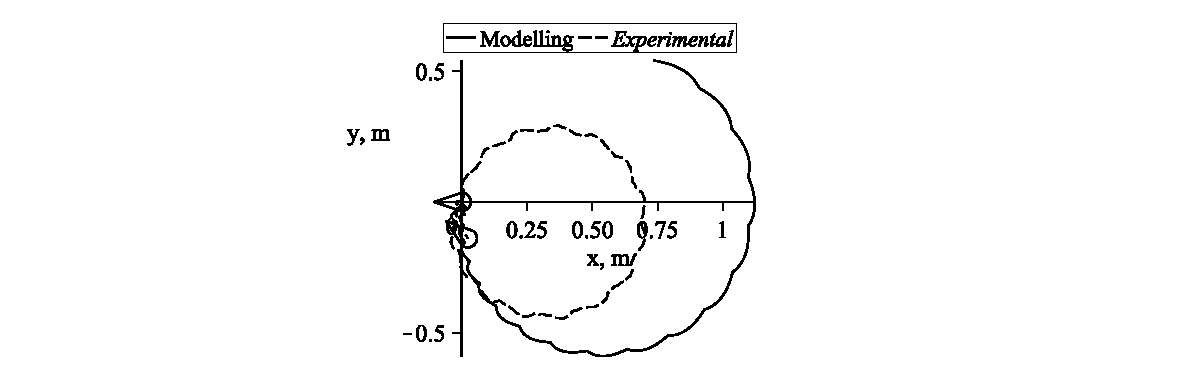
\includegraphics[width=0.5\linewidth]{xyCircleOur.eps}}
\end{minipage}

\end{frame}


\begin{frame}
\frametitle{Движение вдоль окружности}

Зависимость радиуса траектории движения робота от $k_1 ={t_3}/{t_1}$ построенная по экспериментам при $k_1 = 2, 3, 5, 10$

\begin{figure}[!ht]
	\centering
	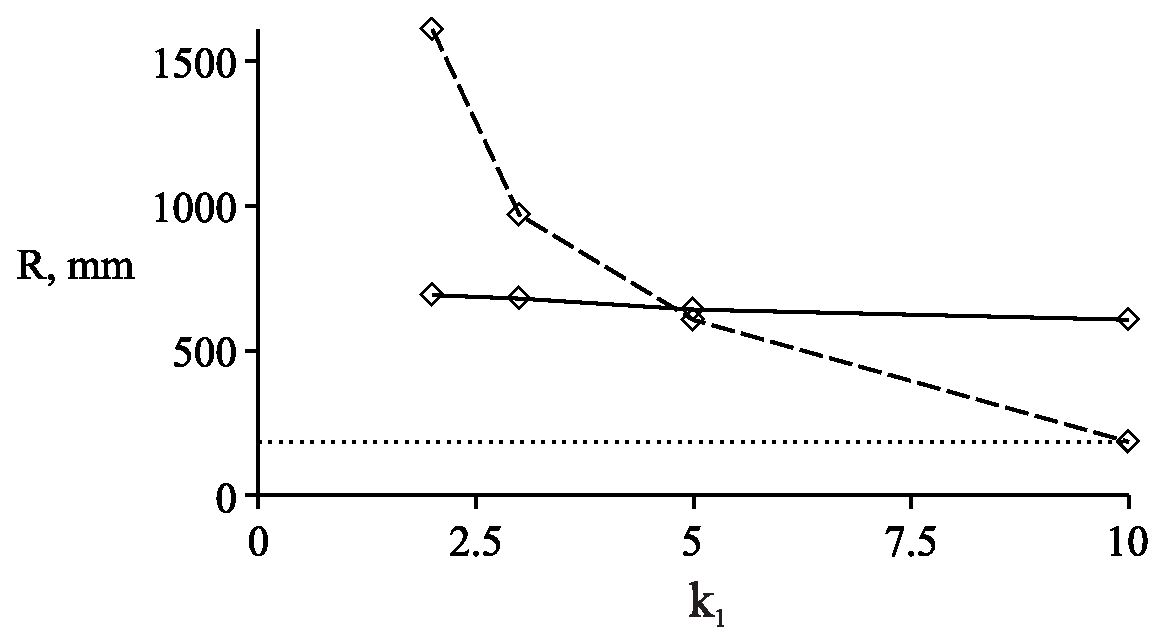
\includegraphics[width=0.5\linewidth]{kRDependence+Theor_T=3,W=max.eps}
\end{figure}
	
Зависимость радиуса траектории движения робота от $k_2 = {t_2}/{t_4}$ построенная по экспериментам при $k_2 = 10, 20, 30, 40$

\begin{figure}[!ht]
	\centering
	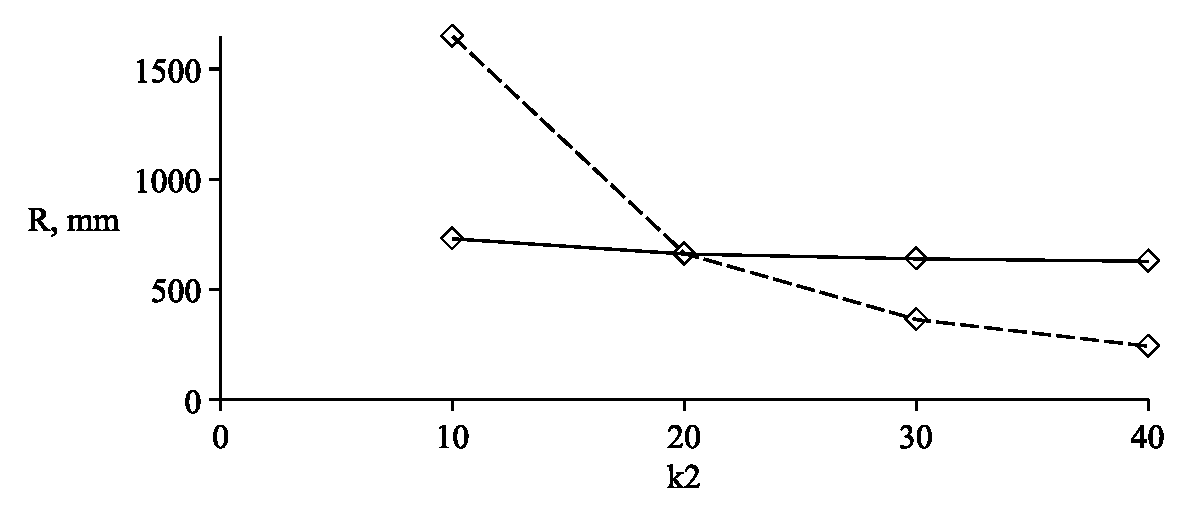
\includegraphics[width=0.5\linewidth]{nROur.eps}
\end{figure}		
%\begin{minipage}[t]{0.47\linewidth}
%	{Зависимость радиуса траектории движения робота от $k_1 = \frac{t_3}{t_1}$ при эксперименте (штриховая линия) и моделировании (сплошная линия) построенная по экспериментам при $k_1 = 2, 3, 5, 10$}
%	\center{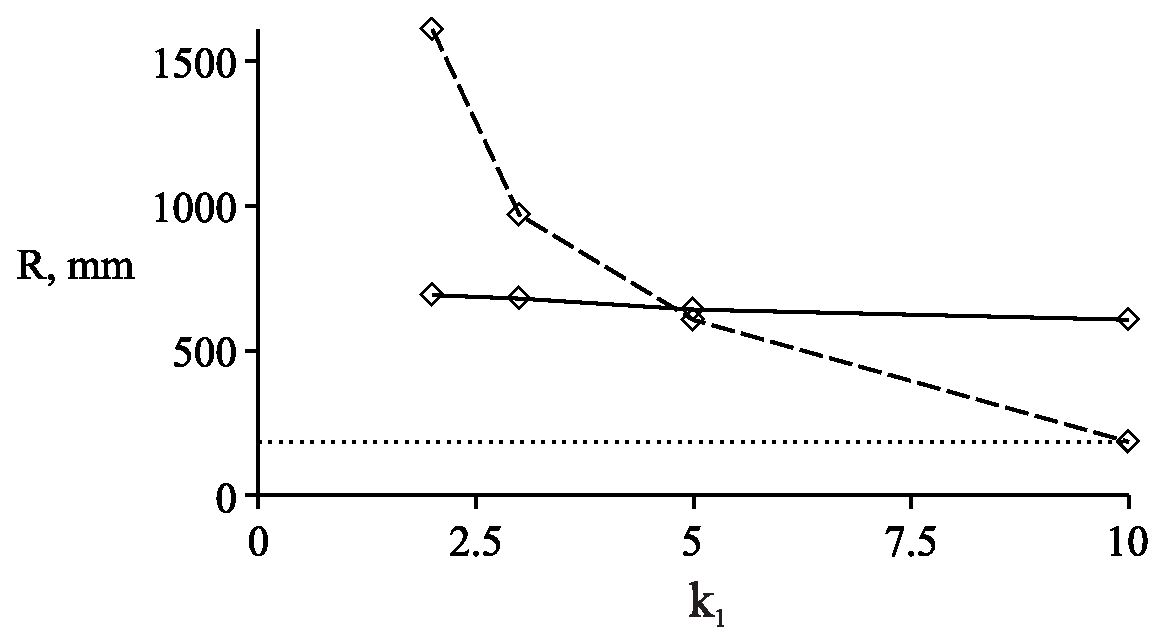
\includegraphics[width=0.9\linewidth]{kRDependence+Theor_T=3,W=max.eps}}
%\end{minipage}
%\hfill
%\begin{minipage}[t]{0.47\linewidth}
%	{Зависимость радиуса траектории движения робота от $k_2 = \frac{t_2}{t_4}$ при эксперименте (штриховая линия) и моделировании (сплошная линия) построенная по экспериментам при $k_2 = 10, 20, 30, 40$}
%	\center{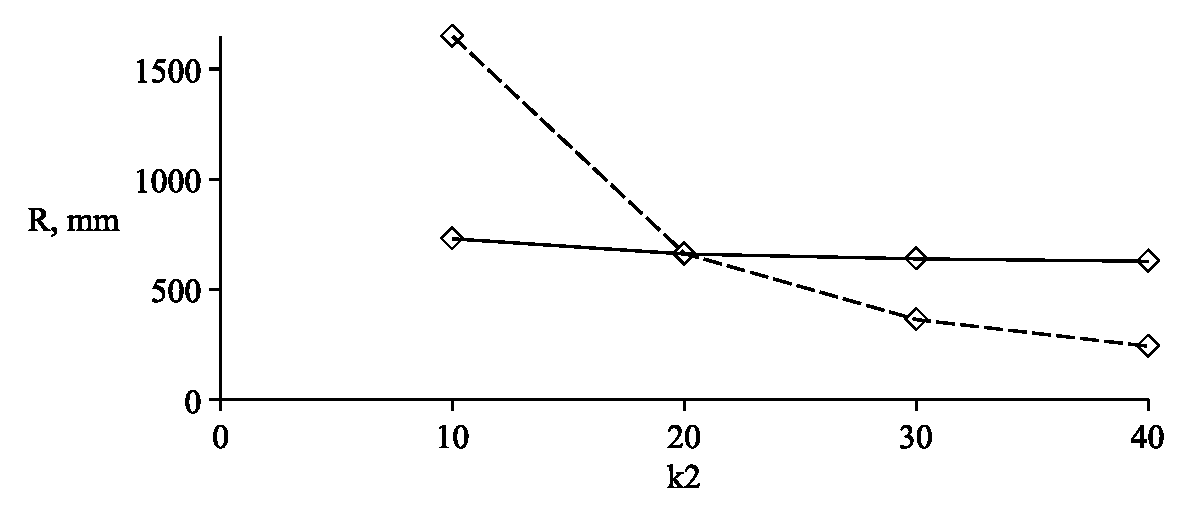
\includegraphics[width=1.05\linewidth]{nROur.eps}}
%\end{minipage}

\end{frame}


%\begin{frame}
%\frametitle{Выводы}
%\begin{itemize}
%	\item Рассматриваемая теоретическая модель управляемого движения водного робота качественно правильно описывает его движение. Cимметричное управляющее воздействие -- движение вдоль прямой. Асимметричное управляющее воздействие -- движение вдоль окружности.
%	
%	\item Сдвиг управляющего воздействия $\omega(t) \rightarrow \omega_0 + \omega(t)$ не влияет на форму траектории. На размер и форму траектории движения влияет асимметрия управляющего воздействия на его периоде.
%	
%	\item Количественного согласования результатов моделирования и экспериментов можно достичь для конкретных тестов, проводя перерасчет коэффициентов под конкретные экспериментальные данные.
%	
%	\item Комбинируя описанные маневры, можно двигаться по сложной траектории.
%	
%	%\item Рассматриваемая теоретическая модель управляемого движения водного робота качественно правильно  описывает его движение вдоль окружности, которое реализуется асимметричным на периоде управляющим воздействием.
%	%\item На размер и форму траектории движения влияет асимметрия управляющего воздействия на его периоде. Изменение направления движения -- поворот, может быть реализован либо при изменении продолжительности интервала вращения с постоянной угловой скоростью, либо вращением ротора по и против часовой стрелки с различными угловыми ускорениями.
%	%\item Количественного согласования результатов моделирования и экспериментов, как и в при движении вдоль прямой, можно достичь для конкретных тестов, проводя перерасчет коэффициентов под конкретные экспериментальные данные, полученные при движении вдоль окружности.
%\end{itemize}
%
%\end{frame}
%
%
%\begin{frame}
%\frametitle{Экспериментальные исследования. Движение вдоль сложных траекторий}
%
%
%	{Управление для слалома}
%	\centering
%	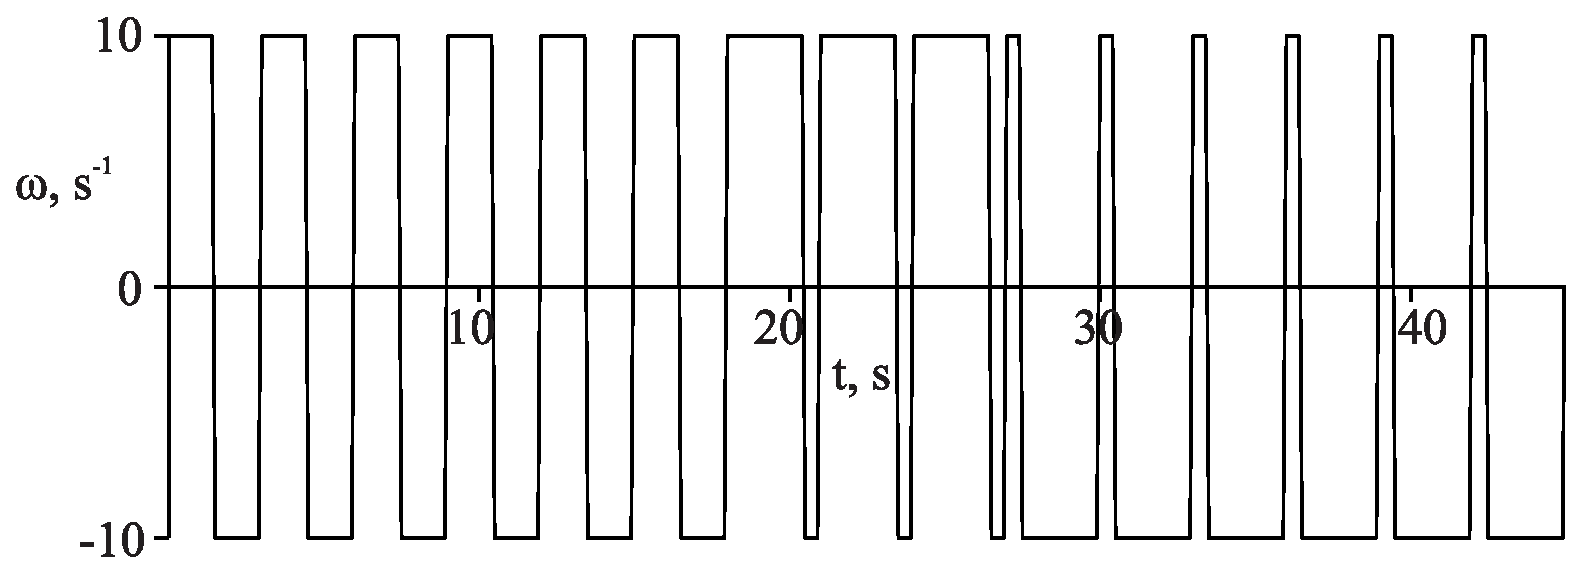
\includegraphics[width=0.7\linewidth]{ControlActionComplexTr.eps}
%
%	{Траектория движения робота при эксперименте (штриховая линия) и моделировании (сплошная линия)}
%	\centering
%	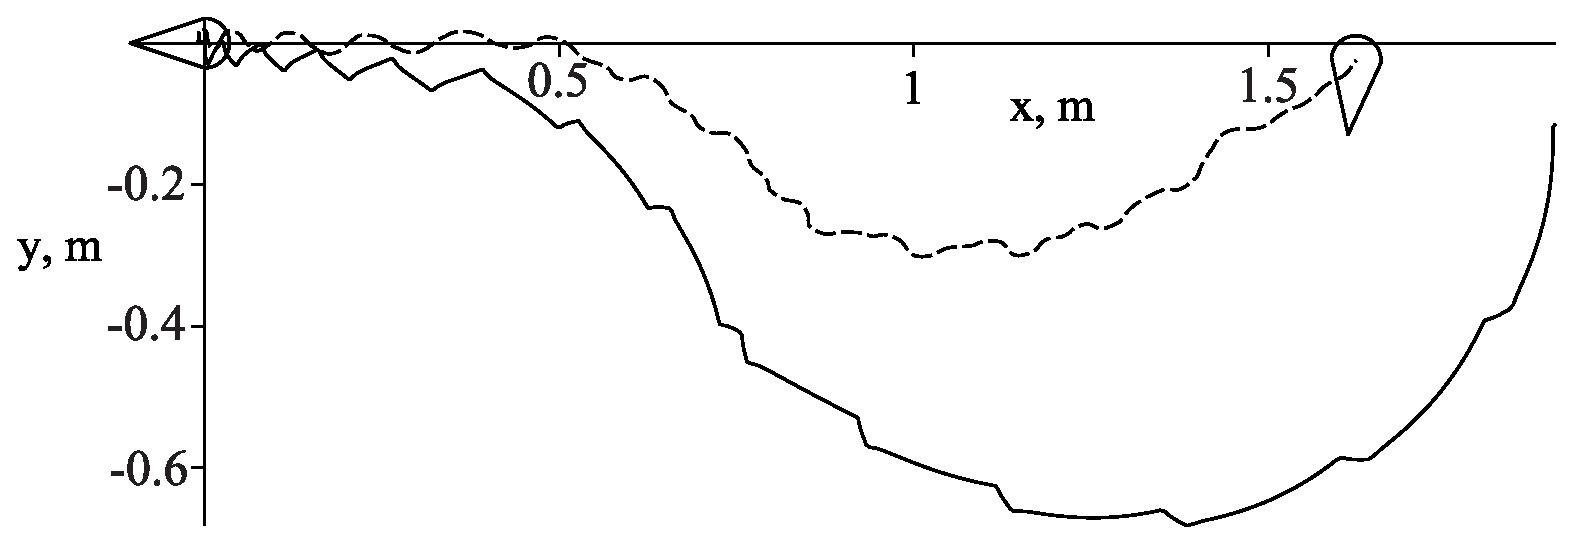
\includegraphics[width=0.7\linewidth]{ComplexTr.eps}
%
%
%\end{frame}

%\begin{frame}
%\frametitle{Экспериментальные исследования. Видео.}
%
%\begin{figure}[ht]
%%	%\vspace{-7pt}
%%	%\hspace*{-28.5pt}
%	\includemovie[
%%	%autoplay,
%%	%repeat,
%%	%poster=ComplexTr1.png,
%	inline=false,
%	text={Video}
%	]{\textwidth}{0.6\textwidth}{Video.mp4}
%\end{figure}

%\movie[width=1\textwidth]{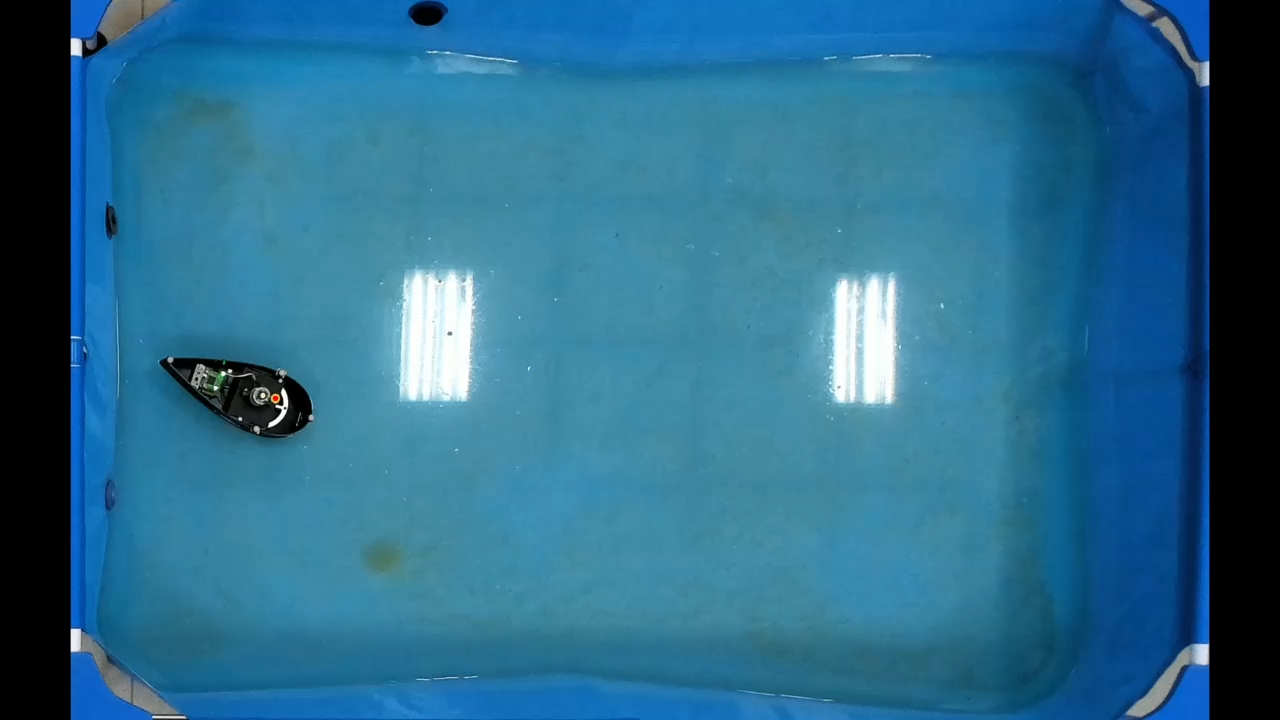
\includegraphics[width=1\textwidth]{ComplexTr1.png}}{Video.mp4}
%\includemedia[activate=onclick, width=0.5\textwidth]{\includegraphics{ComplexTr1.png}}{123.mp4}
%\includemedia[
%activate=pageopen,
%width=1280pt,height=720pt,
%addresource=123.mp4,
%flashvars={
%	source=123.mp4}
%]{}{VPlayer.swf}

%\includemedia[
%width=\textwidth,%height=6cm,
%%width=1\linewidth,
%activate=onclick, %deactivate=onclick,
%%playbutton=fancy,
%passcontext,
%transparent,
%addresource=Video.flv,
%flashvars={source=Video.flv}
%]{click}{VPlayer.swf}

%\includemedia[activate=pageopen, width=0.5\textwidth]
%{video}{Video.swf}
%
%\end{frame}

\begin{frame}
\frametitle{Движение вдоль сложных траекторий. Выводы}

Пример движения вдоль сложной траектории

{
	\centering
	\includegraphics[width=0.45\linewidth]{ControlActionComplexTr.eps} \hspace{5mm}
	\includegraphics[width=0.45\linewidth]{ComplexTr.eps}
}
\textbf{Выводы по экспериментам с недеформируемым водным роботом с острой кромкой}
\begin{itemize}
	\item Рассматриваемая теоретическая модель управляемого движения водного робота качественно правильно описывает его движение. Cимметричное управляющее воздействие -- движение вдоль прямой. Асимметричное управляющее воздействие -- движение вдоль окружности.
	
	\item Сдвиг управляющего воздействия $\omega(t) \rightarrow \omega_0 + \omega(t)$ не влияет на форму траектории. На размер и форму траектории движения влияет асимметрия управляющего воздействия на его периоде.
	
	\item Комбинируя описанные маневры, можно двигаться по сложной траектории.
	
	\item Количественное отклонение может быть минимизировано уточнением коэффициентов модели движения для различных движений.
	
\end{itemize}

\end{frame}

\begin{frame}
\frametitle{Заключение}


\textbf{Выводы по работе}

\begin{itemize}
	\item Разработаны математические модели движения, конструкции, алгоритмы управления для роботов, перемещающихся в жидкости за счет вращения внутренних роторов: безвинтового подводного робота в форме эллипсоида и недеформируемого водного робота с острой кромкой. Проведены экспериментальные исследования.
	\item Экспериментально показано, что движение за счет вращения внутренних роторов возможно.
	\item Модели, построенные в рамках теории идеальной жидкости качественно адекватно описывают движение водных роботов, перемещающихся за счет вращения внутренних роторов. Адекватность математических моделей подтверждена экспериментально. 
	\item Для увеличения количественного согласования необходимо учитывать вязкое сопротивление, возникновение вихревых структур, с большой точностью определять коэффициенты присоединенных масс.
\end{itemize}

\end{frame}

\begin{frame}[shrink=25]
\frametitle{Конференции, публикации}

\textbf{Конференции:} 

\begin{itemize}
	
\item Молодые ученые -- ускорению научно-технического прогресса в XXI веке 2016 (Ижевск),

\item GDIS-2016 (Ижевск), 

\item МИКМУС-2018 (Москва), 

\item Scientific Heritage of Sergey A. Chaplygin: nonholonomic mechanics, vortex structures and hydrodynamics 2019 (Чебоксары), 

\item Экстремальная робототехника-2019  (Санкт-Петербург), 

\item CLAWAR-2020~(Москва).

\end{itemize}

\textbf{Публикации:}
\begin{itemize}

\item Ветчанин Е. В, Караваев Ю.Л., Калинкин А.А., Пивоварова Е.Н., Клековкин А.В. Модель безвинтового подводного робота. Вестник Удмуртского университета. Математика. Механика. Компьютерные науки. 2015. Т.25. №.4. С. 544-553. (ВАК)

\item Y. Karavaev, A. Kilin, A. Klekovkin. Experimental investigations of the controlled motion of a screwless underwater robot // Regular and Chaotic Dynamics. 2016. Т.21. №. 7-8. С. 918-926 (WoS)

%\item Klekovkin A.V., Karavaev Yu.L., Kilin A.A., Mamaev I.S. Control screwless fish-like robot with internal rotor // Extreme Robotics,  2019, Vol.1, no. 1, pp. 220-225 (РИНЦ)

\item Y. Karavaev, A. Klekovkin, I. Mamaev, V. Tenenev, E. Vetchanin, "A Simple Physical Model for Control of an Propellerless Aquatic Robot",  Journal of Mechanisms and Robotics, 2020. Направлена в журнал. (WoS)


\end{itemize}

\textbf{Патенты:}
\begin{itemize}
	%	\item № 2015615728. Программа для управления безвинтовым надводным роботом // А.В. Борисов, И.С. Мамаев, А.А. Килин, Ю.Л. Караваев, А.В. Клековкин, А.В. Шелухо, А.И. Кленов, Е.В. Ветчанин, В.А. Тененев. Заявитель и патентообладатель – ФБГОУ ВО «ИжГТУ имени М.Т. Калашникова»; Заявка: 2015612643, 07.04.2015, опубл. 22.05.2015
		
	\item Патент на полезную модель. №172254 РФ. Безвинтовой подводный робот //  А.В. Борисов, И.С. Мамаев, А.А. Килин, А.А. Калинкин, Ю.Л. Караваев, А.В. Клековкин, Е.В. Ветчанин; %заявитель и патентообладатель – ФБГОУ ВО «ИжГТУ имени М.Т. Калашникова»; Заявка: 2016144812, 15.11.2016, опубл. 
	3.07.2017
		
	\item № 2017613219. Программа для управления безвинтовым подводным роботом // А.В. Борисов, И.С. Мамаев, А.А. Килин, Ю.Л. Караваев, А.В. Клековкин. %Заявитель и патентообладатель – ФБГОУ ВО «ИжГТУ имени М.Т. Калашникова»; Заявка: 2016662663, 22.11.2016, опубл. 
	16.03.2017
		
	\item № 2019612284. Программа управления безвинтовым надводным роботом с внутренним ротором // А.В. Борисов, И.С. Мамаев, А.А. Килин, А.В. Клековкин, Ю.Л. Караваев. %Заявитель и патентообладатель – ФБГОУ ВО "ИжГТУ имени М.Т. Калашникова"; Заявка: 2019610925, 04.02.2019, опубл. 
	14.02.2019
\end{itemize}

\end{frame}

%%%%%%%%%%%%%%%%%%%%%%%%%%%%%%%%%%%%%%%%%%%%%%%%%%%%%%%%%%%%%%%%%%%%%%%%%%%%%%%%%%%%%%%%%%%%
       % Настройки заглавной странице
%\begin{frame}
%    \frametitle{Научная новизна}
%    \begin{itemize}
%        \item Впервые реализован \dots
%        \item Разработана программа \dots
%        \item Впервые проведён анализ \dots
%        \item Предложена схема \dots
%    \end{itemize}
%\end{frame}
%\note{
%    Проговаривается вслух научная новизна
%}
%
%\begin{frame}
%    \frametitle{Научная и практическая значимость}
%    \begin{itemize}
%        \item Получены выражения для \dots.
%        \item Определены условия \dots.
%        \item Разработаны устройства \dots.
%    \end{itemize}
%\end{frame}
%\note{
%    Проговариваются вслух научная и практическая значимость
%}
%
%\begin{frame}
%    \frametitle{Свидетельство о регистрации программы}
%    \begin{figure}[h]
%        \centering
%        \includegraphics[height=0.7\textheight]{registration}
%    \end{figure}
%\end{frame}
%\note{
%    Получено свидетельство о регистрации разработанной программы \textsc{Hello~world™}.
%}
%
%\begin{frame}
%    \frametitle{Акт о внедрении}
%    \begin{figure}[h]
%        \centering
%        \fbox{
%            \begin{minipage}[t]{0.4\linewidth}
%                \includegraphics[width=\linewidth]{implementation}
%            \end{minipage}
%        }
%    \end{figure}
%\end{frame}
%\note{
%    Получен акт о внедрении.
%}

% \begin{frame} % публикации на одной странице
%\begin{frame}[t,allowframebreaks] % публикации на нескольких страницах
%    \frametitle{Основные публикации}
%    \nocite{vakbib1}%
%    \nocite{vakbib2}%
%    %
%    %% authorwos
%    \nocite{wosbib1}%
%    %
%    %% authorscopus
%    \nocite{scbib1}%
%    %
%    %% authorconf
%    \nocite{confbib1}%
%    \nocite{confbib2}%
%    %
%    %% authorother
%    \nocite{bib1}%
%    \nocite{bib2}%
%    \ifnumequal{\value{bibliosel}}{0}{
%        \insertbiblioauthor
%    }{
%        \printbibliography%
%    }
%\end{frame}
%\note{
%    Результаты работы опубликованы в N печатных изданиях, в т.ч. M реферируемых изданиях.
%}




    % Последние слайды презентации
\appendix
%\begin{frame}
%    \frametitle{Ответы на замечания ведущей организации НИИ~<<Рога~и~копыта>>}
%    \begin{itemize}
%        \item Замечание -- ответ
%        \item Замечание -- ответ
%        \item Замечание -- ответ
%        \item Замечание -- ответ
%        \item Замечание -- ответ
%    \end{itemize}
%\end{frame}
%
%\begin{frame}
%    \frametitle{Ответы на замечания оф. оппонента Иванова\,И.\,И}
%    \begin{itemize}
%        \item Замечание -- ответ
%        \item Замечание -- ответ
%        \item Замечание -- ответ
%        \item Замечание -- ответ
%        \item Замечание -- ответ
%    \end{itemize}
%\end{frame}
%
%\begin{frame}
%    \frametitle{Ответы на замечания Петрова\,П.\,П}
%    \begin{itemize}
%        \item Замечание -- ответ
%        \item Замечание -- ответ
%        \item Замечание -- ответ
%        \item Замечание -- ответ
%        \item Замечание -- ответ
%    \end{itemize}
%\end{frame}

%\begin{frame}
%\frametitle{Участие в конференциях}
%\begin{itemize}
%	\item IV Всероссийская научно-техническая конференция аспирантов, магистрантов и молодых ученых с международным участием «Молодые ученые -- ускорению научно-технического прогресса в XXI веке». (Ижевск, 2016).
%	\item Шестая международная конференция «Geometry, Dynamics, Integrable Systems -- GDIS 2016» (Ижевск, 2016 г.)
%	\item Машиноведение и инновации. Конференция молодых учёных и студентов (МИКМУС-2018) (Москва, 2018 г.)
%	\item International Conference "Scientific Heritage of Sergey A. Chaplygin: nonholonomic mechanics, vortex structures and hydrodynamics" (Чебоксары, 2019 г.)
%	\item 30-я международная научно-техническая конференция "Экстремальная робототехника-2019" (Санкт-Петербург, 2019 г.)	
%	\item 23rd issue of the International Conference Series on Climbing and Walking Robots and the Support Technologies for Mobile Machines –- CLAWAR 2020 (Москва, 2020 г.)
%\end{itemize}
%\end{frame}
%
%\begin{frame}
%\frametitle{Публикации}
%%\textbf{Статьи}
%\begin{itemize}
%
%\item Ветчанин Е. В, Караваев Ю.Л., Калинкин А.А., Пивоварова Е.Н., Клековкин А.В. Модель безвинтового подводного робота //Вестник Удмуртского университета. Математика. Механика. Компьютерные науки. – 2015. – Т. 25. – №. 4. – С. 544-553. (ВАК)
%
%\item Karavaev Y. L., Kilin A. A., Klekovkin A. V. Experimental investigations of the controlled motion of a screwless underwater robot // Regular and Chaotic Dynamics. – 2016. – Т. 21. – №. 7-8. – С. 918-926 (WoS)
%
%\item Klekovkin A.V., Karavaev Yu.L., Kilin A.A., Mamaev I.S. Control screwless fish-like robot with internal rotor // Extreme Robotics,  2019, Vol.1, no. 1, pp. 220-225 (РИНЦ)
%
%\item Yury Karavaev, Anton Klekovkin, Ivan Mamaev, Valentin Tenenev, Eugene Vetchanin, "A Simple Physical Model for Control of an Propellerless Aquatic Robot",  Journal of Mechanisms and Robotics, 2020, unpublished. (WoS)
%
%
%\end{itemize}
%
%%\textbf{Патенты}
%%\begin{itemize}
%%	%	\item № 2015615728. Программа для управления безвинтовым надводным роботом // А.В. Борисов, И.С. Мамаев, А.А. Килин, Ю.Л. Караваев, А.В. Клековкин, А.В. Шелухо, А.И. Кленов, Е.В. Ветчанин, В.А. Тененев. Заявитель и патентообладатель – ФБГОУ ВО «ИжГТУ имени М.Т. Калашникова»; Заявка: 2015612643, 07.04.2015, опубл. 22.05.2015
%%		
%%	\item Патент на полезную модель. №172254 РФ. Безвинтовой подводный робот //  А.В. Борисов, И.С. Мамаев, А.А. Килин, А.А. Калинкин, Ю.Л. Караваев, А.В. Клековкин, Е.В. Ветчанин; %заявитель и патентообладатель – ФБГОУ ВО «ИжГТУ имени М.Т. Калашникова»; Заявка: 2016144812, 15.11.2016, опубл. 
%%	3.07.2017
%%		
%%	\item № 2017613219. Программа для управления безвинтовым подводным роботом // А.В. Борисов, И.С. Мамаев, А.А. Килин, Ю.Л. Караваев, А.В. Клековкин. %Заявитель и патентообладатель – ФБГОУ ВО «ИжГТУ имени М.Т. Калашникова»; Заявка: 2016662663, 22.11.2016, опубл. 
%%	16.03.2017
%%		
%%	\item № 2019612284. Программа управления безвинтовым надводным роботом с внутренним ротором // А.В. Борисов, И.С. Мамаев, А.А. Килин, А.В. Клековкин, Ю.Л. Караваев. %Заявитель и патентообладатель – ФБГОУ ВО "ИжГТУ имени М.Т. Калашникова"; Заявка: 2019610925, 04.02.2019, опубл. 
%%	14.02.2019
%%\end{itemize}
%
%\end{frame}
%
%\begin{frame}
%\frametitle{Патенты}
%\begin{itemize}
%
%%	\item № 2015615728. Программа для управления безвинтовым надводным роботом // А.В. Борисов, И.С. Мамаев, А.А. Килин, Ю.Л. Караваев, А.В. Клековкин, А.В. Шелухо, А.И. Кленов, Е.В. Ветчанин, В.А. Тененев. Заявитель и патентообладатель – ФБГОУ ВО «ИжГТУ имени М.Т. Калашникова»; Заявка: 2015612643, 07.04.2015, опубл. 22.05.2015
%
%
%\item Патент на полезную модель. №172254 РФ. Безвинтовой подводный робот //  А.В. Борисов, И.С. Мамаев, А.А. Килин, А.А. Калинкин, Ю.Л. Караваев, А.В. Клековкин, Е.В. Ветчанин; %заявитель и патентообладатель – ФБГОУ ВО «ИжГТУ имени М.Т. Калашникова»; Заявка: 2016144812, 15.11.2016, опубл. 
%3.07.2017
%
%
%\item № 2017613219. Программа для управления безвинтовым подводным роботом // А.В. Борисов, И.С. Мамаев, А.А. Килин, Ю.Л. Караваев, А.В. Клековкин. %Заявитель и патентообладатель – ФБГОУ ВО «ИжГТУ имени М.Т. Калашникова»; Заявка: 2016662663, 22.11.2016, опубл. 
%16.03.2017
%
%
%\item № 2019612284. Программа управления безвинтовым надводным роботом с внутренним ротором // А.В. Борисов, И.С. Мамаев, А.А. Килин, А.В. Клековкин, Ю.Л. Караваев. %Заявитель и патентообладатель – ФБГОУ ВО "ИжГТУ имени М.Т. Калашникова"; Заявка: 2019610925, 04.02.2019, опубл. 
%14.02.2019
%
%
%\end{itemize}
%\end{frame}

\begin{frame}
\frametitle{Кинетическая энергия}

\begin{minipage}{0.47\linewidth}
	Кинетическая энергия оболочки:
	\begin{gather}
	T_s = \frac{1}{2} m_s  \bigl( \bV,\, \bV \bigr) + \frac{1}{2} \bigl( {\bm I}_s {\bOm},\, {\bOm} \bigr),\nonumber
	\end{gather}
\end{minipage}
\hfill
\begin{minipage}{0.47\linewidth}
	Кинетическая энергия жидкости:
	\begin{gather}
	T_f = \frac{1}{2} \bigl( \bLam_1 \bV,\, \bV \bigr) + \frac{1}{2} \bigl( {\bLam} _2 {\bOm},\, {\bOm} \bigr).\nonumber
	\end{gather}
\end{minipage}

\vspace{2mm}

Кинетическая энергия $k$-го ротора:
\begin{gather}
T_k = \frac{1}{2} m_R \bigl( \bV + {\bOm} \times \br_k, \bV + {\bOm} \times \br_k \bigr) + \frac{1}{2}\Bigl({\bm I}_k \bigl( {\bOm} + \omega_k \bn_k \bigr), {\bOm} + \omega_k \bn_k \Bigr),\nonumber
\end{gather}

Суммарная кинетическая энергия всей системы: 		
\footnotesize
\begin{gather*}
\begin{split}
T = T_f + T_s + \sum _{k=1}^3 T_k = \frac{1}{2} \bigl( {\bbI} {\bOm},\, {\bOm} \bigr) + \bigl( {\bbB} {\bOm},\, \bV \bigr) + \frac{1}{2} \bigl( {\bbC} \bV,\, \bV \bigr) + \bigl( {\bOm},\, \bK(t) \bigr) + \frac{1}{2} \sum_{k=1}^3 i \omega_k^2 (t),
\end{split}
\end{gather*}

\small
Матрицы $\bbI$, $\bbB$, $\bbC$ имеют вид:	

\begin{minipage}{0.57\linewidth}
	\vspace{-3mm}
	\begin{gather}
	{\bbI} = {\bLam}_2 + {\bbI}_s + \sum _{k=1}^3 {\bbI}_k + \frac{1}{2} m_R \sum _{k=1}^3 \bigl( \br_k^2{\bbE} - \br_k \otimes \br_k \bigr),\nonumber \\
	{\bbC} = m {\bbE} + {\bLam}_1,\nonumber \quad	 m = m_s + 3 m_R		\nonumber
	\end{gather}
\end{minipage}
\hfill
\begin{minipage}{0.4\linewidth}
	\vspace{-3mm}
	\begin{gather}
	{\bbB} = m \begin{pmatrix}\nonumber
	0 & z_c & -y_c\\
	-z_c & 0 & x_c\\
	y_c & -x_c & 0
	\end{pmatrix}\nonumber	,	
	\end{gather}
\end{minipage}	

\vspace{2mm}

где $x_c$, $y_c$, $z_c$ --- компоненты радиус-вектора $\br_c$ центра масс системы. 

$\bK(t)=\sum \limits_{k=0}^3 i \omega_k (t)\bn_k$ --- вектор гиростатического момента. 


\end{frame}

\begin{frame}%[shrink=10]
\frametitle{Исследование управляемости системы}

Представим систему уравнений движения в виде
\begin{gather*}
\dot{\bq} = \bX_1 (\psi,\, \theta,\, \varphi) \Omega_1 + \bX_2 (\psi,\, \theta,\, \varphi) \Omega_2 + \bX_3 (\psi,\, \theta,\, \varphi) \Omega_3,
\end{gather*}
где $\bq = (x,\, y,\, z \, \psi,\, \theta,\, \varphi)$ -- вектор обобщенных координат.

\textbf{Теорема.} Система вида $\dot{\bq} = \sum_{i=1}^{M}\bX_i(\bq) u_i$, управляема в некоторой области $N$-мерного пространства, если среди векторных полей $\bX_i$ и всевозможных их коммутаторов $\bX_{i,j} = [\bX_i,\, \bX_j]$, $\bX_{k,(i,j)} = [\bX_k,\, \bX_{i,j}]$, \ldots, составленных последовательными применениями скобки Ли $[\cdot,\, \cdot]$, найдется $N$ линейно независимых в каждой точке области.\\

Построим следующие векторные поля:
\begin{gather*}
\begin{gathered}
\bX_{1,2} = \left[ \bX_1,\, \bX_2\right],\quad \bX_{3,1} = \left[ \bX_3,\, \bX_1\right],\quad \bX_{2,3} = \left[ \bX_2,\, \bX_3\right], \\  
\bX_{1,(2,3)} = \left[ \bX_1,\, \bX_{2,3}\right],\quad \bX_{2,(3,1)} = \left[ \bX_2,\, \bX_{3,1}\right], \quad \bX_{3,(1,2)} = \left[ \bX_3,\, \bX_{1,2}\right],\\
\end{gathered}
\end{gather*}
Выберем три набора векторных полей
\begin{gather*}
\begin{gathered}
\Bigl( \bX_1,\, \bX_2,\,\bX_3,\,\bX_{1,2},\,\bX_{2,3},\,\bX_{2,(3,1)},\, \Bigr),\quad
\Bigl( \bX_1,\, \bX_2,\,\bX_3,\,\bX_{2,3},\,\bX_{3,1},\,\bX_{3,(1,2)},\, \Bigr), \\
\Bigl( \bX_1,\, \bX_2,\,\bX_3,\,\bX_{3,1},\,\bX_{1,2},\,\bX_{1,(2,3)},\, \Bigr),
\end{gathered}
\end{gather*}


Скобка Ли для векторных полей $ \bbs v $ и $ \bbs u $ имеет выражение
\begin{gather*}
[\bbs v, \bbs u]_{i}=\sum_{j}v_{j}\frac{\partial u_{i}}{\partial q_{j}}-u_{j}\frac{\partial v_{i}}{\partial q_{j}}
\end{gather*}


\end{frame}


\begin{frame}
\frametitle{Исследование управляемости системы}

Условия линейной зависимости векторных полей в указанных наборах имеют вид
\begin{gather*}
\begin{gathered}
x_c(c_2 - c_3) = 0,\quad
y_c(c_3-c_1) = 0, \quad
z_c(c_1-c_2) = 0.
\end{gathered}
\end{gather*}

Движение в идеальной жидкости однородной оболочки, имеющей форму эллипсоида, вполне управляемо с помощью вращения трех роторов, за исключением трех частных случаев:
\begin{enumerate}
	\item система “ оболочка + роторы” уравновешена;
	\item оболочка имеет сферическую форму;
	\item оболочка имеет форму эллипсоида вращения, а центра масс всей системы	расположен на оси вращения.
\end{enumerate}

Добавим к оболочке в виде эллипсоида винтовые лопасти. Так, объект будет представлять из себя трехлопастной винт.

\end{frame}

\begin{frame}
\frametitle{Результаты моделирования}
%\begin{itemize}
%	\item Борисов А. В., Ветчанин Е. В., Килин А. А., Управление движением трехосного эллипсоида в жидкости с помощью роторов, Математические заметки, 2017, т. 102, № 4, с. 503-513
%	\item В работе описаны комбинации управляющих воздействий, которые позволяют реализовать неограниченное движение в произвольном направлении.
%	
%	Движение тела представляет собой стационарное винтовое движение с постоянной угловой и линейной скоростями. 
%\end{itemize}


Для решения уравнений движения необходимо:
\begin{itemize}
	\item Определить значения тензоров присоединенных масс и присоединенных моментов инерции. 
	%Для робота в форме эллипсоида вращения данные коэффициенты можно расчитать используя справочные материалы.
	Для робота винтовой формы коэффициенты расчитывались с помощью программных продуктов SALOME (генерация сетки) и OpenFOAM (численные расчеты).
	\item Определить значения моментов инерции. Для робота разработанной конструкции моменты инерции определялись с помощью программного продукта SolidWorks.	
\end{itemize}

Рассмотрим движение тела при постоянных скоростях вращения роторов $\bbs\omega = (\omega_1, \omega_2, \omega_3)^T$.

а) $\omega_1=10$ рад/с, $\omega_2=0$, $\omega_3=0$. б) $\omega_1=0$, $\omega_2=10$ рад/с, $\omega_3=0$. 

в) $\omega_1=10$ рад/с, $\omega_2=10$ рад/с, $\omega_3=0$.

\begin{minipage}[t]{0.3\linewidth}
	\center{\includegraphics[width=0.95\linewidth]{ModelTrBPR1_.png} \\ а)}
\end{minipage}
\hfill
\begin{minipage}[t]{0.3\linewidth}
	\center{\includegraphics[width=0.95\linewidth]{ModelTrBPR2_.png} \\ б)}
\end{minipage}
\hfill
\begin{minipage}[t]{0.3\linewidth}
	\center{\includegraphics[width=1\linewidth]{ModelTrBPR12_.png} \\ в)}
\end{minipage}


\end{frame}

\begin{frame}
\frametitle{Экспериментальные исследования}
1.	Вращение пары больших роторов. $K = (2i_1\omega_{max}, 0, 0)$.


	\begin{minipage}[t]{0.3\linewidth}
		\center{\includegraphics[width=0.7\linewidth]{exp11.eps} \\ а)}
	\end{minipage}
	\hfill
	\begin{minipage}[t]{0.3\linewidth}
		\center{\includegraphics[width=0.7\linewidth]{exp12.eps} \\ б)}
	\end{minipage}
	\hfill
	\begin{minipage}[t]{0.3\linewidth}
		\center{\includegraphics[width=0.8\linewidth]{Exp_BPR_1.png} \\ в)}
	\end{minipage}


Положение робота а) в начальный момент времени и б) момент времени t=3 секунды от начала движения; в) теоретическая (сплошная линия) и экспериментальные (штриховые линии) траектории движения безвинтового подводного робота 

\begin{table}[h]
	\centering
	\begin{tabular}{|c|c|c|c|c|c|c|c|}
		\hline
		& $\Delta x$, м & $\Delta y$, м & $\Delta z$, м & $|\br_t|$, м & $\Delta \theta$ & $\Delta \psi$ & $\Delta \varphi$ \\ \hline
		Теория & $0.275$ & $0$ & $0$ & $0.275$ & $ 0^{\circ}$ & $ 0^{\circ}$ & $ 738.2^{\circ}$ \\ \hline
		Эксперимент & $0.115$  & $0.010$ & $0.055$ & $0.128$ & $ 4^{\circ} $ & $ 10^{\circ} $ & $ 121^{\circ} $  \\
		\hline
	\end{tabular}
\end{table}

\end{frame}


\begin{frame}
\frametitle{Экспериментальные исследования}
2.	Вращение одной пары малых роторов. $K = (0, 2i_2\omega_{max}, 0)$. 


	\begin{minipage}[h]{0.3\linewidth}
		\center{\includegraphics[width=0.7\linewidth]{exp21.eps} \\ а)}
	\end{minipage}
	\hfill
	\begin{minipage}[h]{0.3\linewidth}
		\center{\includegraphics[width=0.7\linewidth]{exp22.eps} \\ б)}
	\end{minipage}
	\hfill
	\begin{minipage}[h]{0.3\linewidth}
		\center{\includegraphics[width=0.8\linewidth]{Exp_BPR_2.png} \\ в)}
	\end{minipage}


Положение робота а) в начальный момент времени и б) момент времени t=3 секунды от начала движения; в) теоретическая (сплошная линия) и экспериментальные (штриховые линии) траектории движения безвинтового подводного робота 

\begin{table}[h]
	\centering
	\begin{tabular}{|c|c|c|c|c|c|c|c|}
		\hline
		& $\Delta x$, м & $\Delta y$, м & $\Delta z$, м & $|\br_t|$, м & $\Delta \theta$ & $\Delta \psi$ & $\Delta \varphi$ \\ \hline
		Теория & $0$ & $0.005$ & $0$ & $0.005$ & $ 35^{\circ}$ & $ 0^{\circ}$ & $ 0^{\circ}$ \\ \hline
		Эксперимент & $0.054$  & $0.008$ & $0.068$ & $0.087$ & $ 61^{\circ} $ & $ 62^{\circ} $ & $ 10^{\circ} $  \\
		\hline
	\end{tabular}
\end{table}

\end{frame}


\begin{frame}
\frametitle{Экспериментальные исследования}
3.	Вращение пары больших роторов и одной пары малых роторов. $K = (2i_1\omega_{max}, 2i_2\omega_{max}, 0)$. 

	\begin{minipage}[h]{0.3\linewidth}
		\center{\includegraphics[width=0.7\linewidth]{exp31.eps} \\ а)}
	\end{minipage}
	\hfill
	\begin{minipage}[h]{0.3\linewidth}
		\center{\includegraphics[width=0.7\linewidth]{exp32.eps} \\ б)}
	\end{minipage}
	\hfill
	\begin{minipage}[h]{0.3\linewidth}
		\center{\includegraphics[width=0.8\linewidth]{Exp_BPR_3.png} \\ в)}
	\end{minipage}

Положение робота а) в начальный момент времени и б) момент времени t=3 секунды от начала движения; в) теоретическая (сплошная линия) и экспериментальные (штриховые линии) траектории движения безвинтового подводного робота 

\begin{table}[h]
	\centering
	\begin{tabular}{|c|c|c|c|c|c|c|c|}
		\hline
		& $\Delta x$, м & $\Delta y$, м & $\Delta z$, м & $|\br_t|$, м & $\Delta \theta$ & $\Delta \psi$ & $\Delta \varphi$ \\ \hline
		Теория & $0.275$ & $0$ & $0$ & $0.275$ & $ 35^{\circ}$ & $ 0^{\circ}$ & $ 738.2^{\circ}$ \\ \hline
		Эксперимент & $0.106$  & $0.050$ & $0.053$ & $0.189$ & $ 17^{\circ} $ & $ 92^{\circ} $ & $ 51^{\circ} $  \\
		\hline
	\end{tabular}
\end{table}

%\begin{center}
%	$\Delta x_{exp}=0.106\; \mbox{м}, \; \Delta y_{exp}=0.050\; \mbox{м},\; \Delta z_{exp}=0.053\; \mbox{м}, \;$ \\
%	%\item $|r|=0.129$ м;
%	$\Delta \theta_{exp}=17^{\circ},\; \Delta \psi_{exp}=90^{\circ},\; \Delta \varphi_{exp}=51^{\circ}.$
%\end{center}

\end{frame}

\begin{frame}
\frametitle{Закон изменения угловой скорости ротора}

	В общем случае, зависимость угловой скорости ротора от времени будет иметь характерные переходные интервалы, соответствующие разгону и торможению 
	
		\scriptsize 
		\vspace{-4mm}
		\begin{equation*}
		\omega_r(t) =
		\begin{cases}
		
		\omega_1 & t \in \left[ nT;  nT + t_1 \right] ,\\
		
		\frac{(\omega_2 - \omega_1)(t-nT)}{t_2} - \frac{(\omega_2 - \omega_1)(t_1+t_2)}{t_2} + \omega_2 & t \in \left[ nT + t_1;  nT + t_1+t_2 \right], \\
		
		\omega_2 & t \in \left[ nT + t_1+t_2;  nT + t_1+t_2+t_3 \right] ,\\
		
		\frac{(\omega_1 - \omega_2)(t-nT)}{t_4} - \frac{(\omega_1 - \omega_2)(t_1+t_2+t_3+t_4)}{t_4} + \omega_1 &t \in \left[ nT + t_1 + t_2+t_3;  nT + t_1+t_2+t_3+t_4 \right] ,
		
		\end{cases}
		\label{omegaRotorGeneral}
		\end{equation*}
		
		\small
		где $n \in \mathbf{N}$, $T$ -- период управляющего воздействия; $ \omega_1, \omega_2 $ -- амплитуды угловой скорости вращения ротора по часовой стрелке и против часовой стрелки соответственно; $t_1, t_2, t_3, t_4$ -- задают продолжительность по времени характерных интервалов угловой скорости вращения ротора. 
		
			%\framebreak
		
		%Графически данная зависимость приведена на рисунке
		
		\begin{minipage}[t]{0.47\linewidth}
			\begin{figure}[!ht]
				\centering
				\includegraphics[height=33mm]{ControlAction.eps}
			\end{figure}
			
		\end{minipage}	
		\hfill
		\begin{minipage}[t]{0.47\linewidth}
			\begin{figure}[!ht]
				\centering
				\includegraphics[height=33mm]{ControlActionEpsilon.eps}
			\end{figure}
		\end{minipage}	
%		\begin{figure}[!ht]
%			\centering
%			\includegraphics[width=0.4\linewidth]{ControlAction.eps}
%		\end{figure}
	
	
\end{frame}

\begin{frame}
\frametitle{Методика определения коэффициентов}

Уравнения Навье-Стокса, записанные относительно криволинейной системы координат $(\xi,\, \eta)$, связанной с движущимся профилем имеют вид:
\begin{gather*}
\begin{gathered}
\pder{Du_1}{\xi} + \pder{Du_2}{\eta} = 0,\\
\begin{split}
\pder{u_1}{t} + \frac{1}{D^2} \biggl( \pder{D(u_1 - w_1)u_1}{\xi} + & \pder{D(u_2 - w_2)u_1}{\eta} \biggr) = \\
= - \frac{1}{D\rho} \pder{p}{\xi} + & \frac{\nu}{D^2} \left( \pdder{u_1}{\xi}{2} + \pdder{u_1}{\eta}{2} \right) + \beta_1 + 2 u_2 \omega
\end{split}\\
\begin{split}
\pder{u_2}{t} + \frac{1}{D^2} \biggl( \pder{D(u_1 - w_1)u_2}{\xi} + & \pder{D(u_2 - w_2)u_2}{\eta} \biggr) = \\
= - \frac{1}{D\rho} \pder{p}{\eta} + & \frac{1}{D^2} \left( \pdder{u_2}{\xi}{2} + \pdder{u_2}{\eta}{2} \right) + \beta_2 - 2 u_1 \omega,
\end{split}
\end{gathered}
\end{gather*}
где $u_1$, $u_2$ --- проекции вектора скорости жидкости на криволинейные оси, $p$ --- давление, $\rho$ --- плотность жидкости, $\nu$ --- кинематическая вязкость, $w_1 = v_1 - \omega x_2(\xi,\, \eta)$, $w_2 = v_2 + \omega x_1(\xi,\, \eta)$ --- компоненты переносной скорости. 

\end{frame}

\begin{frame}
\frametitle{Методика определения коэффициентов}


Коэффициент Ламэ $D$ и члены $\beta_1$, $\beta_2$, возникающие вследствие искривления сеточных линий, имеют вид:
\begin{gather*}
D = \sqrt{\left( \pder{x_1}{\xi}\right)^2 + \left( \pder{x_2}{\xi}\right)^2  } =\sqrt{\left( \pder{x_1}{\eta}\right)^2 + \left( \pder{x_2}{\eta}\right)^2  },\\
\begin{split}
\beta_1 = \frac{\nu}{D^3} \Biggl( u_1\left( \pdder{D}{\xi}{2} + \pdder{D}{\eta}{2} \right) + {} & {} 2 \pder{u_1}{\xi} \pder{D}{\xi} + 2 \pder{u_2}{\xi} \pder{D}{\eta} + \\
+ {} & {} \frac{2u_2}{D} \pder{D}{\xi} \pder{D}{\eta} - \frac{2u_1}{D} \left( \pder{D}{\eta} \right)^2  \Biggr)
\end{split}\\
\begin{split}
\beta_2 = \frac{\nu}{D^3} \Biggl( u_2\left( \pdder{D}{\xi}{2} + \pdder{D}{\eta}{2} \right) + {} & {} 2 \pder{u_1}{\eta} \pder{D}{\xi} + 2 \pder{u_2}{\eta} \pder{D}{\eta} + \\
+ {} & {} \frac{2u_1}{D} \pder{D}{\xi} \pder{D}{\eta} - \frac{2u_2}{D} \left( \pder{D}{\xi}\right)^2 \Biggr)
\end{split}
\end{gather*}

\end{frame}




\begin{frame}
\frametitle{Методика определения коэффициентов}

При известных распределениях $u_1$, $u_2$, $p$ cилы $f_1$, $f_2$ и момент $g$, действующие на тело со стороны жидкости, определяются следующими интегралами по контуру $L$ профиля:
\begin{gather*}
\begin{gathered}
f_1 = \oint_L \left( p \pder{x_2}{\xi} + \frac{\rho \nu}{D} \pder{u_1}{\eta} \pder{x_1}{\xi} \right) d\xi,\\
f_2 = \oint_L \left( -p \pder{x_1}{\xi} + \frac{\rho \nu}{D} \pder{u_1}{\eta} \pder{x_2}{\xi} \right) d\xi,\\
g = \oint_L \left( x_1 \left( -p \pder{x_1}{\xi} + \frac{\rho \nu}{D} \pder{u_1}{\eta} \pder{x_2}{\xi} \right) - x_2 \left( p \pder{x_2}{\xi} + \frac{\rho \nu}{D} \pder{u_1}{\eta} \pder{x_1}{\xi} \right) \right) d\xi - \dot{k}(t).
\end{gathered}\label{eq.fgNS}
\end{gather*}

Поскольку движение робота является существенно нестационарным, оказывается невозможным определение коэффициентов $\lambda_{11}$, $\lambda_{22}$, $\lambda_{33}$, $\lambda_{23}$, $c_1$, $c_2$, $c_3$ по-отдельности. Таким образом данные коэффициенты должны определяться совместно с учетом нестационарности движение профиля.

%	Для задания граничных условий, соответствующих нестационарному движению профиля, будем использовать экспериментальные данные для прототипа, описанного в разделе 1 с периодом управляющего воздействия $T = 1$ с, которые представляют собой таблицу значений:
%	\begin{gather}
%	(t_i,\, x_i,\, y_i,\, \alpha_i),\quad i = 0,\, \ldots,\, N.\label{eq.expXYPhi}
%	\end{gather}
%	Здесь $t_i$ --- момент времени, $(x_i,\, y_i)$ --- положение центра масс профиля в момент времени $t_i$, $\alpha_i$ --- ориентация профиля в момент времени $t_i$.
%	
\begin{gather*}
\begin{gathered}
\lambda_{11}^{(1)} \approx 0.3087, \quad 
\lambda_{22}^{(1)} \approx -0.5796,\quad 
\lambda_{23}^{(1)} \approx 0.039085,\\
\lambda_{22}^{(2)} \approx 2.0996,\quad 
\lambda_{23}^{(2)} \approx 0.17629,\quad
\lambda_{11}^{(2)} \approx -7.9826,\\
\lambda_{23,l}^{(3)} \approx 0.083474,\quad
\lambda_{33}^{(2)} \approx 0.018935,\quad
\lambda_{11}^{(3)} - \lambda_{22}^{(3)} \approx - 4.7550,\quad
\lambda_{23,r}^{(3)} \approx 1.4488,\\
c_1 = 0.04715,\quad c_2 = 17.702,\quad c_3 = 0.092872.
\end{gathered}\label{eq.coeffs2}
\end{gather*}


\end{frame}      % Запасные слайды презентации
\end{document}
